
\setcounter{chapter}{9}

\chapter{模论的引论}

\noindent\textbf{第 III 部分\quad 模与向量空间}

\medskip

在第 III 部分中我们研究称为\textbf{模}的数学对象。模的使用由本世纪前半叶最杰出的数学家之一 Emmy Noether 首创，她在展示这一结构的威力与优雅方面起了引领作用。我们将看到，向量空间只是当底环是域时出现的特殊类型的模。若 \(R\) 是环，则 \(R\)-模 \(M\) 的定义与群作用的定义密切类似，其中 \(R\) 扮演群的角色而 \(M\) 扮演集合的角色。模的附加公理要求 \(M\) 本身具有更多结构（即 \(M\) 是阿贝尔群）。模是环的“表示对象”，即按定义它们是环作用于其上的代数对象。随着理论的发展，将会显现出环 \(R\) 的结构（特别是其理想的结构与丰富程度）如何反映在它的模的结构中，反之亦然，这与群的正规子群族的结构反映在其置换表示中完全类似。

\section{基本定义与例子}

我们从模的定义开始。

\begin{definition}
设 \(R\) 是环（不必交换，也不必带 1）。\textbf{左 \(R\)-模}（或 \(R\) 上的左模）是一个集合 \(M\)，连同

（1）\(M\) 上的一个二元运算 \(+\)，使 \(M\) 在这个运算下是阿贝尔群，以及

（2）\(R\) 在 \(M\) 上的一个作用（即一个映射 \(R \times M \to M\)），记作 \(rm\)（对所有的 \(r \in R\)、\(m \in M\)），它满足

（a）\((r+s)m = rm+sm\)，对所有 \(r, s \in R\)、\(m \in M\)；

（b）\((rs)m = r(sm)\)，对所有 \(r, s \in R\)、\(m \in M\)；以及

（c）\(r(m+n) = rm+rn\)，对所有 \(r \in R\)、\(m, n \in M\).
\end{definition}

若环 \(R\) 有 1，我们再加入额外的公理：

（d）\(1m = m\)，对所有 \(m \in M\).

上面定义中的修饰语“左”表明环元素出现在左边；“右”\(R\)-模可以类似地定义。若环 \(R\) 交换且 \(M\) 是左 \(R\)-模，我们可以对 \(m \in M\)、\(r \in R\) 定义 \(mr = rm\) 把 \(M\) 变成右 \(R\)-模。若 \(R\) 不交换，则公理 2（b）一般对这个定义不成立（故并非每个左 \(R\)-模同时也是右 \(R\)-模）。除非另有明确说明，“模”这个术语总是指“左模”。满足公理 2（d）的模称为\textbf{酉模}，本书中我们所有的模都是酉模（这是为了避免诸如对所有 \(r \in R\)、\(m \in M\) 都有 \(rm = 0\) 这样的“病态”情形）。

当 \(R\) 是域 \(F\) 时，\(R\)-模的公理与 \(F\) 上向量空间的公理完全相同，于是

\begin{center}
域 \(F\) 上的模与 \(F\) 上的向量空间是一回事。
\end{center}

在给出 \(R\)-模的其他例子之前，我们记下子模的显然定义。

\begin{definition}
设 \(R\) 是环，\(M\) 是 \(R\)-模。\(M\) 的 \textbf{\(R\)-子模}是 \(M\) 的子群 \(N\)，它在环元素的作用下封闭，即 \(rn \in N\) 对所有 \(r \in R\)、\(n \in N\) 成立。
\end{definition}

因此 \(M\) 的子模就是 \(M\) 的一些子集，它们在限制的运算下本身构成模。特别地，若 \(R = F\) 是域，则子模与子空间是一回事。每个 \(R\)-模 \(M\) 都有两个子模 \(M\) 和 0（后者称为平凡子模）。

\begin{example}
（1）设 \(R\) 是任意环。则 \(M = R\) 是左 \(R\)-模，其中环元素对模元素的作用就是环 \(R\) 中通常的乘法（类似地，\(R\) 是它自身的右模）。特别地，每个域都可以看作它自身的（1 维）向量空间。当 \(R\) 按这种方式看作其自身的左模时，\(R\) 的子模正好是 \(R\) 的左理想（而若把 \(R\) 看作其自身的右 \(R\)-模，则其子模是右理想）。于是若 \(R\) 不交换，它就有其自身的左模结构和右模结构，而这两种结构可能不同（例如子模可能不同）——本节末的习题 21 给出这一点的具体例子。

（2）设 \(R = F\) 是域。如上所述，\(F\) 上每个向量空间都是 \(F\)-模，反之亦然。设 \(n \in \mathbb{Z}^+\)，并设
\[
F^n = \{(a_1, a_2, \ldots, a_n) \mid a_i \in F, \text{ 对所有 } i\}
\]
（称为 \(F\) 上的\textbf{仿射 \(n\) 维空间}）。通过逐分量定义加法与纯量乘法，把 \(F^n\) 变成向量空间：
\[
(a_1, a_2, \ldots, a_n) + (b_1, b_2, \ldots, b_n) = (a_1+b_1, a_2+b_2, \ldots, a_n+b_n)
\]
及 \(a(a_1, \ldots, a_n) = (aa_1, \ldots, aa_n)\)（\(a \in F\)）。如同欧几里得 \(n\) 维空间（即 \(F = \mathbb{R}\)）的情形，仿射 \(n\) 维空间是 \(F\) 上 \(n\) 维向量空间（我们将在下一章更充分地讨论维数的概念）。

（3）设 \(R\) 是带 1 的环，\(n \in \mathbb{Z}^+\). 仿照例 2 定义
\[
R^n = \{(a_1, a_2, \ldots, a_n) \mid a_i \in R, \text{ 对所有 } i\}.
\]
像 \(R\) 是域时那样，用逐分量加法与乘以 \(R\) 中元素，把 \(R^n\) 变成 \(R\)-模。模 \(R^n\) 称为 \(R\) 上\textbf{秩 \(n\) 的自由模}。（我们很快就会看到，自由模在 \(R\)-模的范围内具有与第 6.3 节中看到的自由群相同的“泛性质”。我们也将很快讨论 \(R\)-模的直积。）\(R^n\) 的一个显然的子模由第 \(i\) 个分量给出，即第 \(i\) 个分量为任意环元素、而第 \(j\) 个分量（\(j \neq i\)）为零的 \(n\) 元组集合。

（4）同一个阿贝尔群可以有若干个不同的环 \(R\) 上的 \(R\)-模结构，而这些模结构中每一个都可能带有有用的信息。具体地说，若 \(M\) 是 \(R\)-模，且 \(S\) 是 \(R\) 的子环满足 \(1_S = 1_R\)，则 \(M\) 自动也是 \(S\)-模。例如域 \(\mathbb{R}\) 是 \(\mathbb{R}\)-模、\(\mathbb{Q}\)-模，也是 \(\mathbb{Z}\)-模。

（5）若 \(M\) 是 \(R\)-模，且对 \(R\) 的某个（双边）理想 \(I\) 有 \(am = 0\) 对所有 \(a \in I\)、\(m \in M\) 成立，我们就说 \(M\) 被 \(I\) \textbf{零化}。此时我们可以按如下方式把 \(M\) 变成 \((R/I)\)-模：对每个 \(m \in M\) 与 \(R/I\) 中的陪集 \(r+I\)，令
\[
(r+I)m = rm.
\]
由于对所有 \(a \in I\)、\(m \in M\) 有 \(am = 0\)，这个定义是有意义的，且容易验证它使 \(M\) 成为 \((R/I)\)-模。特别地，当 \(I\) 是交换环 \(R\) 中的极大理想且 \(IM = 0\) 时，\(M\) 是域 \(R/I\) 上的向量空间（参见下面的例子）。
\end{example}

下一个例子重要到值得单独列出。它将成为我们在第 12 章证明有限生成阿贝尔群基本定理的基础。

\noindent\textbf{例：（\(\mathbb{Z}\)-模）}

设 \(R = \mathbb{Z}\)，\(A\) 是任意阿贝尔群（有限或无限），并把 \(A\) 的运算写成 \(+\)（记 \(0\) 为 \(A\) 的单位元）。按如下方式把 \(A\) 变成 \(\mathbb{Z}\)-模：对任意 \(n \in \mathbb{Z}\) 与 \(a \in A\)，定义
\[
na = \begin{cases}
a+a+\cdots+a & (n \text{ 个 } a,\ \text{若 } n > 0), \\
0 & (\text{若 } n = 0), \\
-a-a-\cdots-a & ((-n) \text{ 个 } a,\ \text{若 } n < 0).
\end{cases}
\]
整数对 \(A\) 的这种作用定义使 \(A\) 成为 \(\mathbb{Z}\)-模，而模公理表明这是使 \(A\) 成为（酉）\(\mathbb{Z}\)-模的唯一可能的 \(\mathbb{Z}\) 作用。于是每个阿贝尔群都是 \(\mathbb{Z}\)-模。反之，若 \(M\) 是任意 \(\mathbb{Z}\)-模，则 \(M\) 当然也是阿贝尔群，所以

\begin{center}
\(\mathbb{Z}\)-模与阿贝尔群是一回事。
\end{center}

进一步，由定义立即得到

\begin{center}
\(\mathbb{Z}\)-子模与子群是一回事。
\end{center}

注意对乘法书写的循环群 \(\langle a \rangle\)，加法记号 \(na\) 变为 \(a^n\)，也就是说我们一直在使用 \(\langle a \rangle\) 是右 \(\mathbb{Z}\)-模这一事实（验证这种“指数”记号满足通常的指数律等价于验证 \(\mathbb{Z}\)-模公理——这在第 1.1 节末作为习题给出）。注意由于 \(\mathbb{Z}\) 交换，这些环元素的左作用与右作用的定义给出相同的模结构。

若 \(A\) 是含有有限阶元素 \(x\)（阶为 \(n\)）的阿贝尔群，则 \(nx = 0\). 于是，与向量空间不同，\(\mathbb{Z}\)-模可能有非零元素 \(x\) 使某个非零环元素 \(n\) 满足 \(nx = 0\). 特别地，若 \(A\) 的阶为 \(m\)，则由拉格朗日定理（第 3.2 节推论 9）对所有 \(x \in A\) 有 \(mx = 0\). 注意此时 \(A\) 是 \(\mathbb{Z}/m\mathbb{Z}\) 上的模。

特别地，若 \(p\) 是素数且 \(A\) 是（加法书写的）阿贝尔群使得对所有 \(x \in A\) 有 \(px = 0\)，则（如例 5 所指出的）\(A\) 是 \(\mathbb{Z}/p\mathbb{Z}\)-模，即可以看作域 \(\mathbb{F}_p = \mathbb{Z}/p\mathbb{Z}\) 上的向量空间。例如 Klein 四元群是 \(\mathbb{F}_2\) 上的（2 维）向量空间。这些群就是第 4.4 节讨论的初等阿贝尔 \(p\)-群（特别参见命题 17（3））。

下一个例子也具有根本的重要性，它将构成我们第 12.2 节和第 12.3 节研究矩阵标准形的基础。

\noindent\textbf{例：（\(F[x]\)-模）}

设 \(F\) 是域，\(x\) 是未定元，\(R\) 是多项式环 \(F[x]\). 设 \(V\) 是 \(F\) 上的向量空间，\(T\) 是从 \(V\) 到 \(V\) 的线性变换（我们将在下一章复习线性变换的理论——就这个例子而言，只需知道线性变换的定义）。我们已经看到 \(V\) 是 \(F\)-模；线性映射 \(T\) 将使我们能把 \(V\) 变成 \(F[x]\)-模。

首先，对非负整数 \(n\) 定义
\[
T^0 = I, \qquad T^n = T \circ T \circ \cdots \circ T \quad (n \text{ 个 } T),
\]
其中 \(I\) 是从 \(V\) 到 \(V\) 的恒等映射，\(\circ\) 表示函数复合（这有意义，因为 \(T\) 的定义域与陪域相同）。另外，对从 \(V\) 到 \(V\) 的任意两个线性变换 \(A, B\) 与元素 \(\alpha, \beta \in F\)，定义 \(\alpha A+\beta B\) 为
\[
(\alpha A+\beta B)(v) = \alpha(A(v))+\beta(B(v))
\]
（即线性变换的加法与纯量乘法是逐点定义的）。则容易看出 \(\alpha A+\beta B\) 是从 \(V\) 到 \(V\) 的线性变换，故线性变换的线性组合仍是线性变换。

现在我们定义 \(x\) 中任意多项式在 \(V\) 上的作用。设 \(p(x)\) 是多项式
\[
p(x) = a_nx^n + a_{n-1}x^{n-1} + \cdots + a_1x + a_0,
\]
其中 \(a_0, \ldots, a_n \in F\). 对每个 \(v \in V\)，定义环元素 \(p(x)\) 对模元素 \(v\) 的作用为
\[
p(x)v = (a_nT^n+a_{n-1}T^{n-1}+\cdots+a_1T+a_0)(v) = a_nT^n(v)+a_{n-1}T^{n-1}(v)+\cdots+a_1T(v)+a_0v
\]
（即 \(p(x)\) 的作用是把 \(p(x)\) 中的 \(x\) 代以线性变换 \(T\)，再把所得的线性变换作用到 \(v\) 上）。换句话说，\(x\) 作为线性变换 \(T\) 作用在 \(V\) 上，并以自然方式把它推广为整个 \(F[x]\) 在 \(V\) 上的作用。容易验证 \(F[x]\) 在 \(V\) 上这种作用的定义满足所有模公理，并使 \(V\) 成为 \(F[x]\)-模。

域 \(F\) 自然地是 \(F[x]\) 的子环（常数多项式），而这些域元素的作用按定义与把它们看作常数多项式时的作用相同。换句话说，\(F[x]\) 在 \(V\) 上作用的定义与给定的域 \(F\) 在向量空间 \(V\) 上的作用相容，即这个定义把 \(F\) 的作用推广为更大环 \(F[x]\) 的作用。

\(F[x]\) 作用于 \(V\) 的方式依赖于 \(T\) 的选取，故同一个向量空间 \(V\) 上一般有许多不同的 \(F[x]\)-模结构。例如若 \(T = 0\)，而 \(p(x), v\) 如上，则 \(p(x)v = a_0v\)，即多项式 \(p(x)\) 只是用它的常数项乘以 \(v\)，于是这个 \(F[x]\)-模结构就是原来的 \(F\)-模结构。另一方面，若 \(T\) 是恒等变换（故对所有 \(n\) 与 \(v\) 有 \(T^n(v) = v\)），则 \(p(x)v = a_nv+a_{n-1}v+\cdots+a_0v = (a_n+\cdots+a_0)v\)，即此时 \(p(x)\) 用 \(p(x)\) 各系数之和乘以 \(v\).

再给一个具体的例子。设 \(V\) 是仿射 \(n\) 维空间 \(F^n\)，\(T\) 是“移位算子”：
\[
T(e_k) = \begin{cases} e_{k-1} & \text{若 } k > 1, \\ 0 & \text{若 } k \le 1, \end{cases}
\]
其中 \(e_i\) 是通常的第 \(i\) 个基向量 \((0, 0, \ldots, 0, 1, 0, \ldots, 0)\)（1 在第 \(i\) 个位置）。于是 \(x^ke_n = e_{n-k}\)（当 \(k < n\)），例如若 \(m < n\)，则
\[
(a_mx^m+a_{m-1}x^{m-1}+\cdots+a_0)e_n = (0, \ldots, 0, a_m, a_{m-1}, \ldots, a_0).
\]
由此我们可以确定任意多项式对任意向量的作用。

由域 \(F\) 上的向量空间 \(V\) 与从 \(V\) 到 \(V\) 的线性变换 \(T\) 构造 \(F[x]\)-模，事实上描述了所有的 \(F[x]\)-模；即一个 \(F[x]\)-模就是一个向量空间连同指定 \(x\) 的作用的一个线性变换。这是因为若 \(V\) 是任意 \(F[x]\)-模，则 \(V\) 是 \(F\)-模，而环元素 \(x\) 在 \(V\) 上的作用是从 \(V\) 到 \(V\) 的线性变换。模的公理保证 \(F\) 与 \(x\) 在 \(V\) 上的作用唯一确定 \(F[x]\) 的任意元素在 \(V\) 上的作用。于是存在一个双射
\[
\left\{ V \text{ 是 } F[x]\text{-模} \right\} \longleftrightarrow \left\{ V \text{ 是 } F \text{ 上的向量空间},\ T: V \to V \text{ 是线性变换} \right\},
\]
由“元素 \(x\) 作为线性变换 \(T\) 作用于 \(V\)”给出。

现在我们考虑 \(V\) 的 \(F[x]\)-子模，其中如上所述 \(V\) 是任意 \(F[x]\)-模，\(T\) 是由 \(x\) 的作用给出的从 \(V\) 到 \(V\) 的线性变换。\(V\) 的 \(F[x]\)-子模 \(W\) 首先必须是 \(F\)-子模，即 \(W\) 必须是 \(V\) 的向量子空间。其次，\(W\) 必须在环元素 \(x\) 的作用下映到自身，即必须对所有 \(w \in W\) 有 \(T(w) \in W\). 任何满足 \(T(U) \subseteq U\) 的向量子空间 \(U\) 都称为 \textbf{\(T\)-稳定}或 \textbf{\(T\)-不变}的。若 \(U\) 是 \(V\) 的任意 \(T\)-稳定子空间，则对所有 \(n \in \mathbb{Z}^+\) 有 \(T^n(U) \subseteq U\)（例如 \(T(U) \subseteq U\) 蕴涵 \(T^2(U) = T(T(U)) \subseteq T(U) \subseteq U\)）。进一步，\(T\) 的幂的任意线性组合都把 \(U\) 映入 \(U\)，故 \(U\) 在 \(T\) 的任意多项式的作用下也稳定。于是 \(U\) 是 \(V\) 的 \(F[x]\)-子模。这表明

\begin{center}
\(V\) 的 \(F[x]\)-子模正是 \(V\) 的 \(T\)-稳定子空间。
\end{center}

用上面的双射来说，
\[
\left\{ W \text{ 是 } V \text{ 的 } F[x]\text{-子模} \right\} \longleftrightarrow \left\{ W \text{ 是 } V \text{ 的子空间且 } W \text{ 是 } T\text{-稳定的} \right\},
\]
这给出了 \(F[x]\)-模 \(V\) 与连同给定线性变换 \(T: V \to V\) 的向量空间 \(V\) 之间的完整字典。

例如若 \(T\) 是上面定义在仿射 \(n\) 维空间上的移位算子，\(k\) 是 \(0 \leq k \leq n\) 中的任意整数，则子空间
\[
U_k = \{(a_1, \ldots, a_n) \mid a_i \in F \text{ 对 } i \le k,\ a_i = 0 \text{ 对 } i > k\}
\]
显然是 \(T\)-稳定的，从而是 \(V\) 的 \(F[x]\)-子模。

我们要强调，阿贝尔群 \(M\) 可以有许多不同的 \(R\)-模结构，即使环 \(R\) 不变（正如给定的群 \(G\) 可以有许多方式作为置换群作用在某个固定集合 \(\Omega\) 上）。我们将看到，\(R\)-模的结构由 \(R\) 的理想结构反映出来。当 \(R\) 是域时（下一章的主题），所有 \(R\)-模都将被看成 \(R\) 的若干份拷贝的积（如上面例 3 那样）。

我们将在第 12 章看到，环 \(F[x]\) 相对简单的理想结构（回忆 \(F[x]\) 是主理想整环）迫使 \(V\) 的 \(F[x]\)-模结构相应地不复杂，而这又提供了关于线性变换 \(T\) 的大量信息（特别地，给出 \(T\) 的一些很好的矩阵表示：它的有理标准形与若尔当标准形）。此外，分类有限生成 \(F[x]\)-模的论证同样适用于任何主理想整环 \(R\)，而当把它们用于 \(R = \mathbb{Z}\) 时，我们就得到有限生成阿贝尔群基本定理。这些结果推广了“每个有限维向量空间都有基”这一定理。

在本书的第 VI 部分我们将研究某类非交换环（群环）上的模，并将看到这个理论在某种意义上既推广了第 12 章中对 \(F[x]\)-模的研究，也推广了有限群的置换表示的概念。

我们建立与第 2.1 节中子群判别法类似的子模判别法。

\begin{proposition}\label{pro:10.1}
（\textbf{子模判别法}）设 \(R\) 是环，\(M\) 是 \(R\)-模。\(M\) 的子集 \(N\) 是 \(M\) 的子模当且仅当

（1）\(N \neq \varnothing\)，且

（2）\(x+ry \in N\) 对所有 \(r \in R\)、\(x, y \in N\) 成立。
\end{proposition}

\begin{proof}
若 \(N\) 是子模，则 \(0 \in N\)，故 \(N \neq \varnothing\). 另外 \(N\) 对加法封闭，并在 \(R\) 的元素的作用下映到自身。反之，假设（1）与（2）成立。取 \(r = -1\) 并应用（加法形式的）子群判别法，可知 \(N\) 是 \(M\) 的子群。特别地 \(0 \in N\). 现在取 \(x = 0\) 并应用假设（2），可知 \(N\) 在 \(R\) 的作用下映到自身。这证明了命题。
\end{proof}

我们以一个重要定义和一些例子结束本节。

\begin{definition}
设 \(R\) 是带单位元的交换环。\textbf{\(R\)-代数}是带单位元的环 \(A\)，连同把 \(1_R\) 映到 \(1_A\) 的环同态 \(f : R \to A\)，使得 \(A\) 的子环 \(f(R)\) 包含在 \(A\) 的中心中。
\end{definition}

若 \(A\) 是 \(R\)-代数，则容易验证 \(A\) 有一个自然的左、右（酉）\(R\)-模结构，定义为 \(r \cdot a = a \cdot r = f(r)a\)，其中 \(f(r)a\) 就是环 \(A\) 中的乘法（由于由假设 \(f(r)\) 落在 \(A\) 的中心中，这与 \(af(r)\) 相同）。一般地，\(R\)-代数 \(A\) 可能有其他的左（或右）\(R\)-模结构，但除非另有说明，我们假定代数上这个自然的模结构。

\begin{definition}
若 \(A\) 和 \(B\) 是两个 \(R\)-代数，则 \textbf{\(R\)-代数同态}（或同构）是把 \(1_A\) 映到 \(1_B\)、且对所有 \(r \in R\)、\(a \in A\) 满足 \(\varphi(r \cdot a) = r \cdot \varphi(a)\) 的环同态（相应地，同构）\(\varphi : A \to B\).
\end{definition}

\begin{example}
设 \(R\) 是带 1 的交换环。

（1）任何带单位元的环都是 \(\mathbb{Z}\)-代数。

（2）对任意带单位元的环 \(A\)，若 \(R\) 是 \(A\) 的中心的包含 \(A\) 的单位元的子环，则 \(A\) 是 \(R\)-代数。特别地，含 1 的交换环 \(A\) 对任何包含 1 的子环 \(R\) 都是 \(R\)-代数。例如多项式环 \(R[x]\) 是 \(R\)-代数，\(R\) 上任意多个变量的多项式环是 \(R\)-代数，而有限群 \(G\) 的群环 \(RG\) 是 \(R\)-代数（参见第 7.2 节）。

（3）若 \(A\) 是 \(R\)-代数，则 \(A\) 的 \(R\)-模结构只依赖于上面例子中 \(A\) 的中心里的子环 \(f(R)\). 若我们把 \(R\) 换成它的像 \(f(R)\)，就看出“在环同态的意义下”，每个代数 \(A\) 都来自 \(A\) 的中心的含 \(1_A\) 的一个子环。

（4）上一例的一个特殊情形是 \(R = F\) 是域。此时 \(F\) 同构于它在 \(f\) 下的像，故我们可以把 \(F\) 本身等同于 \(A\) 的子环。于是说 \(A\) 是域 \(F\) 上的代数，等价于说环 \(A\) 的中心包含域 \(F\)，且 \(A\) 与 \(F\) 的单位元相同（后一条件是必要的，参见习题 23）。
\end{example}

假设 \(A\) 是 \(R\)-代数。则 \(A\) 是带单位元的环，同时是（酉）左 \(R\)-模，且对所有 \(r \in R\)、\(a, b \in A\) 满足 \(r \cdot (ab) = (r \cdot a)b = a(r \cdot b)\)（这些都等于环 \(A\) 中的积 \(f(r)ab\)——回忆 \(f(R)\) 包含在 \(A\) 的中心中）。反之，环 \(A\) 上的这些条件定义一个 \(R\)-代数，有时也把它们用作 \(R\)-代数的定义（参见习题 22）。

\subsection*{习题}

\noindent 这些习题中 \(R\) 是带 1 的环，\(M\) 是左 \(R\)-模。

\begin{enumerate}
\item 证明对所有 \(m \in M\) 有 \(0m = 0\) 与 \((-1)m = -m\).

\item 证明 \(R^\times\) 与 \(M\) 满足第 1.7 节中乘法群 \(R^\times\) 在集合 \(M\) 上作用的两个公理。

\item 假设对某个 \(r \in R\) 与某个 \(m \in M\)（\(m \neq 0\)）有 \(rm = 0\). 证明 \(r\) 没有左逆（即不存在 \(s \in R\) 使 \(sr = 1\)）。

\item 设 \(M\) 是例 3 中描述的模 \(R^n\)，\(I_1, I_2, \ldots, I_n\) 是 \(R\) 的左理想。证明下列集合是 \(M\) 的子模：

（a）\(\{(x_1, x_2, \ldots, x_n) \mid x_i \in I_i\}\)；

（b）\(\{(x_1, x_2, \ldots, x_n) \mid x_i \in R \text{ 且 } x_1+x_2+\cdots+x_n = 0\}\).

\item 对 \(R\) 的任意左理想 \(I\)，定义
\[
IM = \left\{ \sum_{\text{有限}} a_im_i \mid a_i \in I,\ m_i \in M \right\}
\]
为形如 \(am\)（\(a \in I\)、\(m \in M\)）的元素的所有有限和组成的集合。证明 \(IM\) 是 \(M\) 的子模。

\item 证明 \(R\)-模的任意非空子模族的交都是子模。

\item 设 \(N_1 \subseteq N_2 \subseteq \cdots\) 是 \(M\) 的子模的递增链。证明 \(\bigcup_{i \geq 1} N_i\) 是 \(M\) 的子模。

\item 若 \(R\)-模 \(M\) 的元素 \(m\) 满足对某个非零元素 \(r \in R\) 有 \(rm = 0\)，则称 \(m\) 是\textbf{挠元素}。挠元素集合记作
\[
\operatorname{Tor}(M) = \{m \in M \mid rm = 0 \text{ 对某个非零 } r \in R\}.
\]

（a）证明若 \(R\) 是整环，则 \(\operatorname{Tor}(M)\) 是 \(M\) 的子模（称为 \(M\) 的\textbf{挠子模}）。

（b）给出一个环 \(R\) 与 \(R\)-模 \(M\) 的例子，使 \(\operatorname{Tor}(M)\) 不是子模。〔考虑 \(R\)-模 \(R\) 中的挠元素。〕

（c）若 \(R\) 有零因子，证明每个非零 \(R\)-模都有非零挠元素。

\item 若 \(N\) 是 \(M\) 的子模，则 \(N\) 在 \(R\) 中的\textbf{零化子}定义为 \(\{r \in R \mid rn = 0 \text{ 对所有 } n \in N\}\). 证明 \(N\) 在 \(R\) 中的零化子是 \(R\) 的双边理想。

\item 若 \(I\) 是 \(R\) 的右理想，则 \(I\) 在 \(M\) 中的\textbf{零化子}定义为 \(\{m \in M \mid am = 0 \text{ 对所有 } a \in I\}\). 证明 \(I\) 在 \(M\) 中的零化子是 \(M\) 的子模。

\item 设 \(M\) 是阿贝尔群（即 \(\mathbb{Z}\)-模）\(\mathbb{Z}/24\mathbb{Z} \times \mathbb{Z}/15\mathbb{Z} \times \mathbb{Z}/50\mathbb{Z}\).

（a）求 \(M\) 在 \(\mathbb{Z}\) 中的零化子（即这个主理想的一个生成元）。

（b）设 \(I = 2\mathbb{Z}\). 把 \(I\) 在 \(M\) 中的零化子描述为循环群的直积。

\item 沿用前面习题的记号，证明下列关于零化子的事实。

（a）设 \(N\) 是 \(M\) 的子模，\(I\) 是它在 \(R\) 中的零化子。证明 \(I\) 在 \(M\) 中的零化子包含 \(N\). 给出一个例子，使 \(I\) 在 \(M\) 中的零化子不等于 \(N\).

（b）设 \(I\) 是 \(R\) 的右理想，\(N\) 是它在 \(M\) 中的零化子。证明 \(N\) 在 \(R\) 中的零化子包含 \(I\). 给出一个例子，使 \(N\) 在 \(R\) 中的零化子不等于 \(I\).

\item 设 \(I\) 是 \(R\) 的理想。设 \(M'\) 是被理想 \(I\) 的某个幂 \(I^k\) 零化的 \(M\) 中元素 \(a\) 的子集，其中幂次可以依赖于 \(a\). 证明 \(M'\) 是 \(M\) 的子模。〔利用习题 7。〕

\item 设 \(z\) 是 \(R\) 的中心中的元素，即对所有 \(r \in R\) 有 \(zr = rz\). 证明 \(zM = \{zm \mid m \in M\}\) 是 \(M\) 的子模。证明若 \(R\) 是域上 \(2 \times 2\) 矩阵环、\(e\) 是在第 1 行第 1 列处为 1、其余位置为零的矩阵，则 \(eR\) 不是左 \(R\)-子模（这里 \(M = R\) 如例 1 那样看作左 \(R\)-模）——此时矩阵 \(e\) 不在 \(R\) 的中心中。

\item 若 \(M\) 是有限阿贝尔群，则 \(M\) 自然是 \(\mathbb{Z}\)-模。这个作用能推广使 \(M\) 成为 \(\mathbb{Q}\)-模吗？

\item 证明 \(F[x]\)-模的例子中描述的子模 \(U_k\) 就是移位算子的全部 \(F[x]\)-子模。

\item 设 \(T\) 是向量空间 \(V\) 上的移位算子，\(e_1, \ldots, e_n\) 是 \(F[x]\)-模的例子中描述的通常的基向量。若 \(m < n\)，求 \((a_mx^m+a_{m-1}x^{m-1}+\cdots+a_0)e_n\).

\item 设 \(F = \mathbb{R}\)，\(V = \mathbb{R}^2\)，\(T\) 是从 \(V\) 到 \(V\) 的、绕原点顺时针旋转 \(\pi/2\) 弧度的线性变换。证明对这个 \(T\)，\(V\) 与 0 是仅有的 \(F[x]\)-子模。

\item 设 \(F = \mathbb{R}\)，\(V = \mathbb{R}^2\)，\(T\) 是从 \(V\) 到 \(V\) 的、向 \(y\) 轴投影的线性变换。证明对这个 \(T\)，\(V\)、0、\(x\) 轴与 \(y\) 轴是仅有的 \(F[x]\)-子模。

\item 设 \(F = \mathbb{R}\)，\(V = \mathbb{R}^2\)，\(T\) 是从 \(V\) 到 \(V\) 的、绕原点顺时针旋转 \(\pi\) 弧度的线性变换。证明对这个 \(T\)，\(V\) 的每个子空间都是 \(F[x]\)-子模。

\item 设 \(n \in \mathbb{Z}^+\)，\(n > 1\)，\(R\) 是元素取自域 \(F\) 的 \(n \times n\) 矩阵环。设 \(M\) 是第一列元素取自 \(F\) 的任意元素、其余位置为零的 \(n \times n\) 矩阵的集合。证明当把 \(R\) 看作其自身的左模时 \(M\) 是 \(R\) 的子模，但当把 \(R\) 看作右 \(R\)-模时 \(M\) 不是 \(R\) 的子模。

\item 假设 \(A\) 是带单位元 \(1_A\) 的环，它同时是（酉）左 \(R\)-模，且对所有 \(r \in R\)、\(a, b \in A\) 满足 \(r \cdot (ab) = (r \cdot a)b = a(r \cdot b)\). 证明由 \(f(r) = r \cdot 1_A\) 定义的映射 \(f : R \to A\) 是把 \(1_R\) 映到 \(1_A\) 的环同态，且 \(f(R)\) 包含在 \(A\) 的中心中。由此断定 \(A\) 是 \(R\)-代数，且由它的代数结构诱导的 \(A\) 上的 \(R\)-模结构正是原来的 \(R\)-模结构。

\item 设 \(A\) 是直积环 \(\mathbb{C} \times \mathbb{C}\)（参见第 7.6 节）。设 \(\tau_1\) 表示 \(\mathbb{C}\) 上的恒等映射，\(\tau_2\) 表示复共轭。对任意一对 \(p, q \in \{1, 2\}\)（不必互异）定义
\[
f_{p,q} : \mathbb{C} \longrightarrow \mathbb{C} \times \mathbb{C}, \qquad f_{p,q}(z) = (\tau_p(z), \tau_q(z)).
\]
例如 \(f_{1,1} : z \mapsto (z, z)\)，而 \(f_{2,2} : z \mapsto (\bar{z}, \bar{z})\)，其中 \(\bar{z}\) 是 \(z\) 的复共轭，即 \(\tau_2(z)\).

（a）证明每个 \(f_{p,q}\) 都是单环同态，且它们在 \(\mathbb{C}\) 的子域 \(\mathbb{R}\) 上全都一致。由此断定 \(A\) 有四个不同的 \(\mathbb{C}\)-代数结构。对每种情形具体给出复数 \(z\) 对 \(A\) 中序对的作用 \(z \cdot (u, v)\).

（b）证明若 \(f_{p,q} \neq f_{p',q'}\)，则 \(A\) 上的恒等映射不是从“经由 \(f_{p,q}\) 看作 \(\mathbb{C}\)-代数的 \(A\)”到“经由 \(f_{p',q'}\) 看作 \(\mathbb{C}\)-代数的 \(A\)”的 \(\mathbb{C}\)-代数同态（尽管恒等映射是 \(\mathbb{R}\)-代数同构）。

（c）证明对任意一对 \(p, q\)，存在从 \(A\) 到自身的某个环同构，使得经由 \(f_{p,q}\) 看作 \(\mathbb{C}\)-代数的 \(A\) 同构于经由 \(f_{1,1}\) 看作 \(\mathbb{C}\)-代数的 \(A\)（即 \(A\) 上“自然”的 \(\mathbb{C}\)-代数结构）。
\end{enumerate}

\noindent\textbf{注：}上一习题中 \(A = \mathbb{C} \times \mathbb{C}\) 不是 \(\mathbb{C}\) 的任一个直因子拷贝（例如子环 \(\mathbb{C} \times 0 \cong \mathbb{C}\)）上的 \(\mathbb{C}\)-代数，因为作为这些 \(\mathbb{C}\) 的拷贝上的模它不是酉模（这些子环的 1 与 \(A\) 的 1 不相同）。

\section{商模与模同态}

本节包含商模与模同态的基本理论。

\begin{definition}
设 \(R\) 是环，\(M\) 和 \(N\) 是 \(R\)-模。

（1）映射 \(\varphi : M \to N\) 是 \textbf{\(R\)-模同态}，若它保持 \(M\) 与 \(N\) 的 \(R\)-模结构，即

（a）\(\varphi(x+y) = \varphi(x)+\varphi(y)\)，对所有 \(x, y \in M\)，且

（b）\(\varphi(rx) = r\varphi(x)\)，对所有 \(r \in R\)、\(x \in M\).

（2）\(R\)-模同态若既是单射又是满射，则称为（\(R\)-模的）\textbf{同构}。若存在 \(R\)-模同构 \(\varphi : M \to N\)，则称模 \(M\) 与 \(N\) \textbf{同构}，记作 \(M \cong N\).

（3）若 \(\varphi : M \to N\) 是 \(R\)-模同态，令 \(\ker\varphi = \{m \in M \mid \varphi(m) = 0\}\)（\(\varphi\) 的\textbf{核}），并令 \(\varphi(M) = \{n \in N \mid n = \varphi(m) \text{ 对某个 } m \in M\}\)（照常称为 \(\varphi\) 的\textbf{像}）。

（4）设 \(M\) 和 \(N\) 是 \(R\)-模，定义 \(\operatorname{Hom}_R(M, N)\) 为从 \(M\) 到 \(N\) 的所有 \(R\)-模同态组成的集合。
\end{definition}

任何 \(R\)-模同态也是加法群的同态，但不是每个群同态都必须是模同态（因为条件（b）可能不满足）。当把不加修饰的术语“同构”用于 \(R\)-模时，总是指 \(R\)-模同构。当符号 \(\cong\) 不加修饰地使用时，它表示相应结构（由上下文可以看出）的同构。

利用子模判别法（命题 \ref{pro:10.1}）容易证明 \(R\)-模同态的核与像都是子模。

\begin{example}
（1）若 \(R\) 是环且 \(M = R\) 是它自身的模，则 \(R\)-模同态（甚至从 \(R\) 到自身的）不必是环同态，而环同态也不必是 \(R\)-模同态。例如当 \(R = \mathbb{Z}\) 时，\(\mathbb{Z}\)-模同态 \(x \mapsto 2x\) 不是环同态（1 不映到 1）。当 \(R = \mathbb{F}_2[x]\) 时，环同态 \(\varphi : f(x) \mapsto f(x^2)\) 不是 \(F[x]\)-模同态（若它是，则会有 \(x^2 = \varphi(x) = \varphi(x \cdot 1) = x\varphi(1) = x\)）。

（2）设 \(R\) 是环，\(n \in \mathbb{Z}^+\)，\(M = R^n\). 容易验证对每个 \(i \in \{1, \ldots, n\}\)，投影映射
\[
\pi_i : R^n \to R, \qquad \pi_i(x_1, \ldots, x_n) = x_i
\]
是满 \(R\)-模同态，其核等于第 \(i\) 个位置为零的 \(n\) 元组构成的子模。

（3）若 \(R\) 是域，则 \(R\)-模同态称为\textbf{线性变换}。它们将在第 11 章被广泛研究。

（4）对环 \(R = \mathbb{Z}\)，环元素（整数）在任何 \(\mathbb{Z}\)-模上的作用只是模的（加法）阿贝尔群结构内的加减法，故此时同态的条件（b）由条件（a）推出。例如 \(\varphi(2x) = \varphi(x+x) = \varphi(x)+\varphi(x) = 2\varphi(x)\)，等等。由此

\begin{center}
\(\mathbb{Z}\)-模同态与阿贝尔群同态是一回事。
\end{center}

（5）设 \(R\) 是环，\(I\) 是 \(R\) 的双边理想，并设 \(M\) 和 \(N\) 是被 \(I\) 零化的 \(R\)-模（即对所有 \(a \in I\)、\(n \in N\)、\(m \in M\) 有 \(am = 0\) 且 \(an = 0\)）。则从 \(N\) 到 \(M\) 的任何 \(R\)-模同态自动是 \((R/I)\)-模同态（参见第 10.1 节例 5）。特别地，若 \(A\) 是加法阿贝尔群使得对某个素数 \(p\) 有 \(px = 0\) 对所有 \(x \in A\) 成立，则从 \(A\) 到自身的任何群同态都是 \(\mathbb{Z}/p\mathbb{Z}\)-模同态，即域 \(\mathbb{F}_p\) 上的线性变换。特别地，\(A\) 的全体（群）自同构构成的群就是从 \(A\) 到自身的可逆线性变换群：\(GL(A)\).
\end{example}

\begin{proposition}\label{pro:10.2}
设 \(M, N, L\) 是 \(R\)-模。

（1）映射 \(\varphi : M \to N\) 是 \(R\)-模同态当且仅当
\[
\varphi(rx+y) = r\varphi(x)+\varphi(y) \quad \text{对所有 } x, y \in M \text{ 与所有 } r \in R.
\]

（2）设 \(\varphi, \psi\) 是 \(\operatorname{Hom}_R(M, N)\) 的元素。定义 \(\varphi+\psi\) 为
\[
(\varphi+\psi)(m) = \varphi(m)+\psi(m) \quad \text{对所有 } m \in M.
\]
则 \(\varphi+\psi \in \operatorname{Hom}_R(M, N)\)，且在这个运算下 \(\operatorname{Hom}_R(M, N)\) 是阿贝尔群。若 \(R\) 是交换环，则对 \(r \in R\) 定义 \(r\varphi\) 为
\[
(r\varphi)(m) = r(\varphi(m)) \quad \text{对所有 } m \in M.
\]
则 \(r\varphi \in \operatorname{Hom}_R(M, N)\)，且在这个交换环 \(R\) 的作用下，阿贝尔群 \(\operatorname{Hom}_R(M, N)\) 是 \(R\)-模。

（3）若 \(\varphi \in \operatorname{Hom}_R(L, M)\) 且 \(\psi \in \operatorname{Hom}_R(M, N)\)，则 \(\psi \circ \varphi \in \operatorname{Hom}_R(L, N)\).

（4）以加法如上、乘法定义为函数复合，\(\operatorname{Hom}_R(M, M)\) 是带 1 的环。当 \(R\) 交换时，\(\operatorname{Hom}_R(M, M)\) 是 \(R\)-代数。
\end{proposition}

\begin{proof}
（1）若 \(\varphi\) 是 \(R\)-模同态，则当然有 \(\varphi(rx+y) = r\varphi(x)+\varphi(y)\). 反之，若 \(\varphi(rx+y) = r\varphi(x)+\varphi(y)\)，则取 \(r = 1\) 知 \(\varphi\) 是加性的，取 \(y = 0\) 知 \(\varphi\) 与 \(R\) 在 \(M\) 上的作用交换（即齐性）。

（2）直接验证可知，在这些定义下所有阿贝尔群与 \(R\)-模公理都成立——细节留作习题。我们指出，\(R\) 的交换性用于证明 \(r\varphi\) 满足 \(R\)-模同态的第二条公理，即
\[
(r_1\varphi)(r_2m) = r_1\varphi(r_2m) = r_1r_2(\varphi(m)) = r_2r_1\varphi(m) = r_2(r_1\varphi)(m),
\]
其中第一步是 \(r_1\varphi\) 的定义，第二步用 \(\varphi\) 是同态，第三步用 \(R\) 交换，第四步再用 \(r_1\varphi\) 的定义。公理的验证最终依赖于 \(N\) 是 \(R\)-模这一假设。定义域 \(M\) 事实上可以是任意集合——它不必是 \(R\)-模，也不必是阿贝尔群。

（3）设 \(\varphi\) 和 \(\psi\) 如上，\(r \in R\)，\(x, y \in L\). 则
\[
(\psi \circ \varphi)(rx+y) = \psi(\varphi(rx+y)) = \psi(r\varphi(x)+\varphi(y)) = r\psi(\varphi(x))+\psi(\varphi(y)) = r(\psi \circ \varphi)(x)+(\psi \circ \varphi)(y),
\]
其中第二步对 \(\varphi\) 用（1），第三步对 \(\psi\) 用（1）。故由（1），\(\psi \circ \varphi\) 是 \(R\)-模同态。

（4）注意由于 \(\operatorname{Hom}_R(M, M)\) 中元素的定义域与陪域相同，函数复合有定义。由（3），它是 \(\operatorname{Hom}_R(M, M)\) 上的二元运算。照常，函数复合满足结合律。其余环公理直接验证——细节留作习题。恒等函数 \(I\)（照常 \(I(x) = x\) 对所有 \(x \in M\)）是 \(\operatorname{Hom}_R(M, M)\) 的乘法单位元。若 \(R\) 交换，则（2）表明环 \(\operatorname{Hom}_R(M, M)\) 是左 \(R\)-模，而对所有 \(\varphi \in \operatorname{Hom}_R(M, M)\) 与 \(r \in R\) 定义 \(\varphi r = r\varphi\) 使 \(\operatorname{Hom}_R(M, M)\) 成为 \(R\)-代数。
\end{proof}

\begin{definition}
环 \(\operatorname{Hom}_R(M, M)\) 称为 \(M\) 的\textbf{自同态环}，常记作 \(\operatorname{End}_R(M)\)，或当 \(R\) 由上下文清楚时简记为 \(\operatorname{End}(M)\). \(\operatorname{End}(M)\) 的元素称为\textbf{自同态}。
\end{definition}

当 \(R\) 交换时，存在从 \(R\) 到 \(\operatorname{End}(M)\) 的自然映射，由 \(r \mapsto rI_M\) 给出，其中后一个 \(M\) 的自同态就是对 \(M\) 乘以 \(r\)（参见习题 7）。\(R\) 的像包含在 \(\operatorname{End}(M)\) 的中心中，故若 \(R\) 有单位元，则 \(\operatorname{End}(M)\) 是 \(R\)-代数。从 \(R\) 到 \(\operatorname{End}_R(M)\) 的环同态（参见习题 7）可能不是单射，因为对某些 \(r\) 可能对所有 \(m \in M\) 有 \(rm = 0\)（例如 \(R = \mathbb{Z}\)、\(M = \mathbb{Z}/2\mathbb{Z}\)、\(r = 2\)）。然而当 \(R\) 是域时，这个映射是单射（一般地，任何单位都不在这个映射的核中），而 \(\operatorname{End}_R(M)\) 中 \(R\) 的这个拷贝称为（子环）\textbf{纯量变换}。

接下来我们证明 \(R\)-模 \(M\) 的每个子模 \(N\) 都是“正规的”，即我们总可以作商模 \(M/N\)，而自然投影 \(\pi : M \to M/N\) 是以 \(N\) 为核的 \(R\)-模同态。这一事实的证明，以及更一般地随后对模的同构定理的证明，都由群的相应事实容易得出。原因在于模首先是阿贝尔群，故每个子模自动是正规子群，而任何模同态特别是阿贝尔群同态，这些我们在第 3 章都已经考虑过。要把关于阿贝尔群的结果推广为模的相应结果，剩下要证明的是 \(R\) 的作用与这些群商和群同态相容。例如上面的映射 \(\pi\) 在第 3 章已被证明是群同态，但还必须证明阿贝尔群 \(M/N\) 是 \(R\)-模（即有 \(R\) 的作用），并对 \(\pi\) 验证模同态定义中的性质（b）。

\begin{proposition}\label{pro:10.3}
设 \(R\) 是环，\(M\) 是 \(R\)-模，\(N\) 是 \(M\) 的子模。通过如下定义 \(R\) 中元素的作用，可以使（加法的、阿贝尔的）商群 \(M/N\) 成为 \(R\)-模：
\[
r(x+N) = (rx)+N, \quad \text{对所有 } r \in R,\ x+N \in M/N.
\]
由 \(\pi(x) = x+N\) 定义的自然投影映射 \(\pi : M \to M/N\) 是以 \(N\) 为核的 \(R\)-模同态。
\end{proposition}

\begin{proof}
由于 \(M\) 在 \(+\) 下是阿贝尔群，商群 \(M/N\) 有定义且是阿贝尔群。为看出环元素 \(r\) 对陪集 \(x+N\) 的作用有定义，设 \(x+N = y+N\)，即 \(x-y \in N\). 由于 \(N\) 是（左）\(R\)-子模，\(r(x-y) \in N\). 于是 \(rx-ry \in N\)，从而 \(rx+N = ry+N\)，这正是所要的。现在，由于 \(M/N\) 中的运算与 \(M\) 中的运算“相容”，模的公理可以像对商群那样容易地验证。例如公理 2（b）成立如下：对所有 \(r_1, r_2 \in R\) 与 \(x+N \in M/N\)，由环元素对 \(M/N\) 中元素作用的定义，
\[
(r_1r_2)(x+N) = (r_1r_2x)+N = r_1(r_2x+N) = r_1(r_2(x+N)).
\]
其余公理同样验证——细节留作习题。最后，上面描述的自然投影映射特别是阿贝尔群 \(M\) 到阿贝尔群 \(M/N\) 的自然投影，故是以 \(N\) 为核的群同态。任何模同态的核与把它看作阿贝尔群结构的同态时的核相同。剩下来只需证明 \(\pi\) 是模同态，即 \(\pi(rm) = r\pi(m)\). 但
\[
\pi(rm) = rm+N = r(m+N) = r\pi(m),
\]
其中第二步是 \(R\) 在 \(M/N\) 上作用的定义。这完成了证明。
\end{proof}

对群陈述的所有同构定理对 \(R\)-模也成立。其证明与上面命题 \ref{pro:10.3} 的证明类似，即先引用群的相应定理，然后证明这些群同态也是 \(R\)-模同态。为陈述第二同构定理，我们需要下面的概念。

\begin{definition}
设 \(A, B\) 是 \(R\)-模 \(M\) 的子模。\(A\) 与 \(B\) 的\textbf{和}是集合
\[
A+B = \{a+b \mid a \in A,\ b \in B\}.
\]
容易验证两个子模 \(A\) 与 \(B\) 的和是子模，并且是同时包含 \(A\) 与 \(B\) 的最小子模。
\end{definition}

\begin{theorem}\label{thm:10.4}
（\textbf{同构定理}）

（1）（\textbf{模的第一同构定理}）设 \(M, N\) 是 \(R\)-模，\(\varphi : M \to N\) 是 \(R\)-模同态。则 \(\ker\varphi\) 是 \(M\) 的子模且 \(M/\ker\varphi \cong \varphi(M)\).

（2）（\textbf{第二同构定理}）设 \(A, B\) 是 \(R\)-模 \(M\) 的子模。则 \((A+B)/B \cong A/(A \cap B)\).

（3）（\textbf{第三同构定理}）设 \(M\) 是 \(R\)-模，\(A\) 和 \(B\) 是 \(M\) 的子模且 \(A \subseteq B\). 则 \((M/A)/(B/A) \cong M/B\).

（4）（\textbf{第四同构定理}或\textbf{格同构定理}）设 \(N\) 是 \(R\)-模 \(M\) 的子模。则在 \(M\) 中包含 \(N\) 的子模与 \(M/N\) 的子模之间存在一个双射。对应关系由 \(A \leftrightarrow A/N\) 给出，对所有 \(A \supseteq N\). 这个对应与取和、取交的运算交换（即它是 \(M/N\) 的子模格与 \(M\) 中包含 \(N\) 的子模格之间的格同构）。
\end{theorem}

\begin{proof}
留作习题。
\end{proof}

\subsection*{习题}

\noindent 这些习题中 \(R\) 是带 1 的环，\(M\) 是左 \(R\)-模。

\begin{enumerate}
\item 用子模判别法证明 \(R\)-模同态的核与像都是子模。

\item 证明关系“与……是 \(R\)-模同构的”在任意 \(R\)-模集合上是等价关系。

\item 具体给出一个从一个 \(R\)-模到另一个 \(R\)-模的映射的例子，它是群同态但不是 \(R\)-模同态。

\item 设 \(A\) 是任意 \(\mathbb{Z}\)-模，\(a\) 是 \(A\) 的任意元素，\(n\) 是正整数。证明由 \(\varphi_a(k) = ka\) 给出的映射 \(\varphi_a : \mathbb{Z}/n\mathbb{Z} \to A\) 是有定义的 \(\mathbb{Z}\)-模同态当且仅当 \(na = 0\). 证明 \(\operatorname{Hom}_{\mathbb{Z}}(\mathbb{Z}/n\mathbb{Z}, A) \cong A_n\)，其中 \(A_n = \{a \in A \mid na = 0\}\)（故 \(A_n\) 是 \(\mathbb{Z}\) 的理想 \((n)\) 在 \(A\) 中的零化子——参见第 10.1 节习题 10）。

\item 列出从 \(\mathbb{Z}/30\mathbb{Z}\) 到 \(\mathbb{Z}/21\mathbb{Z}\) 的所有 \(\mathbb{Z}\)-模同态。

\item 证明 \(\operatorname{Hom}_{\mathbb{Z}}(\mathbb{Z}/n\mathbb{Z}, \mathbb{Z}/m\mathbb{Z}) \cong \mathbb{Z}/(n, m)\mathbb{Z}\).

\item 设 \(z\) 是 \(R\) 的中心中的固定元素。证明映射 \(m \mapsto zm\) 是从 \(M\) 到自身的 \(R\)-模同态。证明对交换环 \(R\)，由 \(r \mapsto rI\) 给出的从 \(R\) 到 \(\operatorname{End}_R(M)\) 的映射是环同态（其中 \(I\) 是恒等自同态）。

\item 设 \(\varphi : M \to N\) 是 \(R\)-模同态。证明 \(\varphi(\operatorname{Tor}(M)) \subseteq \operatorname{Tor}(N)\)（参见第 10.1 节习题 8）。

\item 设 \(R\) 是交换环。证明 \(\operatorname{Hom}_R(R, M)\) 与 \(M\) 作为左 \(R\)-模同构。〔证明 \(\operatorname{Hom}_R(R, M)\) 的每个元素由它在 \(R\) 的单位元处的值确定。〕

\item 设 \(R\) 是交换环。证明 \(\operatorname{Hom}_R(R, R)\) 与 \(R\) 作为环同构。

\item 设 \(A_1, A_2, \ldots, A_n\) 是 \(R\)-模，对每个 \(i = 1, 2, \ldots, n\)，\(B_i\) 是 \(A_i\) 的子模。证明
\[
(A_1 \times \cdots \times A_n)/(B_1 \times \cdots \times B_n) \cong (A_1/B_1) \times \cdots \times (A_n/B_n).
\]
〔回忆第 5.1 节习题 14。〕

\item 设 \(I\) 是 \(R\) 的左理想，\(n\) 是正整数。证明
\[
R^n/I^nR \cong R/IR \times \cdots \times R/IR \quad (n \text{ 次}),
\]
其中 \(I^nR\) 按第 10.1 节习题 5 定义。〔利用上一习题。〕

\item 设 \(I\) 是交换环 \(R\) 中的幂零理想（参见第 7.3 节习题 37），\(M\) 和 \(N\) 是 \(R\)-模，\(\varphi : M \to N\) 是 \(R\)-模同态。证明若诱导映射 \(\bar{\varphi} : M/IM \to N/IN\) 是满射，则 \(\varphi\) 是满射。

\item 设 \(R = \mathbb{Z}[x]\) 是 \(x\) 的多项式环，\(A = \mathbb{Z}[t_1, t_2, \ldots]\) 是独立未定元 \(t_1, t_2, \ldots\) 的多项式环。按如下方式定义 \(R\) 在 \(A\) 上的作用：（1）让 \(1 \in R\) 作为恒等映射作用在 \(A\) 上；（2）对 \(n \geq 0\) 令 \(x^n \circ 1 = t_n\)，令 \(x^n \circ t_i = t_{n+i}\)（\(i = 1, 2, \ldots\)），并令 \(x^n\) 作用在 \(A\) 中（总）次数至少为 2 的单项式上为零；以及（3）\(\mathbb{Z}\)-线性地延拓，即使模公理 2（a）与 2（c）得到满足。

（a）证明 \(x^{p+q} \circ t_i = x^p \circ (x^q \circ t_i) = t_{p+q+i}\)，并用它证明在这个作用下环 \(A\) 是（酉）\(R\)-模。

（b）证明由 \(\varphi(r) = r \circ 1_A\) 定义的映射 \(\varphi : R \to A\) 是从环 \(R\) 到环 \(A\) 的 \(R\)-模同态，把 \(1_R\) 映到 \(1_A\)，但不是从 \(R\) 到 \(A\) 的环同态。
\end{enumerate}

\section{模的生成、直和与自由模}

设 \(R\) 是带 1 的环。如前面几节，“模”这个术语指“左模”。我们先把两个子模之和的概念推广为任意有限多个子模之和，并定义由子集生成的子模。

\begin{definition}
设 \(M\) 是 \(R\)-模，\(N_1, \ldots, N_n\) 是 \(M\) 的子模。

（1）\(N_1, \ldots, N_n\) 的\textbf{和}是取自各集合 \(N_i\) 的元素的所有有限和组成的集合：\(\{a_1+a_2+\cdots+a_n \mid a_i \in N_i \text{ 对所有 } i\}\). 把这个和记作 \(N_1+\cdots+N_n\).

（2）对 \(M\) 的任意子集 \(A\)，令
\[
RA = \{r_1a_1+r_2a_2+\cdots+r_ma_m \mid r_1, \ldots, r_m \in R,\ a_1, \ldots, a_m \in A,\ m \in \mathbb{Z}^+\}
\]
（按约定若 \(A = \varnothing\) 则 \(RA = \{0\}\)）。若 \(A\) 是有限集 \(\{a_1, a_2, \ldots, a_n\}\)，我们就用 \(Ra_1+Ra_2+\cdots+Ra_n\) 表示 \(RA\). 称 \(RA\) 为由 \(A\) \textbf{生成}的 \(M\) 的子模。若 \(N\) 是 \(M\) 的子模（可以 \(N = M\)）且对 \(M\) 的某个子集 \(A\) 有 \(N = RA\)，则称 \(A\) 是 \(N\) 的一组\textbf{生成元}或\textbf{生成集}，并说 \(N\) 由 \(A\) 生成。

（3）\(M\) 的子模 \(N\)（可以 \(N = M\)）是\textbf{有限生成的}，若存在 \(M\) 的某个有限子集 \(A\) 使 \(N = RA\)，即 \(N\) 由某个有限子集生成。

（4）\(M\) 的子模 \(N\)（可以 \(N = M\)）是\textbf{循环的}，若存在元素 \(a \in M\) 使 \(N = Ra\)，即 \(N\) 由一个元素生成：\(N = Ra = \{ra \mid r \in R\}\).
\end{definition}

注意这些定义并不要求环 \(R\) 含有 1，然而这个条件保证 \(A\) 包含在 \(RA\) 中。用子模判别法容易看出，对 \(M\) 的任意子集 \(A\)，\(RA\) 确实是 \(M\) 的子模，并且是包含 \(A\) 的 \(M\) 的最小子模（即任何包含 \(A\) 的 \(M\) 的子模也包含 \(RA\)）。特别地，对 \(M\) 的子模 \(N_1, \ldots, N_n\)，\(N_1+\cdots+N_n\) 正是由集合 \(N_1 \cup \cdots \cup N_n\) 生成的子模，也是包含所有 \(N_i\) 的 \(M\) 的最小子模。若 \(N_1, \ldots, N_n\) 分别由集合 \(A_1, \ldots, A_n\) 生成，则 \(N_1+\cdots+N_n\) 由 \(A_1 \cup \cdots \cup A_n\) 生成。注意循环模当然也是有限生成的。

\(R\)-模 \(M\) 的子模 \(N\) 可以有许多不同的生成集（例如集合 \(N\) 本身总生成 \(N\)）。若 \(N\) 是有限生成的，则存在最小的非负整数 \(d\) 使 \(N\) 由 \(d\) 个元素生成（且不能更少）。任何由 \(d\) 个元素组成的生成集都称为 \(N\) 的\textbf{极小生成元组}（它一般不唯一）。若 \(N\) 不是有限生成的，则它可能没有极小生成集。

通过取 \(R\)-模 \(M\) 的子集 \(A\) 并作出 \(A\) 中元素的所有有限“\(R\)-线性组合”来生成子模，是我们产生子模的主要方式（这个概念在向量空间理论中可能很熟悉，那里称为取 \(A\) 的\textbf{张成}）。使群的一般情形中类似过程如此困难的原因是群运算的非交换性。然而对阿贝尔群 \(G\)，控制由子集 \(A\) 生成的子群 \(\langle A \rangle\) 要简单得多（完整的讨论见第 2.4 节）。\(R\)-模的情形与阿贝尔群类似（即使 \(R\) 是非交换环），因为我们总可以合并 \(A\) 中元素的“同类项”，即 \(r_1a_1+r_2a_2+s_1a_1\) 这样的项总可以化简为 \((r_1+s_1)a_1+r_2a_2\). 这再次反映了模底层的阿贝尔群结构。

\begin{example}
（1）设 \(R = \mathbb{Z}\)，\(M\) 是任意 \(R\)-模，即任意阿贝尔群。若 \(a \in M\)，则 \(\mathbb{Z}a\) 正是 \(M\) 中由 \(a\) 生成的循环子群 \(\langle a \rangle\)（把上面定义 4 与循环群的定义作比较）。更一般地，\(M\) 作为 \(\mathbb{Z}\)-模由集合 \(A\) 生成当且仅当 \(M\) 作为群由 \(A\) 生成（即此时环元素的作用不会产生不能用 \(A\) 中元素的加减得到的元素）。\(\mathbb{Z}\)-模有限生成的定义与第 5 章中阿贝尔群的定义完全相同。

（2）设 \(R\) 是带 1 的环，\(M\) 是（左）\(R\)-模 \(R\) 本身。注意 \(R\) 是有限生成的、事实上是循环的 \(R\)-模，因为 \(R = R1\)（即可以取 \(A = \{1\}\)）。回忆 \(R\) 的子模正是 \(R\) 的左理想，故说 \(I\) 是左 \(R\)-模 \(R\) 的循环 \(R\)-子模，等价于说 \(I\) 是 \(R\) 的主理想（“主理想”这个术语通常在交换环的背景下使用）。同样，说 \(I\) 是 \(R\) 的有限生成 \(R\)-子模，等价于说 \(I\) 是有限生成的理想。当 \(R\) 是交换环时，我们常把由 \(A\) 或 \(a\) 生成的子模（理想）写成 \(AR\) 或 \(aR\)，正如我们一直在对 \(\mathbb{Z}\) 写 \(n\mathbb{Z}\) 那样。此时 \(AR = RA\)，\(aR = Ra\)（逐元素也相等）。于是主理想整环就是每个 \(R\)-子模都是循环的（交换）整环 \(R\)（带单位元）。

有限生成模的子模不必是有限生成的：取 \(M\) 为循环 \(R\)-模 \(R\) 本身，其中 \(R\) 是系数在某个域 \(F\) 中的无穷多个变量 \(x_1, x_2, x_3, \ldots\) 的多项式环。由 \(\{x_1, x_2, \ldots\}\) 生成的子模（即双边理想）不能由任何有限集生成（注意必须证明这个理想没有有限子集能生成它）。

（3）设 \(R\) 是带 1 的环，\(M\) 是第 1 节中描述的 \(R\) 上秩 \(n\) 的自由模。对每个 \(i \in \{1, 2, \ldots, n\}\)，令 \(e_i = (0, 0, \ldots, 0, 1, 0, \ldots, 0)\)，其中 1 出现在第 \(i\) 个位置。由于
\[
(s_1, s_2, \ldots, s_n) = \sum_{i=1}^n s_ie_i,
\]
显然 \(M\) 由 \(\{e_1, \ldots, e_n\}\) 生成。若 \(R\) 交换，则这是一组极小生成元（参见习题 2 和 27）。

（4）设 \(F\) 是域，\(x\) 是未定元，\(V\) 是 \(F\) 上的向量空间，\(T\) 是从 \(V\) 到 \(V\) 的线性变换。经由 \(T\) 把 \(V\) 变成 \(F[x]\)-模。则 \(V\) 是循环 \(F[x]\)-模（以 \(v\) 为生成元）当且仅当 \(V = \{p(x)v \mid p(x) \in F[x]\}\)，即当且仅当 \(V\) 的每个元素都可以写成集合 \(\{T^n(v) \mid n \geq 0\}\) 中元素的 \(F\)-线性组合。这又等价于说 \(\{v, T(v), T^2(v), \ldots\}\) 作为 \(F\) 上的向量空间张成 \(V\).

例如若 \(T\) 是从 \(V\) 到 \(V\) 的恒等线性变换或零线性变换，则对每个 \(v \in V\) 与每个 \(p(x) \in F[x]\) 都有 \(p(x)v = av\)（某个 \(a \in F\)）。故若 \(V\) 的维数 \(> 1\)，则 \(V\) 不可能是循环 \(F[x]\)-模。

再举一例，设 \(V\) 是仿射 \(n\) 维空间，\(T\) 是第 1 节中描述的“移位算子”。设 \(e_i\) 照常是第 \(i\) 个基向量。于是 \(V\) 是以 \(e_1\) 为生成元的循环 \(F[x]\)-模。然而当 \(n > 1\) 时，\(V\) 不是循环 \(F\)-模（即不是 \(F\) 上的 1 维向量空间）。
\end{example}

\begin{definition}
设 \(M_1, \ldots, M_k\) 是一族 \(R\)-模。由 \(k\) 元组 \((m_1, m_2, \ldots, m_k)\)（其中 \(m_i \in M_i\)）连同逐分量定义的加法与 \(R\) 的作用组成的集合称为 \(M_1, \ldots, M_k\) 的\textbf{直积}，记作 \(M_1 \times \cdots \times M_k\).
\end{definition}

显然一族 \(R\)-模的直积仍是 \(R\)-模。\(M_1, \ldots, M_k\) 的直积也称为它们的（外）\textbf{直和}，记作 \(M_1 \oplus \cdots \oplus M_k\). 无穷多个模的直积与直和（一般不同）在习题 20 中定义。

下一个命题指出模何时同构于它的某些子模的直积，它是第 5.4 节定理 9（它确定群何时是两个子群的直积）在模上的类似物。

\begin{proposition}\label{pro:10.5}
设 \(N_1, N_2, \ldots, N_k\) 是 \(R\)-模 \(M\) 的子模。则下列命题等价：

（1）由 \(\pi(a_1, a_2, \ldots, a_k) = a_1+a_2+\cdots+a_k\) 定义的映射 \(\pi : N_1 \times N_2 \times \cdots \times N_k \to N_1+N_2+\cdots+N_k\) 是同构（\(R\)-模的）：\(N_1+N_2+\cdots+N_k \cong N_1 \times N_2 \times \cdots \times N_k\).

（2）对所有 \(j \in \{1, 2, \ldots, k\}\) 有 \(N_j \cap (N_1+N_2+\cdots+N_{j-1}+N_{j+1}+\cdots+N_k) = 0\).

（3）\(N_1+\cdots+N_k\) 中每个 \(x\) 都可以唯一地写成 \(a_1+a_2+\cdots+a_k\)（\(a_i \in N_i\)）的形式。
\end{proposition}

\begin{proof}
先证（1）蕴涵（2）。假设对某个 \(j\)，（2）不成立，取 \(a_j \in (N_1+\cdots+N_{j-1}+N_{j+1}+\cdots+N_k) \cap N_j\) 且 \(a_j \neq 0\). 则对某些 \(a_i \in N_i\) 有 \(a_j = a_1+\cdots+a_{j-1}+a_{j+1}+\cdots+a_k\)，而 \((a_1, \ldots, a_{j-1}, -a_j, a_{j+1}, \ldots, a_k)\) 将是 \(\ker\pi\) 的非零元素，矛盾。

现在假设（2）成立。若对某些模元素 \(a_i, b_i \in N_i\) 有
\[
a_1+a_2+\cdots+a_k = b_1+b_2+\cdots+b_k,
\]
则对每个 \(j\) 有
\[
a_j-b_j = (b_1-a_1)+\cdots+(b_{j-1}-a_{j-1})+(b_{j+1}-a_{j+1})+\cdots+(b_k-a_k).
\]
左端属于 \(N_j\)，而右端属于 \(N_1+\cdots+N_{j-1}+N_{j+1}+\cdots+N_k\). 于是
\[
a_j-b_j \in N_j \cap (N_1+\cdots+N_{j-1}+N_{j+1}+\cdots+N_k) = 0.
\]
这说明对所有 \(j\) 有 \(a_j = b_j\)，故（2）蕴涵（3）。

最后，为看出（3）蕴涵（1），首先注意 \(\pi\) 显然是满 \(R\)-模同态。而（3）正说明 \(\pi\) 是单射，从而是同构，完成证明。
\end{proof}

若 \(R\)-模 \(M = N_1+N_2+\cdots+N_k\) 是 \(M\) 的子模 \(N_1, N_2, \ldots, N_k\) 之和，且满足上面命题的等价条件，则称 \(M\) 是 \(N_1, N_2, \ldots, N_k\) 的（内）\textbf{直和}，记作 \(M = N_1 \oplus N_2 \oplus \cdots \oplus N_k\). 由命题，这等价于断言 \(M\) 的每个元素 \(m\) 都可以唯一地写成 \(m = n_1+n_2+\cdots+n_k\)（\(n_i \in N_i\)）之和。（注意命题的（1）正是断言 \(N_1, N_2, \ldots, N_k\) 的内直和同构于它们的外直和，这就是我们把二者等同并使用同一记号的原因。）

\begin{definition}
若 \(R\)-模 \(F\) 对 \(F\) 的子集 \(A\) 满足：对 \(F\) 的每个非零元素 \(x\)，存在唯一的非零元素 \(r_1, r_2, \ldots, r_n \in R\) 与唯一的 \(a_1, a_2, \ldots, a_n \in A\) 使得 \(x = r_1a_1+r_2a_2+\cdots+r_na_n\)（对某个 \(n \in \mathbb{Z}^+\)），则称 \(F\) 在 \(A\) 上\textbf{自由}。此时我们说 \(A\) 是 \(F\) 的一组\textbf{基}或一组\textbf{自由生成元}。若 \(R\) 是交换环，则 \(A\) 的基数称为 \(F\) 的\textbf{秩}（参见习题 27）。
\end{definition}

应当注意直和的唯一性（命题 \ref{pro:10.5}（3））与自由模的唯一性的区别。即在两个模的直和（比如 \(N_1 \oplus N_2\)）中，每个元素可以唯一地写成 \(n_1+n_2\)；这里的唯一性指的是模元素 \(n_1\) 与 \(n_2\). 而自由模的情形中，唯一性既涉及模元素也涉及环元素。例如若 \(R = \mathbb{Z}\)、\(N_1 = N_2 = \mathbb{Z}/2\mathbb{Z}\)，则 \(N_1 \oplus N_2\) 的每个元素都有 \(n_1+n_2\)（每个 \(n_i \in N_i\)）形式的唯一表示，然而 \(n_1\)（比如）可以表示为 \(n_1\) 或 \(3n_1\) 或 \(5n_1\) 等等，故每个元素都没有 \(r_1a_1+r_2a_2\)（\(r_1, r_2 \in R\)，\(a_1 \in N_1\)，\(a_2 \in N_2\)）形式的唯一表示。于是 \(\mathbb{Z}/2\mathbb{Z} \oplus \mathbb{Z}/2\mathbb{Z}\) 不是集合 \(\{(1,0), (0,1)\}\) 上的自由 \(\mathbb{Z}\)-模。类似地，它在任何集合上都不是自由的。

\begin{theorem}\label{thm:10.6}
对任意集合 \(A\)，存在 \(A\) 上的自由 \(R\)-模 \(F(A)\)，且 \(F(A)\) 满足如下\textbf{泛性质}：若 \(M\) 是任意 \(R\)-模，\(\varphi : A \to M\) 是任意集合映射，则存在唯一的 \(R\)-模同态 \(\Phi : F(A) \to M\) 使得 \(\Phi(a) = \varphi(a)\) 对所有 \(a \in A\) 成立，即使下图交换：
\[
\begin{array}{ccc}
A & \xrightarrow{\ \text{包含}\ } & F(A) \\
& \searrow{\scriptstyle \varphi} & \Big\downarrow{\scriptstyle \exists!\,\Phi} \\
& & M
\end{array}
\]
当 \(A\) 是有限集 \(\{a_1, a_2, \ldots, a_n\}\) 时，\(F(A) = Ra_1 \oplus Ra_2 \oplus \cdots \oplus Ra_n \cong R^n\).
\end{theorem}

（比较：第 6.3 节，自由群。）

\begin{proof}
若 \(A = \varnothing\)，令 \(F(A) = \{0\}\). 若 \(A\) 非空，令 \(F(A)\) 为所有集合函数 \(f : A \to R\) 的集合，满足对除有限多个 \(a \in A\) 外的所有 \(a\) 都有 \(f(a) = 0\). 通过函数的逐点加法与环元素乘以函数的逐点乘法把 \(F(A)\) 变成 \(R\)-模，即
\[
(f+g)(a) = f(a)+g(a), \qquad (rf)(a) = r(f(a)), \quad \text{对所有 } a \in A,\ r \in R,\ f, g \in F(A).
\]
容易验证所有 \(R\)-模公理都成立（细节从略）。通过 \(a \mapsto f_a\) 把 \(A\) 等同于 \(F(A)\) 的子集，其中 \(f_a\) 是在 \(a\) 处取 1、在别处取 0 的函数。这样，通过把每个函数 \(f\) 与和 \(r_1a_1+r_2a_2+\cdots+r_na_n\) 等同起来（其中 \(f\) 在 \(a_i\) 处取值 \(r_i\)、在 \(A\) 的其他元素处为零），我们可以把 \(F(A)\) 看作 \(A\) 中元素的所有有限 \(R\)-线性组合。此外，\(F(A)\) 的每个元素都有唯一的这样的形式和的表达式。为建立 \(F(A)\) 的泛性质，设 \(\varphi : A \to M\) 是把集合 \(A\) 映入 \(R\)-模 \(M\) 的映射。定义 \(\Phi : F(A) \to M\) 为
\[
\Phi : \sum_{i=1}^n r_ia_i \longmapsto \sum_{i=1}^n r_i\varphi(a_i).
\]
由 \(F(A)\) 中元素表示为 \(a_i\) 的线性组合的唯一性，容易看出 \(\Phi\) 是有定义的 \(R\)-模同态（细节留作习题）。按定义，\(\Phi\) 在 \(A\) 上的限制等于 \(\varphi\). 最后，由于 \(F(A)\) 由 \(A\) 生成，一旦知道 \(R\)-模同态在 \(A\) 上的取值，它在 \(F(A)\) 的每个元素上的取值就唯一确定，故 \(\Phi\) 是 \(\varphi\) 到整个 \(F(A)\) 的唯一延拓。

当 \(A\) 是有限集 \(\{a_1, a_2, \ldots, a_n\}\) 时，命题 \ref{pro:10.5}（3）表明 \(F(A) = Ra_1 \oplus Ra_2 \oplus \cdots \oplus Ra_n\). 由于对所有 \(i\) 有 \(R \cong Ra_i\)（在映射 \(r \mapsto ra_i\) 下），命题 \ref{pro:10.5}（1）表明这个直和同构于 \(R^n\).
\end{proof}

\begin{corollary}\label{cor:10.7}
（1）若 \(F_1\) 和 \(F_2\) 是同一个集合 \(A\) 上的自由模，则 \(F_1\) 与 \(F_2\) 之间存在唯一的在 \(A\) 上为恒等映射的同构。

（2）若 \(F\) 是带基 \(A\) 的任意自由 \(R\)-模，则 \(F \cong F(A)\). 特别地，\(F\) 关于 \(A\) 具有与定理 \ref{thm:10.6} 中 \(F(A)\) 相同的泛性质。
\end{corollary}

\begin{proof}
留作习题。
\end{proof}

若 \(F\) 是带基 \(A\) 的自由 \(R\)-模，我们常常（特别是在向量空间的情形）只通过在 \(A\) 的元素上指定取值、然后说“线性地延拓”来定义从 \(F\) 到其他 \(R\)-模的 \(R\)-模同态。推论 \ref{cor:10.7}（2）保证这是允许的。

当 \(R = \mathbb{Z}\) 时，集合 \(A\) 上的自由模称为 \(A\) 上的\textbf{自由阿贝尔群}。若 \(|A| = n\)，则 \(F(A)\) 称为\textbf{秩 \(n\) 的自由阿贝尔群}，它同构于 \(\mathbb{Z} \oplus \cdots \oplus \mathbb{Z}\)（\(n\) 次）。这些定义与第 5 章中给出的定义一致。

\subsection*{习题}

\noindent 这些习题中 \(R\) 是带 1 的环，\(M\) 是左 \(R\)-模。

\begin{enumerate}
\item 证明若 \(A\) 和 \(B\) 是基数相同的集合，则自由模 \(F(A)\) 与 \(F(B)\) 同构。

\item 假设 \(R\) 交换。证明 \(R^n \cong R^m\) 当且仅当 \(n = m\)，即两个有限秩的自由 \(R\)-模同构当且仅当它们有相同的秩。〔对 \(R\) 的极大理想 \(I\) 应用第 10.2 节习题 12。你可以假设若 \(F\) 是域，则 \(F^n \cong F^m\) 当且仅当 \(n = m\)，即 \(F\) 上两个有限维向量空间同构当且仅当它们有相同的维数——这将在第 11.1 节后面证明。〕

\item 证明第 10.1 节习题 18 和 19 中的 \(F[x]\)-模都是循环的。

\item 若 \(R\)-模 \(M\) 满足对每个 \(m \in M\) 存在非零元素 \(r \in R\) 使 \(rm = 0\)（其中 \(r\) 可以依赖于 \(m\)），则称 \(M\) 是\textbf{挠模}（即按第 10.1 节习题 8 的记号 \(M = \operatorname{Tor}(M)\)）。证明每个有限阿贝尔群都是挠 \(\mathbb{Z}\)-模。给出一个无限的挠 \(\mathbb{Z}\)-模的例子。

\item 设 \(R\) 是整环。证明每个有限生成的挠 \(R\)-模都有非零零化子，即存在非零元素 \(r \in R\) 使得对所有 \(m \in M\) 有 \(rm = 0\)——这里 \(r\) 不依赖于 \(m\)（模的零化子在习题 9 中定义）。给出一个零化子为零理想的挠 \(R\)-模的例子。

\item 证明若 \(M\) 是由 \(n\) 个元素生成的有限生成 \(R\)-模，则 \(M\) 的每个商模都可以由 \(n\)（或更少）个元素生成。由此断定循环模的商模是循环的。

\item 设 \(N\) 是 \(M\) 的子模。证明若 \(M/N\) 和 \(N\) 都是有限生成的，则 \(M\) 也是有限生成的。

\item 设 \(S\) 是整数序列 \((a_1, a_2, a_3, \ldots)\) 的集合，其中除有限多个 \(a_i\) 外其余都为 0（称为无穷多个 \(\mathbb{Z}\) 的拷贝的直和）。回忆 \(S\) 在逐分量加法与乘法下是环，且 \(S\) 没有乘法单位元——参见第 7.1 节习题 20。证明 \(S\) 作为其自身的模不是有限生成的。

\item 若 \(R\)-模 \(M\) 满足 \(M \neq 0\) 且 0 与 \(M\) 是 \(M\) 仅有的子模，则称 \(M\) 是\textbf{不可约的}。证明 \(M\) 不可约当且仅当 \(M \neq 0\) 且 \(M\) 是循环模、其任何非零元素都是生成元。确定所有不可约 \(\mathbb{Z}\)-模。

\item 假设 \(R\) 交换。证明 \(R\)-模 \(M\) 不可约当且仅当 \(M\) （作为 \(R\)-模）同构于 \(R/I\)，其中 \(I\) 是 \(R\) 的极大理想。〔由上一习题，若 \(M\) 不可约，则由 \(r \mapsto rm\)（\(m\) 是 \(M\) 的任意固定非零元素）定义一个自然的映射 \(R \to M\).〕

\item 证明若 \(M_1\) 和 \(M_2\) 是不可约 \(R\)-模，则从 \(M_1\) 到 \(M_2\) 的任何非零 \(R\)-模同态都是同构。由此断定若 \(M\) 不可约，则 \(\operatorname{End}_R(M)\) 是除环（这个结果称为\textbf{舒尔引理}）。〔考虑核与像。〕

\item 设 \(R\) 是交换环，\(A, B, M\) 是 \(R\)-模。证明下列 \(R\)-模的同构：

（a）\(\operatorname{Hom}_R(A \times B, M) \cong \operatorname{Hom}_R(A, M) \times \operatorname{Hom}_R(B, M)\)；

（b）\(\operatorname{Hom}_R(M, A \times B) \cong \operatorname{Hom}_R(M, A) \times \operatorname{Hom}_R(M, B)\).

\item 设 \(R\) 是交换环，\(F\) 是有限秩的自由 \(R\)-模。证明下列 \(R\)-模的同构：\(\operatorname{Hom}_R(F, R) \cong F\).

\item 设 \(R\) 是交换环，\(F\) 是秩 \(n\) 的自由 \(R\)-模。证明 \(\operatorname{Hom}_R(F, M) \cong M \times \cdots \times M\)（\(n\) 次）。〔利用第 10.2 节习题 9 与习题 12。〕

\item 若 \(e^2 = e\) 且对所有 \(r \in R\) 有 \(er = re\)，则称元素 \(e \in R\) 为\textbf{中心幂等元}。若 \(e\) 是 \(R\) 中的中心幂等元，证明 \(M = eM \oplus (1-e)M\).〔回忆第 10.1 节习题 14。〕
\end{enumerate}

\noindent 下面两个习题建立模的中国剩余定理（参见第 7.6 节）。

\begin{enumerate}
\setcounter{enumi}{15}
\item 对 \(R\) 的任意理想 \(I\)，设 \(IM\) 是第 10.1 节习题 5 中定义的子模。设 \(A_1, \ldots, A_k\) 是环 \(R\) 中的任意理想。证明由 \(m \mapsto (m+A_1M, \ldots, m+A_kM)\) 定义的映射 \(M \to M/A_1M \times \cdots \times M/A_kM\) 是 \(R\)-模同态，其核为 \(A_1M \cap A_2M \cap \cdots \cap A_kM\).

\item 沿用上一习题的记号，再假设理想 \(A_1, \ldots, A_k\) 两两互余（即对所有 \(i \neq j\) 有 \(A_i+A_j = R\)）。证明
\[
M/(A_1\cdots A_k)M \cong M/A_1M \times \cdots \times M/A_kM.
\]
〔参见第 7.6 节中环的中国剩余定理的证明。〕

\item 设 \(R\) 是主理想整环，\(M\) 是被非零真理想 \((a)\) 零化的 \(R\)-模。设 \(a = p_1^{e_1}p_2^{e_2}\cdots p_k^{e_k}\) 是 \(a\) 在 \(R\) 中分解为互异素幂的唯一分解。设 \(M_i\) 是 \(p_i^{e_i}\) 在 \(M\) 中的零化子，即 \(M_i = \{m \in M \mid p_i^{e_i}m = 0\}\)（称为 \(M\) 的 \textbf{\(p_i\)-准素分支}）。证明
\[
M = M_1 \oplus M_2 \oplus \cdots \oplus M_k.
\]

\item 证明若 \(M\) 是阶为 \(a = p_1^{e_1}p_2^{e_2}\cdots p_k^{e_k}\) 的有限阿贝尔群，则看作 \(\mathbb{Z}\)-模时 \(M\) 被 \((a)\) 零化，\(M\) 的 \(p_i\)-准素分支就是 \(M\) 的唯一的西罗 \(p_i\)-子群，且 \(M\) 同构于它的西罗子群的直积。

\item 设 \(I\) 是非空指标集，对每个 \(i \in I\) 设 \(M_i\) 是 \(R\)-模。模 \(M_i\) 的\textbf{直积}定义为它们的直积阿贝尔群（参见第 5.1 节习题 15），其 \(R\) 的作用是逐分量相乘。模 \(M_i\) 的\textbf{直和}定义为阿贝尔群 \(M_i\) 的限制积（参见第 5.1 节习题 17），其 \(R\) 的作用是逐分量相乘。换句话说，\(M_i\) 的直和是直积 \(\prod_{i \in I} M_i\) 的子集，由所有满足只有有限多个分量 \(m_i\) 非零的元素 \((m_i)_{i \in I}\) 组成；\(R\) 在直积或直和上的作用由 \(r(m_i)_{i \in I} = (rm_i)_{i \in I}\) 给出（无穷多个集合的笛卡尔积的定义参见附录 I）。直和记作 \(\bigoplus_{i \in I} M_i\).

（a）证明 \(M_i\) 的直积是 \(R\)-模，而 \(M_i\) 的直和是它们直积的子模。

（b）证明若 \(R = \mathbb{Z}\)、\(I = \mathbb{Z}^+\)，且对每个 \(i\)，\(M_i\) 是 \(i\) 阶循环群，则 \(M_i\) 的直和不同构于它们的直积。〔考察挠元素。〕

\item 设 \(I\) 是非空指标集，对每个 \(i \in I\)，\(N_i\) 是 \(M\) 的子模。证明下列命题等价：

（i）由所有 \(N_i\) 生成的 \(M\) 的子模同构于 \(N_i\) 的直和；

（ii）若 \(\{i_1, i_2, \ldots, i_k\}\) 是 \(I\) 的任意有限子集，则 \(N_{i_1} \cap (N_{i_2}+\cdots+N_{i_k}) = 0\)；

（iii）若 \(\{i_1, i_2, \ldots, i_k\}\) 是 \(I\) 的任意有限子集，则 \(N_{i_1}+\cdots+N_{i_k} = N_{i_1} \oplus \cdots \oplus N_{i_k}\)；

（iv）由 \(N_i\) 生成的 \(M\) 的子模的每个元素 \(x\) 都可以用唯一的一族元素 \(a_i \in N_i\)（对所有 \(i \in I\)）表示，其中除有限多个 \(a_i\) 外其余都为零，且 \(x\) 是这些 \(a_i\) 的（有限）和。

\item 设 \(R\) 是主理想整环，\(M\) 是挠 \(R\)-模（参见习题 4），\(p\) 是 \(R\) 中的素元（不要假设 \(M\) 是有限生成的，故它不必有非零零化子——参见习题 5）。\(M\) 的 \textbf{\(p\)-准素分支}是被 \(p\) 的某个正幂零化的 \(M\) 中所有元素组成的集合。

（a）证明 \(p\)-准素分支是子模。〔参见第 10.1 节习题 13。〕

（b）证明当 \(M\) 有非零零化子时，这个 \(p\)-准素分支的定义与习题 18 中给出的定义一致。

（c）证明 \(M\) 是它的所有 \(p\)-准素分支（\(p\) 取遍 \(R\) 的所有素元）的（可以无限的）直和。

\item 证明自由 \(R\)-模的任意直和是自由的。

\item （\textbf{自由模的任意直积不必是自由的}）对每个正整数 \(i\)，设 \(M_i\) 是自由 \(\mathbb{Z}\)-模 \(\mathbb{Z}\)，并设 \(M\) 是直积 \(\prod_{i \in \mathbb{Z}^+} M_i\)（参见习题 20）。\(M\) 的每个元素都可以唯一地写成 \((a_1, a_2, a_3, \ldots)\)（\(a_i \in \mathbb{Z}\) 对所有 \(i\)）。设 \(N\) 是 \(M\) 中由只有有限多个非零 \(a_i\) 的这种元组组成的子模。假设 \(M\) 是以 \(\mathcal{B}\) 为基的自由 \(\mathbb{Z}\)-模。

（a）证明 \(N\) 是可数的。

（b）证明存在 \(\mathcal{B}\) 的某个可数子集 \(\mathcal{B}_1\) 使得 \(N\) 包含在由 \(\mathcal{B}_1\) 生成的子模 \(N_1\) 中。再证明 \(N_1\) 是可数的。

（c）设 \(\overline{M} = M/N_1\). 证明 \(\overline{M}\) 是自由 \(\mathbb{Z}\)-模。由此断定若 \(x\) 是 \(\overline{M}\) 的任意非零元素，则只有有限多个不同的正整数 \(k\) 使得对某个 \(m \in \overline{M}\)（依赖于 \(k\)）有 \(x = km\).

（d）设 \(S = \{(b_1, b_2, b_3, \ldots) \mid b_i = \pm i! \text{ 对所有 } i\}\). 证明 \(S\) 不可数。由此断定存在 \(s \in S\) 使 \(s \notin N_1\).

（e）证明“\(M\) 是自由的”这一假设导致矛盾：由（d）我们可以选取 \(s \in S\) 使 \(s \notin N_1\). 证明对每个正整数 \(k\) 都存在 \(m \in \overline{M}\) 使 \(\bar{s} = km\)，与（c）矛盾。〔利用 \(N \subseteq N_1\) 这一事实。〕

\item 在第 7.6 节习题 8 中直极限的构造里，证明若所有 \(A_i\) 都是 \(R\)-模、映射 \(\varphi_{ij}\) 都是 \(R\)-模同态，则直极限 \(A = \varinjlim A_i\) 可以自然地赋予 \(R\)-模结构，使得各映射 \(\varphi_i : A_i \to A\) 都是 \(R\)-模同态。对与 \(\varphi_{ij}\) 交换的 \(R\)-模同态 \(\varphi_i : A_i \to C\) 验证相应的泛性质（第（e）部分）。

\item 对应上一习题，对反极限进行类似的分析，证明 \(R\)-模的反极限是满足相应泛性质的 \(R\)-模（参见第 7.6 节习题 10）。

\item （\textbf{非交换环上的自由模不必有唯一的秩}）设 \(M\) 是习题 24 中的 \(\mathbb{Z}\)-模 \(\mathbb{Z} \times \mathbb{Z} \times \cdots\)，\(R\) 是它的自同态环，\(R = \operatorname{End}_{\mathbb{Z}}(M)\)（参见第 7.1 节习题 29 和 30）。定义 \(\varphi_1, \varphi_2 \in R\) 为
\[
\varphi_1(a_1, a_2, a_3, \ldots) = (a_1, a_3, a_5, \ldots), \qquad \varphi_2(a_1, a_2, a_3, \ldots) = (a_2, a_4, a_6, \ldots).
\]

（a）证明 \(\{\varphi_1, \varphi_2\}\) 是左 \(R\)-模 \(R\) 的一组自由基。〔定义映射 \(\psi_1\) 和 \(\psi_2\) 为 \(\psi_1(a_1, a_2, \ldots) = (a_1, 0, a_2, 0, \ldots)\)、\(\psi_2(a_1, a_2, \ldots) = (0, a_1, 0, a_2, \ldots)\). 验证 \(\varphi_i\psi_i = 1\)、\(\varphi_1\psi_2 = 0 = \varphi_2\psi_1\) 且 \(\psi_1\varphi_1+\psi_2\varphi_2 = 1\). 用这些关系证明 \(\varphi_1, \varphi_2\) 线性无关，并把 \(R\) 作为左 \(R\)-模生成。〕

（b）用（a）证明 \(R \cong R^2\)，并由此断定对所有 \(n \in \mathbb{Z}^+\) 有 \(R \cong R^n\).
\end{enumerate}

\section{模的张量积}

本节我们研究含 1 的环（不必交换）上两个模 \(M\) 与 \(N\) 的张量积。张量积的构造一般说来使我们能作出另一个模，在其中可以取 \(m \in M\) 与 \(n \in N\) 的“乘积”\(mn\). 一般构造涉及各种左、右模作用，为说明动机，先考察一个重要特例是有启发性的：即“纯量扩张”或“基变换”的问题。

假设环 \(R\) 是环 \(S\) 的子环。本节中我们总假设 \(1_R = 1_S\)（这保证 \(S\) 是酉 \(R\)-模）。若 \(N\) 是左 \(S\)-模，则 \(N\) 也可以自然地看作左 \(R\)-模，因为 \(R\) 的元素（作为 \(S\) 的元素）按假设作用于 \(N\). \(N\) 的 \(S\)-模公理包含关系
\begin{equation}
(s_1+s_2)n = s_1n+s_2n \quad \text{与} \quad s(n_1+n_2) = sn_1+sn_2 \tag{10.1}
\end{equation}
（对所有 \(s, s_1, s_2 \in S\) 与所有 \(n, n_1, n_2 \in N\)），以及关系
\begin{equation}
(s_1s_2)n = s_1(s_2n) \quad \text{对所有 } s_1, s_2 \in S \text{ 与所有 } n \in N. \tag{10.2}
\end{equation}
后一关系的一个特殊情形是
\begin{equation}
(sr)n = s(rn) \quad \text{对所有 } s \in S,\ r \in R \text{ 与 } n \in N. \tag{10.2′}
\end{equation}
更一般地，若 \(f : R \to S\) 是从 \(R\) 到 \(S\) 的环同态且 \(f(1_R) = 1_S\)（例如上面 \(R\) 是 \(S\) 的子环时的含入映射），则容易看出 \(N\) 可以看作 \(R\)-模，取 \(rn = f(r)n\)（\(r \in R\)，\(n \in N\)）。此时 \(S\) 可以看作环 \(R\) 的扩张，而所得的 \(R\)-模称为由 \(N\) 经从 \(S\) 到 \(R\) 的\textbf{纯量限制}得到。

现在假设 \(R\) 是 \(S\) 的子环，我们试着反过来做，即从一个 \(R\)-模 \(N\) 出发，试图在 \(N\) 上定义一个 \(S\)-模结构，把 \(R\) 对 \(N\) 的作用扩张为 \(S\) 对 \(N\) 的作用（因此称为把“纯量从 \(R\) 扩张”到 \(S\)）。一般来说这是做不到的，即使在最简单的情形：环 \(R\) 本身是 \(R\)-模，但通常不是更大环 \(S\) 的 \(S\)-模。例如 \(\mathbb{Z}\) 是 \(\mathbb{Z}\)-模，但不能使它成为 \(\mathbb{Q}\)-模（若可以，则 \(1 = z \cdot 1\) 对某个 \(z \in \mathbb{Z}\) 成立，于是 \(z+z = 1\)，不可能）。虽然 \(\mathbb{Z}\) 本身不能成为 \(\mathbb{Q}\)-模，它却含于一个 \(\mathbb{Q}\)-模，即 \(\mathbb{Q}\) 本身。换句话说，存在从 \(\mathbb{Z}\)-模 \(\mathbb{Z}\) 到 \(\mathbb{Q}\)-模 \(\mathbb{Q}\) 的单射（也称为嵌入）（类似地，环 \(R\) 总可以嵌入为 \(S\)-模 \(S\) 的 \(R\)-子模）。这引出如下问题：任意 \(R\)-模 \(N\) 是否可以嵌入为某个 \(S\)-模的 \(R\)-子模，或者更一般地，从 \(N\) 到 \(S\)-模存在哪些 \(R\)-模同态？例如设 \(N\) 是非平凡有限阿贝尔群，比如 \(N = \mathbb{Z}/2\mathbb{Z}\)，考虑从 \(N\) 到某个 \(\mathbb{Q}\)-模的可能的 \(\mathbb{Z}\)-模同态（即阿贝尔群同态）。\(\mathbb{Q}\)-模就是 \(\mathbb{Q}\) 上的向量空间，而 \(\mathbb{Q}\) 上向量空间中的每个非零元素都有无限（加法）阶。由于 \(N\) 的每个元素都有有限阶，在这样的同态下 \(N\) 的每个元素都必须映到 0. 换句话说，从这个 \(N\) 到任何 \(\mathbb{Q}\)-模都没有非零 \(\mathbb{Z}\)-模同态，更不用说把 \(N\) 作为某个 \(\mathbb{Q}\)-模的子模的嵌入。当我们试图从 \(\mathbb{Z}\) 到 \(\mathbb{Q}\) “扩张纯量”时，这两个 \(\mathbb{Z}\)-模 \(\mathbb{Z}\) 与 \(\mathbb{Z}/2\mathbb{Z}\) 表现出极不相同的行为：第一个模单射地映入某个 \(\mathbb{Q}\)-模，第二个在 \(\mathbb{Q}\)-模中总映为 0.

现在我们为一个一般的 \(R\)-模 \(N\) 构造一个 \(S\)-模，它是试图嵌入 \(N\) 时“最好的可能”目标。我们还将看到这个模决定了从 \(N\) 到 \(S\)-模的所有可能的 \(R\)-模同态，特别是确定了 \(N\) 何时含于某个 \(S\)-模中（参见推论 \ref{cor:10.9}）。在 \(R = \mathbb{Z}\)、\(S = \mathbb{Q}\) 的情形，对模 \(N = \mathbb{Z}\) 这个构造给出 \(\mathbb{Q}\)，而对模 \(N = \mathbb{Z}/2\mathbb{Z}\) 它给出 0（推论 \ref{cor:10.9} 后面的例 2 和例 3）。

若 \(R\)-模 \(N\) 本身已经是 \(S\)-模，那么把纯量从 \(R\) “扩张”到 \(S\) 当然没有困难，故我们从回到基本模公理开始构造，以考察是否可以定义 \(s \in S\) 与 \(n \in N\) 的“乘积”\(sn\). 这些公理首先要求 \(N\) 是阿贝尔群，连同从 \(S \times N\) 到 \(N\) 的一个映射，其中对 \((s, n)\) 的像记作 \(sn\). 因此自然要考虑集合 \(S \times N\) 上的自由 \(\mathbb{Z}\)-模（即自由阿贝尔群），即形如 \((s_i, n_i)\)（\(s_i \in S\)、\(n_i \in N\)）的元素的所有有限交换和组成的集合。这是一个阿贝尔群，其中任何不同的对 \((s, n)\) 与 \((s', n')\) 之间没有关系，即“形式乘积”\(sn\) 之间没有关系，而在这个阿贝尔群中原来的模 \(N\) 与新“系数”\(S\) 被彻底区分开来。为满足 \(S\)-模结构所需的关系（方程（10.1））以及与 \(R\) 对 \(N\) 的作用的相容关系（10.2′），我们必须用由所有形如
\begin{equation}
\begin{gathered}
(s_1+s_2, n)-(s_1, n)-(s_2, n), \\
(s, n_1+n_2)-(s, n_1)-(s, n_2), \quad \text{以及} \\
(sr, n)-(s, rn)
\end{gathered}\tag{10.3}
\end{equation}
的元素（其中 \(s, s_1, s_2 \in S\)，\(n, n_1, n_2 \in N\)，\(r \in R\)，而最后一个元素中的 \(rn\) 指的是已经定义在 \(N\) 上的 \(R\)-模结构）生成的子群 \(H\) 去作这个阿贝尔群的商。

所得的商群记作 \(S \otimes_R N\)（若 \(R\) 由上下文清楚则简记 \(S \otimes N\)），称为 \(S\) 与 \(N\) 在 \(R\) 上的\textbf{张量积}。若用 \(s \otimes n\) 表示 \((s, n)\) 在 \(S \otimes_R N\) 中的陪集，则由商的定义我们强制了关系
\begin{equation}
\begin{gathered}
(s_1+s_2) \otimes n = s_1 \otimes n + s_2 \otimes n, \\
s \otimes (n_1+n_2) = s \otimes n_1 + s \otimes n_2, \quad \text{以及} \\
sr \otimes n = s \otimes rn.
\end{gathered}\tag{10.4}
\end{equation}
\(S \otimes_R N\) 的元素称为\textbf{张量}，一般可以不唯一地写成形如 \(s \otimes n\)（\(s \in S\)、\(n \in N\)）的“简单张量”的有限和。

现在我们证明张量积 \(S \otimes_R N\) 在由
\begin{equation}
s\left(\sum_{\text{有限}} s_i \otimes n_i\right) = \sum_{\text{有限}} (ss_i) \otimes n_i \tag{10.5}
\end{equation}
定义的作用下自然地是左 \(S\)-模。我们首先验证这是有定义的，即与把 \(S \otimes_R N\) 的元素表示成简单张量之和的方式无关。首先注意若 \(s'\) 是 \(S\) 的任意元素，则
\[
(s'(s_1+s_2), n)-(s's_1, n)-(s's_2, n) = ((s's_1+s's_2), n)-(s's_1, n)-(s's_2, n),
\]
\[
(s'(n_1+n_2), n)-(s's, n_1)-(s's, n_2), \quad \text{以及} \quad (s's, n_1+n_2)-(s's, n_1)-(s's, n_2)
\]
每个都属于（10.3）中的生成元集合，故特别地每个都属于子群 \(H\). 这表明把（10.3）中生成元的第一个分量左乘以 \(s'\) 得到 \(H\) 的另一个元素（事实上是另一个生成元）。由于 \(H\) 的任何元素都是形如（10.3）的元素之和，可知对 \(H\) 中任何元素 \(\sum (s_i, n_i)\)，\(\sum (s's_i, n_i)\) 也在 \(H\) 中。现在假设 \(\sum s_i \otimes n_i = \sum s_i' \otimes n_i'\) 是 \(S \otimes_R N\) 中同一个元素的两种表示。则 \(\sum (s_i, n_i)-\sum (s_i', n_i')\) 是 \(H\) 的元素，而由刚才所见，对任何 \(s \in S\)，\(\sum (ss_i, n_i)-\sum (ss_i', n_i')\) 也是 \(H\) 的元素。但这意味着在 \(S \otimes_R N\) 中 \(\sum ss_i \otimes n_i = \sum ss_i' \otimes n_i'\)，故（10.5）中的表达式确实有定义。

现在利用（10.4）中的关系，直接验证（10.5）中定义的作用使 \(S \otimes_R N\) 成为左 \(S\)-模。例如在简单张量 \(s_i \otimes n_i\) 上，
\[
(s+s')(s_i \otimes n_i) = ((s+s')s_i) \otimes n_i = (ss_i+s's_i) \otimes n_i = ss_i \otimes n_i + s's_i \otimes n_i = s(s_i \otimes n_i)+s'(s_i \otimes n_i),
\]
其中依次使用了（10.5）的定义、（10.4）的第一个关系与（10.5）的定义。模 \(S \otimes_R N\) 称为由（左）\(R\)-模 \(N\) 经\textbf{纯量扩张}得到的（左）\(S\)-模。

存在自然映射 \(\iota : N \to S \otimes_R N\)，由 \(n \mapsto 1 \otimes n\) 定义（即先把 \(n \in N\) 映到自由阿贝尔群中的元素 \((1, n)\)，再过渡到商群）。由于由（10.4）和（10.5）有 \(1 \otimes rn = r \otimes n = r(1 \otimes n)\)，容易验证 \(\iota\) 是从 \(N\) 到 \(S \otimes_R N\) 的 \(R\)-模同态。然而由于我们过渡到了商群，\(\iota\) 一般不是单射。因此，虽然存在从原来的左 \(R\)-模 \(N\) 到左 \(S\)-模 \(S \otimes_R N\) 的自然 \(R\)-模同态，一般地 \(S \otimes_R N\) 不必包含 \(N\)（的同构拷贝）。另一方面，方程（10.3）中的关系是我们为得到 \(S\)-模而必须施加的最小关系，故可以期望张量积 \(S \otimes_R N\) 是作为从 \(N\) 出发的 \(R\)-模同态的目标的“最好可能”的 \(S\)-模。下一个定理通过证明从 \(N\) 出发的任何其他 \(R\)-模同态都通过这一个分解，使这一点更精确，它称为张量积 \(S \otimes_R N\) 的\textbf{泛性质}。一般张量积的类似结果在定理 \ref{thm:10.10} 中给出。

\begin{theorem}\label{thm:10.8}
设 \(R\) 是 \(S\) 的子环，\(N\) 是左 \(R\)-模，\(\iota : N \to S \otimes_R N\) 是由 \(\iota(n) = 1 \otimes n\) 定义的 \(R\)-模同态。假设 \(L\) 是任意左 \(S\)-模（从而是 \(R\)-模），\(\varphi : N \to L\) 是从 \(N\) 到 \(L\) 的 \(R\)-模同态。则存在唯一的 \(S\)-模同态 \(\Phi : S \otimes_R N \to L\) 使 \(\varphi\) 通过 \(\Phi\) 分解，即 \(\varphi = \Phi \circ \iota\)，且下图交换：
\[
\begin{array}{ccc}
N & \xrightarrow{\ \iota\ } & S \otimes_R N \\
& \searrow{\scriptstyle \varphi} & \Big\downarrow{\scriptstyle \exists!\,\Phi} \\
& & L
\end{array}
\]
反之，若 \(\Phi : S \otimes_R N \to L\) 是 \(S\)-模同态，则 \(\varphi = \Phi \circ \iota\) 是从 \(N\) 到 \(L\) 的 \(R\)-模同态。
\end{theorem}

\begin{proof}
假设 \(\varphi : N \to L\) 是到 \(S\)-模 \(L\) 的 \(R\)-模同态。由自由模的泛性质（第 10.3 节定理 \ref{thm:10.6}），存在从集合 \(S \times N\) 上的自由 \(\mathbb{Z}\)-模 \(F\) 到 \(L\) 的 \(\mathbb{Z}\)-模同态，把每个生成元 \((s, n)\) 映到 \(s\varphi(n)\). 由于 \(\varphi\) 是 \(R\)-模同态，（10.3）中子群 \(H\) 的生成元在 \(L\) 中都映到 0. 因此这个 \(\mathbb{Z}\)-模同态通过 \(H\) 分解，即存在有定义的 \(\mathbb{Z}\)-模同态 \(\Phi : F/H = S \otimes_R N \to L\) 满足 \(\Phi(s \otimes n) = s\varphi(n)\). 进一步，对简单张量与任意 \(s' \in S\) 有
\[
s'\Phi(s \otimes n) = s'(s\varphi(n)) = (s's)\varphi(n) = \Phi((s's) \otimes n) = \Phi(s'(s \otimes n)).
\]
由于 \(\Phi\) 是加性的，由此可知 \(\Phi\) 是 \(S\)-模同态，这证明了定理的存在性部分。模 \(S \otimes_R N\) 作为 \(S\)-模由形如 \(1 \otimes n\) 的元素生成，故任何 \(S\)-模同态由它在这些元素上的取值唯一确定。由于 \(\Phi(1 \otimes n) = \varphi(n)\)，可知 \(S\)-模同态 \(\Phi\) 由 \(\varphi\) 唯一确定，这证明了定理的唯一性部分。反之的陈述是直接的。
\end{proof}

定理 \ref{thm:10.8} 中 \(S \otimes_R N\) 的泛性质表明，从 \(N\) 到 \(S\)-模的 \(R\)-模同态来自从 \(S \otimes_R N\) 出发的 \(S\)-模同态。特别地这确定了何时可以把 \(N\) 单射地映入某个 \(S\)-模：

\begin{corollary}\label{cor:10.9}
设 \(\iota : N \to S \otimes_R N\) 是定理 \ref{thm:10.8} 中的 \(R\)-模同态。则 \(N/\ker\iota\) 是可以嵌入任何 \(S\)-模的 \(N\) 的唯一最大商模。特别地，\(N\) 可以嵌入为某个左 \(S\)-模的 \(R\)-子模当且仅当 \(\iota\) 是单射（此时 \(N\) 同构于 \(S\)-模 \(S \otimes_R N\) 的 \(R\)-子模 \(\iota(N)\)）。
\end{corollary}

\begin{proof}
商模 \(N/\ker\iota\) 被 \(\iota\) 单射地映入 \(S\)-模 \(S \otimes_R N\). 现在假设 \(\varphi\) 是把 \(N\) 的商模 \(N/\ker\varphi\) 单射地映入 \(S\)-模 \(L\) 的 \(R\)-模同态。则由定理 \ref{thm:10.8}，\(\ker\iota\) 被 \(\varphi\) 映到 0，即 \(\ker\iota \subseteq \ker\varphi\). 于是 \(N/\ker\varphi\) 是 \(N/\ker\iota\) 的商模（即关于子模 \(\ker\varphi/\ker\iota\) 的商）。由此 \(N/\ker\iota\) 是可以嵌入任何 \(S\)-模的 \(N\) 的唯一最大商模。推论的最后一个断言立即得到。
\end{proof}

\begin{example}
（1）对任意环 \(R\) 与任意左 \(R\)-模 \(N\) 有 \(R \otimes_R N \cong N\)（故“把纯量从 \(R\) 扩张到 \(R\)”不改变模）。这可由在定理 \ref{thm:10.8} 中取 \(\varphi\) 为从 \(N\) 到自身的恒等映射（且 \(S = R\)）得到：此时 \(\iota\) 是同构，其逆同构由 \(\Phi\) 给出。特别地，若 \(A\) 是任意阿贝尔群（即 \(\mathbb{Z}\)-模），则 \(\mathbb{Z} \otimes_{\mathbb{Z}} A = A\).

（2）设 \(R = \mathbb{Z}\)、\(S = \mathbb{Q}\)，\(A\) 是阶为 \(n\) 的有限阿贝尔群。此时由 \(\mathbb{Z}\)-模 \(A\) 经纯量扩张得到的 \(\mathbb{Q}\)-模 \(\mathbb{Q} \otimes_{\mathbb{Z}} A\) 是 0. 为看出这一点，注意首先在任何张量积中由（10.4）的第二个关系有 \(1 \otimes 0 = 1 \otimes (0+0) = 1 \otimes 0+1 \otimes 0\)，故 \(1 \otimes 0 = 0\). 现在对任意简单张量 \(q \otimes a\)，可以把有理数 \(q\) 写成 \((q/n)n\). 由于由拉格朗日定理在 \(A\) 中有 \(na = 0\)，我们有
\[
q \otimes a = \left(\frac{q}{n}\cdot n\right) \otimes a = \frac{q}{n} \otimes (na) = \frac{q}{n} \otimes 0 = \frac{q}{n}(1 \otimes 0) = 0.
\]
由此 \(\mathbb{Q} \otimes_{\mathbb{Z}} A = 0\). 特别地，映射 \(\iota : A \to S \otimes_R A\) 是零映射。由定理 \ref{thm:10.8}，我们再次看到从有限阿贝尔群到有理向量空间的任何同态都是零映射。特别地，若 \(A\) 非平凡，则原来的 \(\mathbb{Z}\)-模 \(A\) 不包含在经纯量扩张得到的 \(\mathbb{Q}\)-模中。

（3）自由模的纯量扩张：若 \(N \cong R^n\) 是 \(R\) 上秩 \(n\) 的自由模，则 \(S \otimes_R N \cong S^n\) 是 \(S\) 上秩 \(n\) 的自由模。我们很快会在讨论张量积与直和的关系时证明这一点（推论 \ref{cor:10.18}）。例如 \(\mathbb{Q} \otimes_{\mathbb{Z}} \mathbb{Z}^n \cong \mathbb{Q}^n\). 此时经纯量扩张得到的模包含原来的 \(R\)-模 \(N\)（的同构拷贝）。例如 \(\mathbb{Z}^n\) 是阿贝尔群 \(\mathbb{Q}^n\) 的子群。

（4）向量空间的纯量扩张：作为上一例的特殊情形，设 \(F\) 是域 \(K\) 的子域，\(V\) 是 \(F\) 上 \(n\) 维向量空间（即 \(V \cong F^n\)）。则 \(K \otimes_F V \cong K^n\) 是更大域 \(K\) 上同维数的向量空间，而原来的向量空间 \(V\) 作为 \(F\)-向量子空间包含在 \(K \otimes_F V\) 中。

（5）有限群的诱导模：设 \(R\) 是带 1 的交换环，\(G\) 是有限群，\(H\) 是 \(G\) 的子群。如第 7.2 节那样可以作出群环 \(RG\) 及其子环 \(RH\). 对任意 \(RH\)-模 \(N\) 定义\textbf{诱导模} \(RG \otimes_{RH} N\). 这样我们对每个 \(RH\)-模 \(N\) 得到一个 \(RG\)-模。我们将在第 17 章和第 19 章研究诱导模的性质及其在群论中的一些重要应用。
\end{example}

一般张量积的构造与上面的纯量扩张沿着同样的思路，但在描述它之前我们先从这个特殊情形作两点观察。第一，\(S \otimes_R N\) 作为阿贝尔群的构造只涉及（10.3）中的元素，而这又只要求 \(S\) 是右 \(R\)-模、\(N\) 是左 \(R\)-模。类似地，我们将对任意右 \(R\)-模 \(M\) 与任意左 \(R\)-模 \(N\) 构造一个阿贝尔群 \(M \otimes_R N\). 第二点观察是，（10.5）定义的 \(S \otimes_R N\) 上的 \(S\)-模结构只要求 \(S\) 上有左 \(S\)-模结构，连同 \(S\) 的这个左 \(S\)-模结构与右 \(R\)-模结构之间的“相容关系”
\[
s'(sr) = (s's)r \quad (s, s' \in S,\ r \in R),
\]
（这在推出（10.5）有定义时是必要的）。我们先考虑 \(M \otimes_R N\) 作为阿贝尔群的一般构造，之后再回到何时可以给这个阿贝尔群一个模结构的问题。

于是假设 \(N\) 是左 \(R\)-模、\(M\) 是右 \(R\)-模。集合 \(M \times N\) 上的自由 \(\mathbb{Z}\)-模用由所有形如
\begin{equation}
\begin{gathered}
(m_1+m_2, n)-(m_1, n)-(m_2, n), \\
(m, n_1+n_2)-(m, n_1)-(m, n_2), \quad \text{以及} \\
(mr, n)-(m, rn)
\end{gathered}\tag{10.6}
\end{equation}
的元素（其中 \(m, m_1, m_2 \in M\)，\(n, n_1, n_2 \in N\)，\(r \in R\)）生成的子群作商，得到的阿贝尔群记作 \(M \otimes_R N\)，或当环 \(R\) 由上下文清楚时简记 \(M \otimes N\)，称为 \(M\) 与 \(N\) 在 \(R\) 上的\textbf{张量积}。\(M \otimes_R N\) 的元素称为\textbf{张量}，\((m, n)\) 在 \(M \otimes_R N\) 中的陪集 \(m \otimes n\) 称为\textbf{简单张量}。我们有关系
\begin{equation}
\begin{gathered}
(m_1+m_2) \otimes n = m_1 \otimes n + m_2 \otimes n, \\
m \otimes (n_1+n_2) = m \otimes n_1 + m \otimes n_2, \quad \text{以及} \\
mr \otimes n = m \otimes rn.
\end{gathered}\tag{10.7}
\end{equation}
每个张量都可以（一般不唯一地）写成简单张量的有限和。

\noindent\textbf{注：}我们强调处理张量时必须小心，因为每个 \(m \otimes n\) 表示某个商群中的陪集，故可能有 \(m \otimes n = m' \otimes n'\) 而 \(m \neq m'\) 或 \(n \neq n'\). 更一般地，\(M \otimes N\) 的一个元素可以有许多不同的方式表示为简单张量之和。特别地，在定义从 \(M \otimes_R N\) 到另一个群或模的映射时必须小心，因为用 \(m\) 和 \(n\) 在生成元 \(m \otimes n\) 上描述的从 \(M \otimes N\) 出发的映射，除非证明它与 \(m \otimes n\) 作为陪集代表元的选取无关，否则不是有定义的。

另一个必须小心的地方是当模 \(M, N\) 或环 \(R\) 由上下文不清楚时对元素 \(m \otimes n\) 的指称。纯量扩张的前两个例子给出了这样一种情形：\(M\) 是更大模 \(M'\) 的子模，而对某些 \(m \in M\)、\(n \in N\)，在 \(M' \otimes_R N\) 中有 \(m \otimes n = 0\)，但在 \(M \otimes_R N\) 中 \(m \otimes n\) 非零。这是可能的，因为符号“\(m \otimes n\)”在两个张量积中表示不同的陪集，从而可能是不同的元素。特别地，这两个例子表明，即使 \(M\) 是 \(M'\) 的子模，\(M \otimes_R N\) 也不必是 \(M' \otimes_R N\) 的子群（另见习题 2）。

把 \(M \times N\) 映入集合 \(M \times N\) 上的自由 \(\mathbb{Z}\)-模再过渡到商，定义了映射 \(\iota : M \times N \to M \otimes_R N\)，\(\iota(m, n) = m \otimes n\). 这个映射一般不是群同态，但它分别对 \(m\) 和 \(n\) 是加性的，并满足 \(\iota(mr, n) = mr \otimes n = m \otimes rn = \iota(m, rn)\). 这样的映射有一个名称：

\begin{definition}
设 \(M\) 是右 \(R\)-模，\(N\) 是左 \(R\)-模，\(L\) 是（加法书写的）阿贝尔群。映射 \(\varphi : M \times N \to L\) 称为关于 \(R\) 的 \textbf{\(R\)-平衡映射}或\textbf{中间线性映射}，若
\[
\varphi(m_1+m_2, n) = \varphi(m_1, n)+\varphi(m_2, n),
\]
\[
\varphi(m, n_1+n_2) = \varphi(m, n_1)+\varphi(m, n_2),
\]
\[
\varphi(m, rn) = \varphi(mr, n),
\]
对所有 \(m, m_1, m_2 \in M\)、\(n, n_1, n_2 \in N\) 与 \(r \in R\) 成立。
\end{definition}

用这个术语，由（10.7）中的关系立即得出映射 \(\iota : M \times N \to M \otimes_R N\) 是 \(R\)-平衡的。下一个定理证明张量积关于平衡映射极其有用的泛性质。

\begin{theorem}\label{thm:10.10}
假设 \(R\) 是带 1 的环，\(M\) 是右 \(R\)-模，\(N\) 是左 \(R\)-模。设 \(M \otimes_R N\) 是 \(M\) 与 \(N\) 在 \(R\) 上的张量积，\(\iota : M \times N \to M \otimes_R N\) 是上面定义的 \(R\)-平衡映射。

（1）若 \(\Phi : M \otimes_R N \to L\) 是从 \(M \otimes_R N\) 到阿贝尔群 \(L\) 的任意群同态，则复合映射 \(\varphi = \Phi \circ \iota\) 是从 \(M \times N\) 到 \(L\) 的 \(R\)-平衡映射。

（2）反之，假设 \(L\) 是阿贝尔群，\(\varphi : M \times N \to L\) 是任意 \(R\)-平衡映射。则存在唯一的群同态 \(\Phi : M \otimes_R N \to L\) 使 \(\varphi\) 通过 \(\iota\) 分解，即如（1）中那样 \(\varphi = \Phi \circ \iota\).

等价地，交换图
\[
\begin{array}{ccc}
M \times N & \xrightarrow{\ \iota\ } & M \otimes_R N \\
& \searrow{\scriptstyle \varphi} & \Big\downarrow{\scriptstyle \exists!\,\Phi} \\
& & L
\end{array}
\]
中的对应关系 \(\varphi \leftrightarrow \Phi\) 建立双射
\[
\left\{\begin{array}{c} R\text{-平衡映射} \\ \varphi : M \times N \to L\end{array}\right\}
\longleftrightarrow
\left\{\begin{array}{c} \text{群同态} \\ \Phi : M \otimes_R N \to L\end{array}\right\}.
\]
\end{theorem}

\begin{proof}
（1）的证明由上面 \(\iota\) 的性质立即得出。对于（2），映射 \(\varphi\) 定义了从 \(M \times N\) 上的自由群到 \(L\) 的唯一 \(\mathbb{Z}\)-模同态 \(\tilde{\varphi}\)（第 10.3 节定理 \ref{thm:10.6}），使得 \(\tilde{\varphi}(m, n) = \varphi(m, n) \in L\). 由于 \(\varphi\) 是 \(R\)-平衡的，\(\tilde{\varphi}\) 把（10.6）中每个元素映到 0；例如
\[
\tilde{\varphi}((mr, n)-(m, rn)) = \varphi(mr, n)-\varphi(m, rn) = 0.
\]
由此 \(\tilde{\varphi}\) 的核包含由这些元素生成的子群，故 \(\tilde{\varphi}\) 在商群 \(M \otimes_R N\) 上诱导出同态 \(\Phi\) 到 \(L\). 按定义我们有
\[
\Phi(m \otimes n) = \tilde{\varphi}(m, n) = \varphi(m, n),
\]
即 \(\varphi = \Phi \circ \iota\). 同态 \(\Phi\) 由这个方程唯一确定，因为元素 \(m \otimes n\) 作为阿贝尔群生成 \(M \otimes_R N\). 这完成了证明。
\end{proof}

定理 \ref{thm:10.10} 对定义 \(M \otimes_R N\) 上的同态极其有用，因为它把往往繁琐的“验证在简单张量 \(m \otimes n\) 上定义的映射有定义”替换为“验证定义在有序对 \((m, n)\) 上的相关映射是平衡的”。定理 \ref{thm:10.10} 泛性质的第一个推论是把张量积 \(M \otimes_R N\) 刻画为阿贝尔群：

\begin{corollary}\label{cor:10.11}
假设 \(D\) 是阿贝尔群，\(\iota' : M \times N \to D\) 是 \(R\)-平衡映射，满足

（i）\(\iota'\) 的像作为阿贝尔群生成 \(D\)，且

（ii）定义在 \(M \times N\) 上的每个 \(R\)-平衡映射都如定理 \ref{thm:10.10} 中那样通过 \(\iota'\) 分解。

则存在阿贝尔群的同构 \(f : M \otimes_R N \to D\) 使 \(\iota' = f \circ \iota\).
\end{corollary}

\begin{proof}
由于 \(\iota' : M \times N \to D\) 是平衡映射，定理 \ref{thm:10.10}（2）中的泛性质蕴涵存在（唯一的）同态 \(f : M \otimes_R N \to D\) 使 \(\iota' = f \circ \iota\). 特别地 \(\iota'(m, n) = f(m \otimes n)\) 对每个 \(m \in M\)、\(n \in N\) 成立。由关于 \(\iota'\) 的第一个假设，这些元素作为阿贝尔群生成 \(D\)，故 \(f\) 是满射。现在，平衡映射 \(\iota : M \times N \to M \otimes_R N\) 连同关于 \(\iota'\) 的第二个假设蕴涵存在（唯一的）同态 \(g : D \to M \otimes_R N\) 使 \(\iota = g \circ \iota'\). 于是 \(m \otimes n = (g \circ f)(m \otimes n)\). 由于简单张量 \(m \otimes n\) 生成 \(M \otimes_R N\)，可知 \(g \circ f\) 是 \(M \otimes_R N\) 上的恒等映射，故 \(f\) 是单射，从而是同构。这证明了推论。
\end{proof}

现在我们回到给阿贝尔群 \(M \otimes_R N\) 一个模结构的问题。正如我们在把纯量从 \(R\) 扩张到 \(S\) 的特殊情形中观察到的，\(S \otimes_R N\) 上的 \(S\)-模结构只要求 \(S\) 上有左 \(S\)-模结构，连同 \(s'(sr) = (s's)r\)（\(s, s' \in S\)，\(r \in R\)）这一相容关系。在这个特殊情形中这个关系只是环 \(S\) 中结合律的推论。为更一般地得到 \(M \otimes_R N\) 上的 \(S\)-模结构，我们对 \(M\) 施加类似的结构：

\begin{definition}
设 \(R\) 和 \(S\) 是任意带 1 的环。阿贝尔群 \(M\) 称为 \textbf{\((S, R)\)-双模}，若 \(M\) 是左 \(S\)-模、右 \(R\)-模，且对所有 \(s \in S\)、\(r \in R\)、\(m \in M\) 有 \(s(mr) = (sm)r\).
\end{definition}

\begin{example}
（1）由 \(S\) 中乘法的结合律，任何环 \(S\) 对任何满足 \(1_R = 1_S\) 的子环 \(R\) 都是 \((S, R)\)-双模。更一般地，若 \(f : R \to S\) 是任意满足 \(f(1_R) = 1_S\) 的环同态，则 \(S\) 可以看作右 \(R\)-模，其作用为 \(s \cdot r = sf(r)\)，而关于这个作用 \(S\) 成为 \((S, R)\)-双模。

（2）设 \(I\) 是环 \(R\) 中的（双边）理想。则商环 \(R/I\) 是 \((R/I, R)\)-双模。这可以直接看出，也是上一例的特殊情形（关于典范投影同态 \(R \to R/I\)）。

（3）假设 \(R\) 是交换环。则左（相应地，右）\(R\)-模 \(M\) 总可以通过定义 \(mr = rm\)（相应地，\(rm = mr\)）对任意 \(m \in M\)、\(r \in R\) 而获得右（相应地，左）\(R\)-模结构，这使 \(M\) 成为 \((R, R)\)-双模。于是交换环 \(R\) 上每个模（右模或左模）至少有一个自然的 \((R, R)\)-双模结构。

（4）假设 \(M\) 是左 \(S\)-模，\(R\) 是包含在 \(S\) 的中心中的子环（例如 \(S\) 交换）。则特别地 \(R\) 交换，故如上一例可以给 \(M\) 一个右 \(R\)-模结构。则对任意 \(s \in S\)、\(r \in R\)、\(m \in M\)，由 \(R\) 的右作用的定义有
\[
(sm)r = r(sm) = (rs)m = (sr)m = s(rm) = s(mr)
\]
（注意中间一步用到了 \(r\) 与 \(s\) 交换）。于是关于 \(R\) 的右作用的这个定义，\(M\) 是 \((S, R)\)-双模。
\end{example}

由于例 3 中的情形出现得如此频繁，我们给这个双模结构一个名称：

\begin{definition}
假设 \(M\) 是交换环 \(R\) 上的左（或右）\(R\)-模。则由令左右 \(R\)-作用相同（即对所有 \(m \in M\)、\(r \in R\) 有 \(mr = rm\)）所定义的 \(M\) 上的 \((R, R)\)-双模结构，称为 \(M\) 上的\textbf{标准 \(R\)-模结构}。
\end{definition}

现在假设 \(N\) 是左 \(R\)-模、\(M\) 是 \((S, R)\)-双模。则正如纯量扩张的例子中那样，\(M\) 上的 \((S, R)\)-双模结构蕴涵
\begin{equation}
s\left(\sum_{\text{有限}} m_i \otimes n_i\right) = \sum_{\text{有限}} (sm_i) \otimes n_i \tag{10.8}
\end{equation}
给出了一个定义良好的 \(S\) 作用，\(M \otimes_R N\) 关于它是左 \(S\)-模。注意定理 \ref{thm:10.10} 可用来给出（10.8）有定义的另一个证明，把对定义张量积的关系的直接计算替换为更容易的“映射是 \(R\)-平衡的”这一验证，如下。很容易看出对每个固定的 \(s \in S\)，映射 \((m, n) \mapsto sm \otimes n\) 是从 \(M \times N\) 到 \(M \otimes_R N\) 的 \(R\)-平衡映射。由定理 \ref{thm:10.10} 存在定义良好的群同态 \(\lambda_s : M \otimes_R N \to M \otimes_R N\) 使 \(\lambda_s(m \otimes n) = sm \otimes n\). 由于（10.8）的右端就是 \(\lambda_s(\sum m_i \otimes n_i)\)，\(\lambda_s\) 有定义这一事实表明这个表达式确实与把张量 \(\sum m_i \otimes n_i\) 表示为简单张量之和的方式无关。由于 \(\lambda_s\) 是加性的，方程（10.8）成立。

由完全平行的论证，若 \(M\) 是右 \(R\)-模、\(N\) 是 \((R, S)\)-双模，则张量积 \(M \otimes_R N\) 有右 \(S\)-模结构，其中 \((\sum m_i \otimes n_i)s = \sum m_i \otimes (n_is)\).

在给出张量积的更多例子之前，值得突出前面讨论中一个经常遇到的特殊情形，即 \(M\) 与 \(N\) 都是交换环 \(R\) 上的左模且 \(S = R\) 的情形（在某些关于张量积的著作中这是唯一考虑的情形）。此时前面定义的标准 \(R\)-模结构给 \(M\) 一个 \((R, R)\)-双模结构，故此时张量积 \(M \otimes_R N\) 总有左 \(R\)-模结构。相应的映射 \(\iota : M \times N \to M \otimes_R N\) 把 \(M \times N\) 映入一个 \(R\)-模，并对每个因子都是加性的。由于 \(r(m \otimes n) = rm \otimes n = mr \otimes n = m \otimes rn\)，它还满足 \(\iota(rm, n) = r\iota(m, n) = \iota(m, rn)\). 这样的映射有一个名称：

\begin{definition}
设 \(R\) 是带 1 的交换环，\(M, N, L\) 是左 \(R\)-模。映射 \(\varphi : M \times N \to L\) 称为 \textbf{\(R\)-双线性的}，若它对每个因子是 \(R\)-线性的，即
\[
\varphi(r_1m_1+r_2m_2, n) = r_1\varphi(m_1, n)+r_2\varphi(m_2, n),
\]
\[
\varphi(m, r_1n_1+r_2n_2) = r_1\varphi(m, n_1)+r_2\varphi(m, n_2),
\]
对所有 \(m, m_1, m_2 \in M\)、\(n, n_1, n_2 \in N\) 与 \(r_1, r_2 \in R\) 成立。
\end{definition}

用这个术语，定理 \ref{thm:10.10} 给出

\begin{corollary}\label{cor:10.12}
假设 \(R\) 是交换环。设 \(M\) 和 \(N\) 是两个左 \(R\)-模，\(M \otimes_R N\) 是 \(M\) 与 \(N\) 在 \(R\) 上的张量积，其中 \(M\) 被赋予标准 \(R\)-模结构。则 \(M \otimes_R N\) 是左 \(R\)-模，且
\[
r(m \otimes n) = (rm) \otimes n = (mr) \otimes n = m \otimes (rn),
\]
而映射 \(\iota : M \times N \to M \otimes_R N\)（\(\iota(m, n) = m \otimes n\)）是 \(R\)-双线性的。若 \(L\) 是任意左 \(R\)-模，则存在由交换图
\[
\begin{array}{ccc}
M \times N & \xrightarrow{\ \iota\ } & M \otimes_R N \\
& \searrow{\scriptstyle \varphi} & \Big\downarrow{\scriptstyle \exists!\,\Phi} \\
& & L
\end{array}
\]
给出的对应关系 \(\varphi \leftrightarrow \Phi\) 所建立的双射
\[
\left\{\begin{array}{c} R\text{-双线性映射} \\ \varphi : M \times N \to L\end{array}\right\}
\longleftrightarrow
\left\{\begin{array}{c} R\text{-模同态} \\ \Phi : M \otimes_R N \to L\end{array}\right\}.
\]
\end{corollary}

\begin{proof}
我们已经证明 \(M \otimes_R N\) 是 \(R\)-模，且 \(\iota\) 是双线性的。剩下只需验证在定理 \ref{thm:10.10} 的双射对应中双线性映射对应 \(R\)-模同态。若 \(\varphi : M \times N \to L\) 双线性，则它是 \(R\)-平衡映射，故相应的 \(\Phi : M \otimes_R N \to L\) 是群同态。此外，在简单张量上有 \(\Phi((rm) \otimes n) = \varphi(rm, n) = r\varphi(m, n) = r\Phi(m \otimes n)\)，其中中间一步成立是因为 \(\varphi\) 对第一个变量是 \(R\)-线性的。由于 \(\Phi\) 是加性的，这延拓到简单张量之和，表明 \(\Phi\) 是 \(R\)-模同态。反之，若 \(\Phi\) 是 \(R\)-模同态，则相应平衡映射 \(\varphi\) 是双线性的，这留作习题。
\end{proof}

\begin{example}
（1）在任何张量积 \(M \otimes_R N\) 中有 \(m \otimes 0 = m \otimes (0+0) = (m \otimes 0)+(m \otimes 0)\)，故 \(m \otimes 0 = 0\). 同样 \(0 \otimes n = 0\).

（2）我们有 \(\mathbb{Z}/2\mathbb{Z} \otimes_{\mathbb{Z}} \mathbb{Z}/3\mathbb{Z} = 0\)，因为对 \(a \in \mathbb{Z}/2\mathbb{Z}\) 有 \(3a = a\)，于是
\[
a \otimes b = 3a \otimes b = a \otimes 3b = a \otimes 0 = 0,
\]
且每个简单张量都化为 0. 特别地 \(1 \otimes 1 = 0\). 由此不存在从 \(\mathbb{Z}/2\mathbb{Z} \times \mathbb{Z}/3\mathbb{Z}\) 到任何阿贝尔群的非零平衡（或双线性）映射。

另一方面，考虑张量积 \(\mathbb{Z}/2\mathbb{Z} \otimes_{\mathbb{Z}} \mathbb{Z}/2\mathbb{Z}\)，它作为阿贝尔群由元素 \(0 \otimes 0 = 1 \otimes 0 = 0 \otimes 1 = 0\) 与 \(1 \otimes 1\) 生成。此时 \(1 \otimes 1 \neq 0\)，因为例如由 \((a, b) \mapsto ab\) 定义的映射 \(\mathbb{Z}/2\mathbb{Z} \times \mathbb{Z}/2\mathbb{Z} \to \mathbb{Z}/2\mathbb{Z}\) 显然非零且对 \(a\) 和 \(b\) 都是线性的。由于 \(2(1 \otimes 1) = 2 \otimes 1 = 0 \otimes 1 = 0\)，元素 \(1 \otimes 1\) 的阶为 2. 于是 \(\mathbb{Z}/2\mathbb{Z} \otimes_{\mathbb{Z}} \mathbb{Z}/2\mathbb{Z} \cong \mathbb{Z}/2\mathbb{Z}\).

（3）一般地，
\[
\mathbb{Z}/m\mathbb{Z} \otimes_{\mathbb{Z}} \mathbb{Z}/n\mathbb{Z} \cong \mathbb{Z}/d\mathbb{Z},
\]
其中 \(d\) 是整数 \(m\) 与 \(n\) 的最大公因子。为看出这一点，首先注意
\[
a \otimes b = a \otimes (b \cdot 1) = (ab) \otimes 1 = ab(1 \otimes 1),
\]
由此 \(\mathbb{Z}/m\mathbb{Z} \otimes_{\mathbb{Z}} \mathbb{Z}/n\mathbb{Z}\) 是以 \(1 \otimes 1\) 为生成元的循环群。由于 \(m(1 \otimes 1) = m \otimes 1 = 0 \otimes 1 = 0\)，同样 \(n(1 \otimes 1) = 1 \otimes n = 0\)，我们有 \(d(1 \otimes 1) = 0\)，故这个循环群的阶整除 \(d\). 由 \(\varphi(a \bmod m, b \bmod n) = ab \bmod d\) 定义的映射 \(\varphi : \mathbb{Z}/m\mathbb{Z} \times \mathbb{Z}/n\mathbb{Z} \to \mathbb{Z}/d\mathbb{Z}\) 有定义（因为 \(d\) 同时整除 \(m\) 和 \(n\)）。它显然是 \(\mathbb{Z}\)-双线性的。由推论 \ref{cor:10.12} 诱导的映射 \(\Phi : \mathbb{Z}/m\mathbb{Z} \otimes_{\mathbb{Z}} \mathbb{Z}/n\mathbb{Z} \to \mathbb{Z}/d\mathbb{Z}\) 把 \(1 \otimes 1\) 映到 \(\mathbb{Z}/d\mathbb{Z}\) 中的元素 1，而后者的阶为 \(d\). 特别地 \(\mathbb{Z}/m\mathbb{Z} \otimes_{\mathbb{Z}} \mathbb{Z}/n\mathbb{Z}\) 的阶至少为 \(d\). 于是 \(1 \otimes 1\) 是 \(d\) 阶元素，而 \(\Phi\) 给出同构 \(\mathbb{Z}/m\mathbb{Z} \otimes_{\mathbb{Z}} \mathbb{Z}/n\mathbb{Z} \cong \mathbb{Z}/d\mathbb{Z}\).

（4）在 \(\mathbb{Q}/\mathbb{Z} \otimes_{\mathbb{Z}} \mathbb{Q}/\mathbb{Z}\) 中，每个简单张量都有形式 \((a/b \bmod \mathbb{Z}) \otimes (c/d \bmod \mathbb{Z})\)（\(a/b, c/d\) 是有理数）。则
\[
\left(\frac{a}{b} \bmod \mathbb{Z}\right) \otimes \left(\frac{c}{d} \bmod \mathbb{Z}\right) = d\left(\frac{a}{bd} \bmod \mathbb{Z}\right) \otimes \left(\frac{c}{d} \bmod \mathbb{Z}\right) = \left(\frac{a}{bd} \bmod \mathbb{Z}\right) \otimes \left(d\frac{c}{d} \bmod \mathbb{Z}\right) = \left(\frac{a}{bd} \bmod \mathbb{Z}\right) \otimes 0 = 0,
\]
故
\[
\mathbb{Q}/\mathbb{Z} \otimes_{\mathbb{Z}} \mathbb{Q}/\mathbb{Z} = 0.
\]
类似地，对任何可除阿贝尔群 \(A\) 与挠阿贝尔群 \(B\)（即每个元素都有有限阶的阿贝尔群）有 \(A \otimes_{\mathbb{Z}} B = 0\).

（5）张量积的结构可以因取张量的环不同而大不相同。例如 \(\mathbb{Q} \otimes_{\mathbb{Q}} \mathbb{Q}\) 与 \(\mathbb{Q} \otimes_{\mathbb{Z}} \mathbb{Q}\) 作为左 \(\mathbb{Q}\)-模同构（二者都是 \(\mathbb{Q}\) 上 1 维向量空间）——参见习题。另一方面，我们将在本节末看到 \(\mathbb{C} \otimes_{\mathbb{C}} \mathbb{C}\) 与 \(\mathbb{C} \otimes_{\mathbb{R}} \mathbb{C}\) 不是同构的 \(\mathbb{C}\)-模（前者是 \(\mathbb{C}\) 上 1 维向量空间，后者是 \(\mathbb{C}\) 上 2 维的）。

（6）一般的纯量扩张或基变换：设 \(f : R \to S\) 是满足 \(f(1_R) = 1_S\) 的环同态。则 \(s \cdot r = sf(r)\) 给 \(S\) 一个右 \(R\)-模结构，关于它 \(S\) 是 \((S, R)\)-双模。于是对任意左 \(R\)-模 \(N\)，所得的张量积 \(S \otimes_R N\) 是把基从 \(R\) 变到 \(S\) 所得的左 \(S\)-模。这给出纯量扩张概念的一个小的推广（那里 \(R\) 是 \(S\) 的子环）。

（7）设 \(f : R \to S\) 是上一例中的环同态。则作为左 \(S\)-模有 \(S \otimes_R R \cong S\)，如下。由 \((s, r) \mapsto sr\)（其中按 \(S\) 上右 \(R\)-作用的定义 \(sr = sf(r)\)）定义的映射 \(\varphi : S \times R \to S\) 是 \(R\)-平衡映射，容易验证。例如
\[
\varphi(s_1+s_2, r) = (s_1+s_2)r = s_1r+s_2r = \varphi(s_1, r)+\varphi(s_2, r)
\]
及 \(\varphi(sr, r') = (sr)r' = s(rr') = \varphi(s, rr')\). 由定理 \ref{thm:10.10} 我们有相应的群同态 \(\Phi : S \otimes_R R \to S\)，\(\Phi(s \otimes r) = sr\). 由于 \(\Phi(s'(s \otimes r)) = \Phi(s's \otimes r) = s'sr = s'\Phi(s \otimes r)\)，可知 \(\Phi\) 也是 \(S\)-模同态。映射 \(\Phi' : S \to S \otimes_R R\)（\(s \mapsto s \otimes 1\)）是 \(S\)-模同态，且是 \(\Phi\) 的逆，因为 \(\Phi \circ \Phi'(s) = \Phi(s \otimes 1) = s\) 给出 \(\Phi \circ \Phi' = I\)，而 \(\Phi' \circ \Phi(s \otimes r) = \Phi'(sr) = sr \otimes 1 = s \otimes r\) 表明 \(\Phi' \circ \Phi\) 在简单张量上是恒等映射，故 \(\Phi' \circ \Phi = I\).

（8）设 \(R\) 是环（不必交换），\(I\) 是 \(R\) 中的双边理想，\(N\) 是左 \(R\)-模。则如前面提到的，\(R/I\) 是 \((R/I, R)\)-双模，故张量积 \(R/I \otimes_R N\) 是左 \(R/I\)-模。这是关于自然投影同态 \(R \to R/I\) 的“纯量扩张”的一个例子。定义
\[
IN = \left\{\sum_{\text{有限}} a_in_i \mid a_i \in I,\ n_i \in N\right\},
\]
容易验证它是 \(N\) 的左 \(R\)-子模（参见第 10.1 节习题 5）。则作为左 \(R\)-模
\[
(R/I) \otimes_R N \cong N/IN,
\]
如下。张量积作为阿贝尔群由简单张量 \((r \bmod I) \otimes n = r(1 \otimes n)\)（\(r \in R\)、\(n \in N\)）生成（把 \(R/I\)-模张量积看作 \(I\) 平凡作用的 \(R\)-模）。因此元素 \(1 \otimes n\) 作为 \(R/I\)-模生成 \((R/I) \otimes_R N\). 由 \(n \mapsto 1 \otimes n\) 定义的映射 \(N \to (R/I) \otimes_R N\) 是左 \(R\)-模同态，且由前面的观察它是满射。在这个映射下，\(a_in_i\)（\(a_i \in I\)、\(n_i \in N\)）映到 \(1 \otimes a_in_i = a_i \otimes n_i = 0\)，故 \(IN\) 包含在核中。这诱导出满 \(R\)-模同态 \(f : N/IN \to (R/I) \otimes_R N\)，\(f(n \bmod IN) = 1 \otimes n\). 我们通过给出它的逆来证明 \(f\) 是同构。由把 \((r \bmod I, n)\) 映到 \((rn \bmod IN)\) 定义的映射 \((R/I) \times N \to N/IN\) 有定义，且容易验证是 \(R\)-平衡的。由定理 \ref{thm:10.10} 存在相应的群同态 \(g : (R/I) \otimes N \to N/IN\)，\(g((r \bmod I) \otimes n) = rn \bmod IN\). 照常 \(fg = 1\) 且 \(gf = 1\)，故 \(f\) 是双射，从而有 \((R/I) \otimes_R N \cong N/IN\)，正如所断言。

作为例子，设 \(R = \mathbb{Z}\)，理想 \(I = m\mathbb{Z}\)，\(N\) 是 \(\mathbb{Z}\)-模 \(\mathbb{Z}/n\mathbb{Z}\). 则 \(IN = m(\mathbb{Z}/n\mathbb{Z}) = (m\mathbb{Z}+n\mathbb{Z})/n\mathbb{Z} = d\mathbb{Z}/n\mathbb{Z}\)，其中 \(d\) 是 \(m\) 与 \(n\) 的最大公因子。于是 \(N/IN \cong \mathbb{Z}/d\mathbb{Z}\)，我们恢复了上面例 3 的同构 \(\mathbb{Z}/m\mathbb{Z} \otimes_{\mathbb{Z}} \mathbb{Z}/n\mathbb{Z} \cong \mathbb{Z}/d\mathbb{Z}\).
\end{example}

现在我们建立张量积的一些基本性质。注意定理 \ref{thm:10.10} 被频繁用于证明同态的存在性。

\begin{theorem}\label{thm:10.13}
（\textbf{两个同态的“张量积”}）设 \(M, M'\) 是右 \(R\)-模，\(N, N'\) 是左 \(R\)-模，并设 \(\varphi : M \to M'\) 与 \(\psi : N \to N'\) 是 \(R\)-模同态。

（1）存在唯一的群同态（记作 \(\varphi \otimes \psi\)）把 \(M \otimes_R N\) 映入 \(M' \otimes_R N'\)，使得对所有 \(m \in M\)、\(n \in N\) 有 \((\varphi \otimes \psi)(m \otimes n) = \varphi(m) \otimes \psi(n)\).

（2）若 \(M, M'\) 对某个环 \(S\) 也是 \((S, R)\)-双模，且 \(\varphi\) 也是 \(S\)-模同态，则 \(\varphi \otimes \psi\) 是左 \(S\)-模同态。特别地，若 \(R\) 交换，则在标准 \(R\)-模结构下 \(\varphi \otimes \psi\) 总是 \(R\)-模同态。

（3）若 \(\lambda : M' \to M''\) 与 \(\mu : N' \to N''\) 是 \(R\)-模同态，则
\[
(\lambda \otimes \mu) \circ (\varphi \otimes \psi) = (\lambda \circ \varphi) \otimes (\mu \circ \psi).
\]
\end{theorem}

\begin{proof}
从 \(M \times N\) 到 \(M' \otimes_R N'\) 的映射 \((m, n) \mapsto \varphi(m) \otimes \psi(n)\) 显然是 \(R\)-平衡的，故（1）由定理 \ref{thm:10.10} 立即推出。

在（2）中，\(S\) 在 \(M\) 上（左）作用的定义连同 \(\varphi\) 是 \(S\)-模同态这一假设蕴涵在简单张量上
\[
(\varphi \otimes \psi)(s(m \otimes n)) = (\varphi \otimes \psi)(sm \otimes n) = \varphi(sm) \otimes \psi(n) = s\varphi(m) \otimes \psi(n).
\]
由于 \(\varphi \otimes \psi\) 是加性的，这延拓到简单张量之和，表明 \(\varphi \otimes \psi\) 是 \(S\)-模同态。这给出（2）。

定理 \ref{thm:10.10} 中的唯一性条件蕴涵（3），完成证明。
\end{proof}

下一个结果表明，只要 \(M \otimes N \otimes L\)（更一般地，\(n\) 重张量积 \(M_1 \otimes M_2 \otimes \cdots \otimes M_n\)）有定义，它就没有歧义。

\begin{theorem}\label{thm:10.14}
（\textbf{张量积的结合性}）假设 \(M\) 是右 \(R\)-模，\(N\) 是 \((R, T)\)-双模，\(L\) 是左 \(T\)-模。则存在唯一的阿贝尔群同构
\[
(M \otimes_R N) \otimes_T L \cong M \otimes_R (N \otimes_T L)
\]
使得 \((m \otimes n) \otimes l \mapsto m \otimes (n \otimes l)\). 若 \(M\) 是 \((S, R)\)-双模，则这是 \(S\)-模的同构。
\end{theorem}

\begin{proof}
首先注意 \(N\) 上的 \((R, T)\)-双模结构使 \(M \otimes_R N\) 成为右 \(T\)-模，\(N \otimes_T L\) 成为左 \(R\)-模，故同构两边都有定义。对每个固定的 \(l \in L\)，映射 \((m, n) \mapsto m \otimes (n \otimes l)\) 是 \(R\)-平衡的，故由定理 \ref{thm:10.10} 存在同态 \(M \otimes_R N \to M \otimes_R (N \otimes_T L)\)，\(m \otimes n \mapsto m \otimes (n \otimes l)\). 这表明由 \((m \otimes n, l) \mapsto m \otimes (n \otimes l)\) 给出的从 \((M \otimes_R N) \times L\) 到 \(M \otimes_R (N \otimes_T L)\) 的映射有定义。由于容易看出它是 \(T\)-平衡的，再应用一次定理 \ref{thm:10.10} 可知它诱导出同态 \((M \otimes_R N) \otimes_T L \to M \otimes_R (N \otimes_T L)\)，使得 \((m \otimes n) \otimes l \mapsto m \otimes (n \otimes l)\). 类似地我们可以构造一个反向的同态，它是这个同态的逆。这证明了群同构。

再假设 \(M\) 是 \((S, R)\)-双模。则对 \(s \in S\)、\(t \in T\) 有
\[
s((m \otimes n)t) = s(m \otimes nt) = sm \otimes nt = (sm \otimes n)t = (s(m \otimes n))t,
\]
故 \(M \otimes_R N\) 是 \((S, T)\)-双模。于是 \((M \otimes_R N) \otimes_T L\) 是左 \(S\)-模。由于 \(N \otimes_T L\) 是左 \(R\)-模，\(M \otimes_R (N \otimes_T L)\) 也是左 \(S\)-模。用前面证明中同样的论证容易看出刚建立的群同构是左 \(S\)-模的同态：它是加性的，且在简单张量上是 \(S\)-线性的，因为 \(s((m \otimes n) \otimes l) = s(m \otimes n) \otimes l = (sm \otimes n) \otimes l\) 映到元素 \(sm \otimes (n \otimes l) = s(m \otimes (n \otimes l))\). 证明完成。
\end{proof}

\begin{corollary}\label{cor:10.15}
假设 \(R\) 交换，\(M, N, L\) 是左 \(R\)-模。则在 \(M, N, L\) 上的标准 \(R\)-模结构下，作为 \(R\)-模有
\[
(M \otimes N) \otimes L \cong M \otimes (N \otimes L).
\]
\end{corollary}

双线性映射的概念有一个自然的推广：

\begin{definition}
设 \(R\) 是带 1 的交换环，\(M_1, M_2, \ldots, M_n\) 与 \(L\) 是带标准 \(R\)-模结构的 \(R\)-模。映射 \(\varphi : M_1 \times \cdots \times M_n \to L\) 称为在 \(R\) 上 \textbf{\(n\)-多重线性}（或当 \(n\) 与 \(R\) 由上下文清楚时简称为\textbf{多重线性}），若当其余分量保持固定时它对每个分量都是 \(R\)-模同态，即对每个 \(i\)
\[
\varphi(m_1, \ldots, m_{i-1}, rm_i+r'm_i', m_{i+1}, \ldots, m_n) = r\varphi(m_1, \ldots, m_i, \ldots, m_n)+r'\varphi(m_1, \ldots, m_i', \ldots, m_n)
\]
对所有 \(m_i, m_i' \in M_i\) 与 \(r, r' \in R\) 成立。当 \(n = 2\)（相应地 3）时，不说 \(\varphi\) 是 2-重线性（或 3-重线性），而说它是\textbf{双线性}（相应地\textbf{三线性}）的。
\end{definition}

可以从基本原理出发构造 \(n\) 重张量积 \(M_1 \otimes M_2 \otimes \cdots \otimes M_n\)，并证明它关于从 \(M_1 \times \cdots \times M_n\) 到 \(L\) 的多重线性映射的类似泛性质。然而由上一个定理和推论，\(n\) 重张量积可以通过迭代两两模的张量积而无歧义地得到，因为把 \(M_1 \otimes \cdots \otimes M_n\) 任意加括号成两两张量积都给出同构的 \(R\)-模。于是定理 \ref{thm:10.10} 与推论 \ref{cor:10.12} 中一对模的张量积的泛性质蕴涵多重线性映射唯一地通过 \(R\)-模 \(M_1 \otimes \cdots \otimes M_n\) 分解，即这个张量积是关于多重线性函数的泛对象：

\begin{corollary}\label{cor:10.16}
设 \(R\) 是交换环，\(M_1, \ldots, M_n, L\) 是 \(R\)-模。设 \(M_1 \otimes M_2 \otimes \cdots \otimes M_n\) 表示这些模的张量积的任意一种加括号方式，并设
\[
\iota : M_1 \times \cdots \times M_n \to M_1 \otimes \cdots \otimes M_n
\]
是由 \(\iota(m_1, \ldots, m_n) = m_1 \otimes \cdots \otimes m_n\) 定义的映射。则

（1）对每个 \(R\)-模同态 \(\Phi : M_1 \otimes \cdots \otimes M_n \to L\)，映射 \(\varphi = \Phi \circ \iota\) 是从 \(M_1 \times \cdots \times M_n\) 到 \(L\) 的 \(n\)-重线性映射，且

（2）若 \(\varphi : M_1 \times \cdots \times M_n \to L\) 是 \(n\)-重线性映射，则存在唯一的 \(R\)-模同态 \(\Phi : M_1 \otimes \cdots \otimes M_n \to L\) 使 \(\varphi = \Phi \circ \iota\).

因此存在双射
\[
\left\{\begin{array}{c} n\text{-重线性映射} \\ \varphi : M_1 \times \cdots \times M_n \to L\end{array}\right\}
\longleftrightarrow
\left\{\begin{array}{c} R\text{-模同态} \\ \Phi : M_1 \otimes \cdots \otimes M_n \to L\end{array}\right\},
\]
关于它下图交换：
\[
\begin{array}{ccc}
M_1 \times \cdots \times M_n & \xrightarrow{\ \iota\ } & M_1 \otimes \cdots \otimes M_n \\
& \searrow{\scriptstyle \varphi} & \Big\downarrow{\scriptstyle \exists!\,\Phi} \\
& & L
\end{array}
\]
\end{corollary}

我们已经看到过 \(M_1 \otimes_R N\) 不包含在 \(M \otimes_R N\) 中的例子，即使 \(M_1\) 是 \(M\) 的 \(R\)-子模。下一个结果表明，特别地，若 \(M_1\) 是 \(M\) 的 \(R\)-模直和项，则 \(M_1 \otimes_R N\)（的同构拷贝）包含在 \(M \otimes_R N\) 中。

\begin{theorem}\label{thm:10.17}
（\textbf{直和的张量积}）设 \(M, M'\) 是右 \(R\)-模，\(N, N'\) 是左 \(R\)-模。则存在唯一的群同构
\[
(M \oplus M') \otimes_R N \cong (M \otimes_R N) \oplus (M' \otimes_R N),
\]
\[
M \otimes_R (N \oplus N') \cong (M \otimes_R N) \oplus (M \otimes_R N'),
\]
使得分别有 \((m, m') \otimes n \mapsto (m \otimes n,\ m' \otimes n)\) 与 \(m \otimes (n, n') \mapsto (m \otimes n,\ m \otimes n')\). 若 \(M, M'\) 也是 \((S, R)\)-双模，则这些是左 \(S\)-模的同构。特别地，若 \(R\) 交换，则这些是 \(R\)-模的同构。
\end{theorem}

\begin{proof}
由 \(((m, m'), n) \mapsto (m \otimes n, m' \otimes n)\) 定义的映射 \((M \oplus M') \times N \to (M \otimes_R N) \oplus (M' \otimes_R N)\) 有定义，因为 \(M \oplus M'\) 中的 \(m\) 与 \(m'\) 是唯一确定的。这个映射显然是 \(R\)-平衡的，故诱导出同态 \(f\) 从 \((M \oplus M') \otimes N\) 到 \((M \otimes_R N) \oplus (M' \otimes_R N)\)，其中 \(f((m, m') \otimes n) = (m \otimes n, m' \otimes n)\).

另一方面，分别由 \((m, n) \mapsto (m, 0) \otimes n\) 与 \((m', n) \mapsto (0, m') \otimes n\) 给出的 \(R\)-平衡映射 \(M \times N \to (M \oplus M') \otimes_R N\) 与 \(M' \times N \to (M \oplus M') \otimes_R N\) 定义了从 \(M \otimes_R N\) 与 \(M' \otimes_R N\) 到 \((M \oplus M') \otimes_R N\) 的同态。它们又给出从直和 \((M \otimes_R N) \oplus (M' \otimes_R N)\) 到 \((M \oplus M') \otimes_R N\) 的同态 \(g\)，其中
\[
g((m \otimes n_1,\ m' \otimes n_2)) = (m, 0) \otimes n_1 + (0, m') \otimes n_2.
\]
容易验证 \(f\) 与 \(g\) 是互逆的同态，且当 \(M, M'\) 是 \((S, R)\)-双模时它们是 \(S\)-模同构。这完成证明。
\end{proof}

上一个定理显然可以归纳推广到任意有限个 \(R\)-模的直和。相应的结果对任意直和也成立。例如 \(M \otimes (\bigoplus_{i \in I} N_i) \cong \bigoplus_{i \in I}(M \otimes N_i)\)，其中 \(I\) 是任意指标集（参见习题）。这个结果被说成是“张量积与直和交换”。

\begin{corollary}\label{cor:10.18}
（\textbf{自由模的纯量扩张}）由自由 \(R\)-模 \(N \cong R^n\) 经从 \(R\) 到 \(S\) 的纯量扩张得到的模是自由 \(S\)-模 \(S^n\)，即
\[
S \otimes_R R^n \cong S^n
\]
作为左 \(S\)-模成立。
\end{corollary}

\begin{proof}
这由定理 \ref{thm:10.17} 与前面例 7 中证明的同构 \(S \otimes_R R \cong S\) 立即推出。
\end{proof}

\begin{corollary}\label{cor:10.19}
设 \(R\) 是交换环，\(M \cong R^s\) 与 \(N \cong R^t\) 是自由 \(R\)-模，基分别为 \(m_1, \ldots, m_s\) 与 \(n_1, \ldots, n_t\). 则 \(M \otimes_R N\) 是秩 \(st\) 的自由 \(R\)-模，基为 \(m_i \otimes n_j\)（\(1 \leq i \leq s\)，\(1 \leq j \leq t\)），即
\[
R^s \otimes_R R^t \cong R^{st}.
\]
\end{corollary}

\noindent\textbf{注：}更一般地，交换环上两个任意秩的自由模的张量积是自由的（参见习题）。

\begin{proof}
这由定理 \ref{thm:10.17} 与推论 \ref{cor:10.9} 后面的第一个例子容易推出。
\end{proof}

\begin{proposition}\label{pro:10.20}
假设 \(R\) 是交换环，\(M, N\) 是带标准 \(R\)-模结构的左 \(R\)-模。则存在唯一的 \(R\)-模同构
\[
M \otimes_R N \cong N \otimes_R M
\]
把 \(m \otimes n\) 映到 \(n \otimes m\).
\end{proposition}

\begin{proof}
由 \((m, n) \mapsto n \otimes m\) 定义的映射 \(M \times N \to N \otimes M\) 是 \(R\)-平衡的。故它诱导出唯一的同态 \(f\) 从 \(M \otimes N\) 到 \(N \otimes M\)，其中 \(f(m \otimes n) = n \otimes m\). 类似地，我们有唯一的同态 \(g\) 从 \(N \otimes M\) 到 \(M \otimes N\)，其中 \(g(n \otimes m) = m \otimes n\)，它给出 \(f\) 的逆，且容易看出这两个映射都是 \(R\)-模同构。
\end{proof}

\noindent\textbf{注：}当 \(M = N\) 时，一般并不成立对 \(a, b \in M\) 有 \(a \otimes b = b \otimes a\). 我们将在第 11.6 节研究“对称张量”。

我们以证明 \(R\)-代数的张量积仍是 \(R\)-代数来结束本节。

\begin{proposition}\label{pro:10.21}
设 \(R\) 是交换环，\(A\) 与 \(B\) 是 \(R\)-代数。则乘法 \((a \otimes b)(a' \otimes b') = aa' \otimes bb'\) 有定义，并使 \(A \otimes_R B\) 成为 \(R\)-代数。
\end{proposition}

\begin{proof}
首先注意 \(R\)-代数的定义表明
\[
r(a \otimes b) = ra \otimes b = ar \otimes b = a \otimes rb = a \otimes br = (a \otimes b)r
\]
对每个 \(r \in R\)、\(a \in A\)、\(b \in B\) 成立。为证明 \(A \otimes B\) 是 \(R\)-代数，主要任务照常是证明指定的乘法有定义。一种做法是如下使用两次推论 \ref{cor:10.16}. 由 \(f(a, b, a', b') = aa' \otimes bb'\) 定义的映射 \(f : A \times B \times A \times B \to A \otimes B\) 在 \(R\) 上是多重线性的。例如
\[
f(a, r_1b_1+r_2b_2, a', b') = aa' \otimes (r_1b_1+r_2b_2)b' = aa' \otimes r_1b_1b'+aa' \otimes r_2b_2b' = r_1f(a, b_1, a', b')+r_2f(a, b_2, a', b').
\]
由推论 \ref{cor:10.16}，存在相应的 \(R\)-模同态 \(\Psi\) 从 \(A \otimes B \otimes A \otimes B\) 到 \(A \otimes B\)，其中 \(\Psi(a \otimes b \otimes a' \otimes b') = aa' \otimes bb'\). 把 \(A \otimes B \otimes A \otimes B\) 看作 \((A \otimes B) \otimes (A \otimes B)\)，我们可以再应用一次推论 \ref{cor:10.16}，得到有定义的 \(R\)-双线性映射 \(\varphi'\) 从 \((A \otimes B) \times (A \otimes B)\) 到 \(A \otimes B\)，其中 \(\varphi'(a \otimes b, a' \otimes b') = aa' \otimes bb'\). 这表明这个乘法确实有定义（也说明它满足分配律）。现在容易验证（留作习题）在这个乘法下 \(A \otimes B\) 是 \(R\)-代数。
\end{proof}

\begin{example}
张量积 \(\mathbb{C} \otimes_{\mathbb{R}} \mathbb{C}\) 作为 \(\mathbb{R}\) 上的模是秩 4 的自由模，基由 \(e_1 = 1 \otimes 1\)、\(e_2 = 1 \otimes i\)、\(e_3 = i \otimes 1\)、\(e_4 = i \otimes i\) 给出（由推论 \ref{cor:10.19}）。由命题 \ref{pro:10.21}，这个张量积也是（交换）环，其中 \(e_1 = 1\)，并且例如
\[
e_4^2 = (i \otimes i)(i \otimes i) = i^2 \otimes i^2 = (-1) \otimes (-1) = (-1)(-1) \otimes 1 = 1.
\]
于是 \((e_4-1)(e_4+1) = 0\)，故 \(\mathbb{C} \otimes_{\mathbb{R}} \mathbb{C}\) 不是整环。

环 \(\mathbb{C} \otimes_{\mathbb{R}} \mathbb{C}\) 是 \(\mathbb{R}\)-代数，且左右 \(\mathbb{R}\)-作用相同：对每个 \(r \in \mathbb{R}\) 与 \(x \in \mathbb{C} \otimes_{\mathbb{R}} \mathbb{C}\) 有 \(xr = rx\). 环 \(\mathbb{C} \otimes_{\mathbb{R}} \mathbb{C}\) 有左 \(\mathbb{C}\)-模结构，因为第一个 \(\mathbb{C}\) 是 \((\mathbb{C}, \mathbb{R})\)-双模。它也有右 \(\mathbb{C}\)-模结构，因为第二个 \(\mathbb{C}\) 是 \((\mathbb{R}, \mathbb{C})\)-双模。例如
\[
i \cdot e_1 = i \cdot (1 \otimes 1) = (i \cdot 1) \otimes 1 = i \otimes 1 = e_3,
\]
而 \(e_1 \cdot i = (1 \otimes 1) \cdot i = 1 \otimes (1 \cdot i) = 1 \otimes i = e_2\). 这个例子还表明，即使涉及的环是交换的，也可能存在（关于某个环的）自然的左右模结构不相同的情况。
\end{example}

\subsection*{习题}

\noindent 设 \(R\) 是带 1 的环。

\begin{enumerate}
\item 设 \(f : R \to S\) 是从环 \(R\) 到环 \(S\) 的环同态且 \(f(1_R) = 1_S\). 验证 \(sr = sf(r)\) 定义了 \(S\) 上的右 \(R\)-作用，关于它 \(S\) 是 \((S, R)\)-双模这一细节。

\item 证明元素“\(2 \otimes 1\)”在 \(\mathbb{Z} \otimes_{\mathbb{Z}} \mathbb{Z}/2\mathbb{Z}\) 中是 0，但在 \(2\mathbb{Z} \otimes_{\mathbb{Z}} \mathbb{Z}/2\mathbb{Z}\) 中非零。

\item 证明 \(\mathbb{C} \otimes_{\mathbb{R}} \mathbb{C}\) 与 \(\mathbb{C} \otimes_{\mathbb{C}} \mathbb{C}\) 都是左 \(\mathbb{R}\)-模，但作为 \(\mathbb{R}\)-模不同构。

\item 证明 \(\mathbb{Q} \otimes_{\mathbb{Z}} \mathbb{Q}\) 与 \(\mathbb{Q} \otimes_{\mathbb{Q}} \mathbb{Q}\) 是同构的左 \(\mathbb{Q}\)-模。〔证明它们都是 \(\mathbb{Q}\) 上 1 维向量空间。〕

\item 设 \(A\) 是阶为 \(n\) 的有限阿贝尔群，\(p^k\) 是整除 \(n\) 的素数 \(p\) 的最高幂。证明 \(\mathbb{Z}/p^k\mathbb{Z} \otimes_{\mathbb{Z}} A\) 同构于 \(A\) 的西罗 \(p\)-子群。

\item 若 \(R\) 是商域为 \(Q\) 的整环，证明 \((Q/R) \otimes_R (Q/R) = 0\).

\item 若 \(R\) 是商域为 \(Q\) 的整环，\(N\) 是左 \(R\)-模，证明张量积 \(Q \otimes_R N\) 的每个元素都可以写成 \((1/d) \otimes n\)（\(d\) 是 \(R\) 中某个非零元素，\(n \in N\)）形式的简单张量。

\item 假设 \(R\) 是商域为 \(Q\) 的整环，\(N\) 是任意 \(R\)-模。设 \(U = R^\times\) 是 \(R\) 中非零元素的集合，定义 \(U^{-1}N\) 为有序对 \((u, n)\)（\(u \in U\)，\(n \in N\)）在等价关系 \((u, n) \sim (u', n')\)（当且仅当在 \(N\) 中 \(u'n = un'\)）下的等价类的集合。

（a）证明 \(U^{-1}N\) 在由 \((u_1, n_1)+(u_2, n_2) = (u_1u_2, u_2n_1+u_1n_2)\) 定义的加法下是阿贝尔群。证明 \(r(u, n) = (u, rn)\) 定义 \(R\) 在 \(U^{-1}N\) 上的作用，使它成为 \(R\)-模。〔这是第 15 章第 4 节一般考虑的局部化的一个例子，另见第 7 章第 5 节。〕

（b）证明由把 \((a/b, n)\)（\(a \in R\)，\(b \in U\)，\(n \in N\)）映到 \((b, an)\) 定义的从 \(Q \times N\) 到 \(U^{-1}N\) 的映射是 \(R\)-平衡的，从而诱导出同态 \(f\) 从 \(Q \otimes_R N\) 到 \(U^{-1}N\). 证明由 \(g((u, n)) = (1/u) \otimes n\) 定义的从 \(U^{-1}N\) 到 \(Q \otimes_R N\) 的映射 \(g\) 有定义，且是 \(f\) 的逆同态。由此断定作为 \(R\)-模有 \(Q \otimes_R N \cong U^{-1}N\).

（c）由（b）断定在 \(Q \otimes_R N\) 中 \((1/d) \otimes n = 0\) 当且仅当对某个非零 \(r \in R\) 有 \(rn = 0\).

（d）若 \(A\) 是阿贝尔群，证明 \(Q \otimes_{\mathbb{Z}} A = 0\) 当且仅当 \(A\) 是挠阿贝尔群（即 \(A\) 的每个元素都有有限阶）。

\item 假设 \(R\) 是商域为 \(Q\) 的整环，\(N\) 是任意 \(R\)-模。设 \(Q \otimes_R N\) 是由 \(N\) 经从 \(R\) 到 \(Q\) 的纯量扩张得到的模。证明 \(R\)-模同态 \(\iota : N \to Q \otimes_R N\) 的核是 \(N\) 的挠子模（参见第 10.1 节习题 8）。〔利用上一习题。〕

\item 假设 \(R\) 交换，\(N \cong R^n\) 是带 \(R\)-模基 \(e_1, \ldots, e_n\) 的秩 \(n\) 自由 \(R\)-模。

（a）对任意非零 \(R\)-模 \(M\)，证明 \(M \otimes N\) 的每个元素都可以唯一地写成 \(\sum_{i=1}^n m_i \otimes e_i\)（\(m_i \in M\)）的形式。由此断定若在 \(M \otimes N\) 中 \(\sum_{i=1}^n m_i \otimes e_i = 0\)，则 \(m_i = 0\) 对 \(i = 1, \ldots, n\) 成立。

（b）证明若在 \(M \otimes N\) 中 \(\sum m_i \otimes n_i = 0\)，其中只假设 \(n_i\) 是 \(R\)-线性无关的，则不一定所有 \(m_i\) 都是 0.〔考虑 \(R = \mathbb{Z}\)、\(n = 1\)、\(M = \mathbb{Z}/2\mathbb{Z}\) 及元素 \(1 \otimes 2\).〕

\item 设 \(\{e_1, e_2\}\) 是 \(V = \mathbb{R}^2\) 的一组基。证明 \(V \otimes_{\mathbb{R}} V\) 中的元素 \(e_1 \otimes e_2+e_2 \otimes e_1\) 不能写成任何 \(v, w \in \mathbb{R}^2\) 的简单张量 \(v \otimes w\).

\item 设 \(V\) 是域 \(F\) 上的向量空间，\(v, v'\) 是 \(V\) 的非零元素。证明在 \(V \otimes_F V\) 中 \(v \otimes v' = v' \otimes v\) 当且仅当对某个 \(a \in F\) 有 \(v = av'\).

\item 证明由令 \((a_1, \ldots, a_n) \cdot (b_1, \ldots, b_n)\) 为 \(a_1b_1+\cdots+a_nb_n\) 定义的通常向量点积是从 \(\mathbb{R}^n \times \mathbb{R}^n\) 到 \(\mathbb{R}\) 的双线性映射。

\item 设 \(I\) 是任意非空指标集，对每个 \(i \in I\)，\(N_i\) 是左 \(R\)-模。设 \(M\) 是右 \(R\)-模。证明群同构 \(M \otimes (\bigoplus_{i \in I} N_i) \cong \bigoplus_{i \in I}(M \otimes N_i)\)，其中任意多个模的直和在第 10.3 节习题 20 中定义。〔使用与两个模的直和相同的论证，注意指出何处需要直和的假设——参见下一习题。〕

\item 证明张量积一般不与直积交换。〔考虑从 \(\mathbb{Z}\) 到 \(\mathbb{Q}\) 对模 \(M_i = \mathbb{Z}/2^i\mathbb{Z}\)（\(i = 1, 2, \ldots\)）的直积所作的纯量扩张。〕

\item 假设 \(R\) 交换，\(I\) 和 \(J\) 是 \(R\) 的理想，故 \(R/I\) 与 \(R/J\) 自然是 \(R\)-模。

（a）证明 \(R/I \otimes_R R/J\) 的每个元素都可以写成 \((1 \bmod I) \otimes (r \bmod J)\) 形式的简单张量。

（b）证明存在 \(R\)-模同构 \(R/I \otimes_R R/J \cong R/(I+J)\)，把 \((r \bmod I) \otimes (r' \bmod J)\) 映到 \(rr' \bmod (I+J)\).

\item 设 \(I = (2, x)\) 是环 \(R = \mathbb{Z}[x]\) 中由 2 和 \(x\) 生成的理想。环 \(\mathbb{Z}/2\mathbb{Z} = R/I\) 自然是 \(R\)-模，被 2 和 \(x\) 零化。

（a）证明由
\[
\varphi(a_0+a_1x+\cdots+a_nx^n,\ b_0+b_1x+\cdots+b_mx^m) = \sum b_i \bmod 2
\]
定义的映射 \(\varphi : I \times I \to \mathbb{Z}/2\mathbb{Z}\) 是 \(R\)-双线性的。

（b）证明存在 \(R\)-模同态 \(I \otimes_R I \to \mathbb{Z}/2\mathbb{Z}\)，把 \(p(x) \otimes q(x)\) 映到 \(p(0)\cdot q'(0)\)，其中 \(q'\) 表示 \(q\) 的通常的导数。

（c）证明在 \(I \otimes_R I\) 中 \(2 \otimes x \neq x \otimes 2\).

\item 假设 \(I\) 是整环 \(R\) 中的主理想。证明 \(R\)-模 \(I \otimes_R I\) 没有非零挠元素。即若 \(0 \neq r \in R\)、\(m \in I \otimes_R I\) 且 \(rm = 0\)，则 \(m = 0\).

\item 设 \(I = (2, x)\) 是环 \(R = \mathbb{Z}[x]\) 中由 2 和 \(x\) 生成的理想，如习题 17. 证明 \(I \otimes_R I\) 中的非零元素 \(2 \otimes x-x \otimes 2\) 是挠元素。事实上证明 \(2 \otimes x-x \otimes 2\) 被 2 和 \(x\) 同时零化，且由 \(2 \otimes x-x \otimes 2\) 生成的 \(I \otimes_R I\) 的子模同构于 \(R/I\).

\item 设 \(I = (2, x)\) 是环 \(R = \mathbb{Z}[x]\) 中由 2 和 \(x\) 生成的理想。证明 \(I \otimes_R I\) 中的元素 \(2 \otimes 2+x \otimes x\) 不是简单张量，即不能写成 \(a \otimes b\)（\(a, b \in I\)）的形式。

\item 假设 \(R\) 交换，\(I\) 和 \(J\) 是 \(R\) 的理想。

（a）证明存在满 \(R\)-模同态从 \(I \otimes_R J\) 到乘积理想 \(IJ\)，把 \(i \otimes j\) 映到元素 \(ij\).

（b）给出一个例子表明（a）中的映射不必是单射（参见习题 17）。

\item 假设 \(M\) 是左 \(R\)-模也是右 \(R\)-模，且对所有 \(r \in R\)、\(m \in M\) 有 \(rm = mr\). 证明对每个 \(r_1, r_2 \in R\)，元素 \(r_1r_2\) 与 \(r_2r_1\) 在 \(M\) 上的作用相同。（这解释了为什么在 \(R\)-代数的定义中假设 \(R\) 交换是相当自然的。）

\item 验证命题 \ref{pro:10.21} 中乘法使 \(A \otimes_R B\) 成为 \(R\)-代数的细节。

\item 证明从 \(\mathbb{Z}\) 到高斯整数 \(\mathbb{Z}[i]\) 对环 \(\mathbb{R}\) 的纯量扩张作为环同构于 \(\mathbb{C}\)：作为环有 \(\mathbb{Z}[i] \otimes_{\mathbb{Z}} \mathbb{R} \cong \mathbb{C}\).

\item 设 \(R\) 是交换环 \(S\) 的子环，\(x\) 是 \(S\) 上的未定元。证明 \(S[x]\) 与 \(S \otimes_R R[x]\) 作为 \(S\)-代数同构。

\item 设 \(S\) 是含 \(R\)（\(1_S = 1_R\)）的交换环，\(X_1, \ldots, X_n\) 是环 \(S\) 上的独立未定元。证明对多项式环 \(R[X_1, \ldots, X_n]\) 中的每个理想 \(I\)，作为 \(S\)-代数有 \(S \otimes_R (R[X_1, \ldots, X_n]/I) \cong S[X_1, \ldots, X_n]/IS[X_1, \ldots, X_n]\).
\end{enumerate}

\noindent 下一个习题表明本节末引入的环 \(\mathbb{C} \otimes_{\mathbb{R}} \mathbb{C}\) 同构于 \(\mathbb{C} \times \mathbb{C}\). 也可以用习题 26 与第 9.5 节命题 16 来证明这一点，因为 \(\mathbb{C} \cong \mathbb{R}[x]/(x^2+1)\). 环 \(\mathbb{C} \times \mathbb{C}\) 在第 10.1 节习题 23 中也讨论过。

\begin{enumerate}
\setcounter{enumi}{26}
\item （a）写出命题 \ref{pro:10.21} 之后例子 \(A = \mathbb{C} \otimes_{\mathbb{R}} \mathbb{C}\) 中两个元素 \(a_1+b_1 \cdot e_2+c_1 \cdot e_3+d_1 \cdot e_4\) 与 \(a_2+b_2 \cdot e_2+c_2 \cdot e_3+d_2 \cdot e_4\) 的乘法公式（其中 \(1 = 1 \otimes 1\) 是 \(A\) 的单位元）。

（b）设 \(E_1 = \frac{1}{2}(1 \otimes 1+i \otimes i)\)、\(E_2 = \frac{1}{2}(1 \otimes 1-i \otimes i)\). 证明 \(E_1E_2 = 0\)、\(E_1+E_2 = 1\) 且 \(E_j^2 = E_j\)（\(j = 1, 2\)）（\(E_1\) 与 \(E_2\) 称为 \(A\) 中的\textbf{正交幂等元}）。由此断定 \(A\) 作为环同构于两个主理想的直积：\(A \cong AE_1 \times AE_2\)（参见第 7.6 节习题 1）。

（c）证明由 \(\varphi(z_1, z_2) = (z_1z_2,\ z_1\overline{z_2})\)（其中 \(\overline{z_2}\) 表示 \(z_2\) 的复共轭）定义的映射 \(\varphi : \mathbb{C} \times \mathbb{C} \to \mathbb{C} \times \mathbb{C}\) 是 \(\mathbb{R}\)-双线性的。

（d）设 \(\Phi\) 是由（c）中 \(\varphi\) 得到的从 \(A\) 到 \(\mathbb{C} \times \mathbb{C}\) 的 \(\mathbb{R}\)-模同态。证明 \(\Phi(E_1) = (0, 1)\) 且 \(\Phi(E_2) = (1, 0)\). 再证明 \(\Phi\) 是 \(\mathbb{C}\)-线性的，其中 \(\mathbb{C}\) 作用在 \(A\) 中左边的张量因子上，并作用在 \(\mathbb{C} \times \mathbb{C}\) 的两个因子上。由此断定 \(\Phi\) 是满射。证明 \(\Phi\) 是 \(\mathbb{C}\)-代数同构。
\end{enumerate}

\section{正合列——投射模、内射模与平坦模}

研究代数对象 \(B\)（例如群、环或模）的结构的基本结果之一是第一同构定理，它把 \(B\) 的子对象（分别是正规子群、理想或子模）与 \(B\) 的可能的同态像联系起来。我们已经看到许多用这个定理从 \(B\) 的“较小”组成部分来理解 \(B\) 的结构的例子——例如通过确定二面体群 \(D_8\) 的中心及由此得到的中心商来分析 \(D_8\) 的结构。

这些例子中大多数是先给定 \(B\)，然后通过构造一个同态 \(\varphi\)（往往隐含地由指定 \(\ker\varphi \subseteq B\) 给出）并考察 \(\ker\varphi\) 与所得的商 \(B/\ker\varphi\) 来确定 \(B\) 的一些基本性质。现在我们更详细地考虑相反的情形，即是否可以首先指定“较小的组成部分”。更精确地说，我们考虑是否给定两个模 \(A\) 与 \(C\)，存在包含 \(A\)（的同构拷贝）的模 \(B\)，使所得的商模 \(B/A\) 同构于 \(C\)——此时称 \(B\) 是 \(C\) 被 \(A\) 的\textbf{扩张}。随之自然要问：对给定的 \(A\) 和 \(C\) 有多少个这样的 \(B\)，以及在什么程度上 \(B\) 的性质由 \(A\) 与 \(C\) 的相应性质决定。当然，在群和环的背景下也有类似的问题。这就是第 3.4 节中（对群）首次讨论的扩张问题；本节我们主要关心环 \(R\) 上的左模，并在必要时说明对其他结构（特别是非交换群）所需的修改。如上一节，本节中所有环都含 1.

我们首先引入一个非常方便的记号。说 \(A\) 同构于 \(B\) 的子模，就是说存在单同态 \(\psi : A \to B\)（于是 \(A \cong \psi(A) \subseteq B\)）。说 \(C\) 同构于所得的商，就是说存在满同态 \(\varphi : B \to C\) 且 \(\ker\varphi = \psi(A)\). 特别地这给出一对同态
\[
A \xrightarrow{\ \psi\ } B \xrightarrow{\ \varphi\ } C
\]
其 \(\mathrm{image}\,\psi = \ker\varphi\). 具有这个性质的一对同态有一个名称：

\begin{definition}
（1）同态对 \(X \xrightarrow{\alpha} Y \xrightarrow{\beta} Z\) 称为（在 \(Y\) 处）\textbf{正合}的，若 \(\mathrm{image}\,\alpha = \ker\beta\).

（2）同态序列 \(\cdots \to X_{n-1} \xrightarrow{\alpha} X_n \xrightarrow{\beta} X_{n+1} \to \cdots\) 称为\textbf{正合列}，若它在一对同态之间的每个 \(X_n\) 处都正合。
\end{definition}

用这个术语，上面的一对同态 \(A \xrightarrow{\psi} B \xrightarrow{\varphi} C\) 在 \(B\) 处正合。

我们也可以用这个术语来表达映射 \(\psi\) 是单射、\(\varphi\) 是满射这两个事实：

\begin{proposition}\label{pro:10.22}
设 \(A, B, C\) 是某个环 \(R\) 上的 \(R\)-模。则

（1）序列 \(0 \to A \xrightarrow{\psi} B\) 是（在 \(A\) 处）正合的当且仅当 \(\psi\) 是单射。

（2）序列 \(B \xrightarrow{\varphi} C \to 0\) 是（在 \(C\) 处）正合的当且仅当 \(\varphi\) 是满射。
\end{proposition}

\begin{proof}
（唯一确定的）同态 \(0 \to A\) 的像是 0，它在 \(A\) 中。这将是 \(\psi\) 的核当且仅当 \(\psi\) 是单射。类似地，（唯一确定的）零同态 \(C \to 0\) 的核是整个 \(C\)，它等于 \(\varphi\) 的像当且仅当 \(\varphi\) 是满射。
\end{proof}

\begin{corollary}\label{cor:10.23}
序列 \(0 \to A \xrightarrow{\psi} B \xrightarrow{\varphi} C \to 0\) 正合当且仅当 \(\psi\) 是单射、\(\varphi\) 是满射，且 \(\mathrm{image}\,\psi = \ker\varphi\)，即 \(B\) 是 \(C\) 被 \(A\) 的扩张。
\end{corollary}

\begin{definition}
正合列 \(0 \to A \xrightarrow{\psi} B \xrightarrow{\varphi} C \to 0\) 称为\textbf{短正合列}。
\end{definition}

用这个记号，扩张问题可以简洁地表述为：给定模 \(A\) 与 \(C\)，确定所有短正合列
\begin{equation}
0 \longrightarrow A \xrightarrow{\psi} B \xrightarrow{\varphi} C \longrightarrow 0. \tag{10.9}
\end{equation}
我们将在下面看到，正合列的记号对于分析 \(A\) 与 \(C\) 的性质在多大程度上决定 \(B\) 的相应性质也极其方便。若 \(A, B, C\) 是乘法书写的群，则序列（10.9）将写成
\begin{equation}
1 \longrightarrow A \xrightarrow{\psi} B \xrightarrow{\varphi} C \longrightarrow 1, \tag{10.9′}
\end{equation}
其中 1 表示平凡群。命题 \ref{pro:10.22} 与推论 \ref{cor:10.23} 在记号作显然修改后仍然成立。

注意任何正合列都可以写成一系列短正合列，因为说 \(X \xrightarrow{\alpha} Y \xrightarrow{\beta} Z\) 在 \(Y\) 处正合，等价于说序列 \(0 \to \alpha(X) \xrightarrow{} Y \to Y/\ker\beta \to 0\) 是短正合列。

\begin{example}
（1）给定模 \(A\) 与 \(C\)，我们总可以作出它们的直和 \(B = A \oplus C\) 与序列
\[
0 \longrightarrow A \xrightarrow{\iota} A \oplus C \xrightarrow{\pi} C \longrightarrow 0,
\]
其中 \(\iota(a) = (a, 0)\)、\(\pi(a, c) = c\)，它是短正合列。特别地，由此可知 \(C\) 被 \(A\) 的扩张总至少存在一个。

（2）作为上一例的特殊情形，考虑两个 \(\mathbb{Z}\)-模 \(A = \mathbb{Z}\) 与 \(C = \mathbb{Z}/n\mathbb{Z}\)：
\[
0 \longrightarrow \mathbb{Z} \xrightarrow{\iota} \mathbb{Z} \oplus (\mathbb{Z}/n\mathbb{Z}) \xrightarrow{\pi} \mathbb{Z}/n\mathbb{Z} \longrightarrow 0,
\]
这给出 \(\mathbb{Z}/n\mathbb{Z}\) 被 \(\mathbb{Z}\) 的一个扩张。

\(\mathbb{Z}/n\mathbb{Z}\) 被 \(\mathbb{Z}\) 的另一个扩张由短正合列
\[
0 \longrightarrow \mathbb{Z} \xrightarrow{\times n} \mathbb{Z} \xrightarrow{\ \ } \mathbb{Z}/n\mathbb{Z} \longrightarrow 0
\]
给出，其中 \(\times n\) 表示由 \(x \mapsto nx\) 给出的乘以 \(n\) 的映射，而右端的箭头表示自然投影。注意前两个正合列中间项的模不同构，尽管它们各自的“\(A\)”项与“\(C\)”项分别同构。于是 \(\mathbb{Z}/n\mathbb{Z}\) 被 \(\mathbb{Z}\) 的扩张有（至少）两种“本质不同”或“不等价”的方式。

（3）若 \(\varphi : B \to C\) 是任意同态，我们可以作出正合列
\[
0 \longrightarrow \ker\varphi \xrightarrow{\iota} B \xrightarrow{\varphi} \mathrm{image}\,\varphi \longrightarrow 0,
\]
其中 \(\iota\) 是含入映射。特别地，若 \(\varphi : B \to C\) 是满射，则序列可以延拓为带 \(A = \ker\varphi\) 的短正合列。

（4）前一例的一个特别重要的情形是：\(M\) 是 \(R\)-模，\(S\) 是 \(M\) 的一组生成元，\(F(S)\) 是 \(S\) 上的自由 \(R\)-模。则
\[
0 \longrightarrow K \longrightarrow F(S) \xrightarrow{\varphi} M \longrightarrow 0
\]
是短正合列，其中 \(\varphi\) 是在 \(S\) 上为恒等映射的唯一 \(R\)-模同态（参见定理 \ref{thm:10.6}），而 \(K = \ker\varphi\).

更一般地，当 \(M\) 是任何群（可能是非阿贝尔群）时，上面的短正合列（\(M\) 乘法书写时两端为 1）描述了 \(M\) 的一个\textbf{表现}，其中 \(K\) 是 \(F(S)\) 中由定义 \(M\) 的关系生成的正规子群（参见第 6.3 节）。

（5）Klein 四元群被 2 阶循环群 \(\mathbb{Z}_2\) 的两个“不等价”扩张 \(G\) 是
\[
1 \longrightarrow \mathbb{Z}_2 \longrightarrow D_8 \longrightarrow \mathbb{Z}_2 \times \mathbb{Z}_2 \longrightarrow 1
\]
及
\[
1 \longrightarrow \mathbb{Z}_2 \longrightarrow Q_8 \longrightarrow \mathbb{Z}_2 \times \mathbb{Z}_2 \longrightarrow 1,
\]
其中每种情形 \(\iota\) 都把 \(\mathbb{Z}_2\) 单射地映入 \(G\) 的中心（回忆 \(D_8\) 与 \(Q_8\) 的中心都是 2 阶的），而 \(\varphi\) 是 \(G\) 到 \(G/Z(G)\) 的自然投影。

Klein 四元群被 \(\mathbb{Z}_2\) 的另外两个不等价扩张 \(G\) 出现在 \(G\) 为阿贝尔群 \(\mathbb{Z}_2 \times \mathbb{Z}_2 \times \mathbb{Z}_2\) 或 \(\mathbb{Z}_2 \times \mathbb{Z}_4\)（配以适当的映射 \(\iota\) 和 \(\varphi\)）时。
\end{example}

上面的例 2 与例 5 表明，对固定的 \(A\) 与 \(C\)，一般可能有 \(C\) 被 \(A\) 的多个扩张。为区分不同的扩张，我们定义两个正合列之间的同态（与同构）的概念。首先回忆：涉及若干同态的图形称为\textbf{交换}的，若起点与终点相同的任何同态复合都相等，即沿图形中一条同态路径得到的复合映射只依赖于起点与终点，而与所取路径无关。

\begin{definition}
设 \(0 \to A \to B \to C \to 0\) 与 \(0 \to A' \to B' \to C' \to 0\) 是两个模的短正合列。

（1）短正合列的\textbf{同态}是一个模同态的三元组 \(\alpha, \beta, \gamma\)，使下图交换：
\[
\begin{array}{lllllll}
0 \longrightarrow & A & \longrightarrow & B & \longrightarrow & C & \longrightarrow 0\\
& \big\downarrow{\scriptstyle\alpha} & & \big\downarrow{\scriptstyle\beta} & & \big\downarrow{\scriptstyle\gamma} & \\
0 \longrightarrow & A' & \longrightarrow & B' & \longrightarrow & C' & \longrightarrow 0
\end{array}
\]
若 \(\alpha, \beta, \gamma\) 都是同构，则称这个同态是短正合列的\textbf{同构}，此时称扩张 \(B\) 与 \(B'\) 是同构的扩张。

（2）两个正合列称为\textbf{等价}的，若 \(A = A'\)、\(C = C'\)，且它们之间存在如（1）中那样的同构，而且该同构是 \(A\) 与 \(C\) 上的恒等映射（即 \(\alpha\) 与 \(\gamma\) 是恒等映射）。此时称相应的扩张 \(B\) 与 \(B'\) 是等价的扩张。
\end{definition}

若 \(B\) 与 \(B'\) 是同构的扩张，则特别地 \(B\) 与 \(B'\) 作为 \(R\)-模同构，但还有更多：存在 \(B\) 与 \(B'\) 之间的 \(R\)-模同构，它限制为从 \(A\) 到 \(A'\) 的同构，并在商 \(C\) 与 \(C'\) 上诱导出同构。对给定的 \(A\) 与 \(C\)，\(C\) 被 \(A\) 的两个扩张 \(B\) 与 \(B'\) 等价的这个条件更强：必须存在 \(B\) 与 \(B'\) 之间的 \(R\)-模同构，它限制为 \(A\) 上的恒等映射，并在 \(C\) 上诱导出恒等映射。同构扩张的概念衡量在允许 \(C\) 与 \(A\) 相差一个同构时，\(C\) 被 \(A\) 的不同扩张有多少个；等价扩张的概念衡量在 \(A\) 与 \(C\) 被刚性固定时，\(C\) 被 \(A\) 的不同扩张有多少个。

乘法群（10.9′）的短正合列之间的同态与同构的定义类似。

容易验证短正合列的同态的复合仍是同态。同样，若三元组 \(\alpha, \beta, \gamma\) 是同构（或等价），则 \(\alpha^{-1}, \beta^{-1}, \gamma^{-1}\) 是反方向的同构（相应地，等价）。由此“同构”（或等价）是任意短正合列集合上的等价关系。

\begin{example}
（1）设 \(m, n\) 是大于 1 的整数。假设 \(n\) 整除 \(m\)，令 \(k = m/n\). 从上一组例子中例 2 的 \(\mathbb{Z}\)-模正合列定义一个映射
\[
\begin{array}{lllllll}
0 \longrightarrow & \mathbb{Z} & \xrightarrow{\times n} & \mathbb{Z} & \xrightarrow{\ \ } & \mathbb{Z}/n\mathbb{Z} & \longrightarrow 0\\
& \big\downarrow{\scriptstyle\alpha} & & \big\downarrow{\scriptstyle\beta} & & \big\downarrow{\scriptstyle\gamma} & \\
0 \longrightarrow & \mathbb{Z}/k\mathbb{Z} & \longrightarrow & \mathbb{Z}/m\mathbb{Z} & \longrightarrow & \mathbb{Z}/n\mathbb{Z} & \longrightarrow 0
\end{array}
\]
其中 \(\alpha\) 是自然投影，\(\beta\) 是 \( \mathbb{Z}/m\mathbb{Z}\) 上的恒等映射（\(\mathbb{Z}/m\mathbb{Z}\) 与 \((\mathbb{Z}/m\mathbb{Z})/(n\mathbb{Z}/m\mathbb{Z})\) 的等同），而 \(\gamma\) 是恒等映射。容易验证这是短正合列的同态。

（2）若再次考虑先前定义的 \(\mathbb{Z}\)-模短正合列 \(0 \to \mathbb{Z} \xrightarrow{\times n} \mathbb{Z} \to \mathbb{Z}/n\mathbb{Z} \to 0\)，把每个模通过 \(x \mapsto -x\) 映到自身。这三个同态给出这个正合列与自身的一个同构。这个同构不是正合列的等价，因为它在第一个 \(\mathbb{Z}\) 上不是恒等映射。

（3）推论 \ref{cor:10.23} 之后的例子 1 与例子 2 中的短正合列不同构——作为 \(\mathbb{Z}\)-模（阿贝尔群）它们的中间项不同构。同样，同一组例子中例 5 的两个扩张 \(D_8\) 与 \(Q_8\) 也不同构（从而不等价），尽管两个序列的两个端点项“\(A\)”与“\(C\)”相同。

（4）考虑映射
\[
\begin{array}{lllllll}
0 \longrightarrow & \mathbb{Z}/2\mathbb{Z} & \xrightarrow{\psi} & \mathbb{Z}/2\mathbb{Z} \oplus \mathbb{Z}/2\mathbb{Z} & \xrightarrow{\varphi} & \mathbb{Z}/2\mathbb{Z} & \longrightarrow 0\\
& \big\downarrow{\scriptstyle\mathrm{id}} & & \big\downarrow{\scriptstyle\beta} & & \big\downarrow{\scriptstyle\mathrm{id}} & \\
0 \longrightarrow & \mathbb{Z}/2\mathbb{Z} & \xrightarrow{\psi'} & \mathbb{Z}/2\mathbb{Z} \oplus \mathbb{Z}/2\mathbb{Z} & \xrightarrow{\varphi'} & \mathbb{Z}/2\mathbb{Z} & \longrightarrow 0
\end{array}
\]
其中 \(\psi\) 把 \(\mathbb{Z}/2\mathbb{Z}\) 单射地映入直和的第一分量，而 \(\varphi\) 把直和投影到它的第二分量；又 \(\psi'\) 把 \(\mathbb{Z}/2\mathbb{Z}\) 嵌入直和的第二分量，而 \(\varphi'\) 把直和投影到它的第一分量。若 \(\beta\) 通过交换两个直因子把直和 \(\mathbb{Z}/2\mathbb{Z} \oplus \mathbb{Z}/2\mathbb{Z}\) 映到自身，则可以看出这个图交换，从而给出两个正合列的一个等价，它不是恒等同构。

（5）我们给出两个同构但不等价的 \(\mathbb{Z}\)-模扩张。对 \(i = 1, 2\) 定义
\[
0 \longrightarrow \mathbb{Z}/2\mathbb{Z} \xrightarrow{\psi_i} \mathbb{Z}/4\mathbb{Z} \oplus \mathbb{Z}/2\mathbb{Z} \xrightarrow{\varphi_i} \mathbb{Z}/2\mathbb{Z} \oplus \mathbb{Z}/2\mathbb{Z} \longrightarrow 0
\]
其中两个序列中都有 \(\psi_i(1) = (2, 0)\)，而 \(\varphi_1(a \bmod 4, b \bmod 2) = (a \bmod 2, b \bmod 2)\)，\(\varphi_2(a \bmod 4, b \bmod 2) = (b \bmod 2, a \bmod 2)\). 容易看出所得的两个序列都是短正合列。

这两个正合列之间的一个明显同构由三元组 \(\mathrm{id}, \mathrm{id}, \gamma\) 给出，其中 \(\gamma : \mathbb{Z}/2\mathbb{Z} \oplus \mathbb{Z}/2\mathbb{Z} \to \mathbb{Z}/2\mathbb{Z} \oplus \mathbb{Z}/2\mathbb{Z}\) 是交换两个直因子的映射 \(\gamma((c, d)) = (d, c)\).

现在我们验证这两个同构的序列不等价，如下。由于 \(\varphi_1((0, 1)) = (0, 1)\)，从第一个序列到第二个序列的任何等价 \((\mathrm{id}, \beta, \mathrm{id})\) 必把 \((0, 1) \in \mathbb{Z}/4\mathbb{Z} \oplus \mathbb{Z}/2\mathbb{Z}\) 映到 \(\mathbb{Z}/4\mathbb{Z} \oplus \mathbb{Z}/2\mathbb{Z}\) 中的 \((1, 0)\) 或 \((3, 0)\)，因为这是被 \(\varphi_2\) 映到 \((0, 1)\) 的仅有的两个可能元素。然而这是不可能的，因为同构 \(\beta\) 不能把 2 阶元素映到 4 阶元素。

换一种说法，涉及同一个扩张模 \(B\) 的等价就是 \(B\) 的、限制为 \(\psi(A)\) 与 \(B/\psi(A)\) 上恒等映射的自同构。\(B = \mathbb{Z}/4\mathbb{Z} \oplus \mathbb{Z}/2\mathbb{Z}\) 的任何这样的自同构必固定陪集 \((0, 1)+\psi(A)\)，因为这是含 2 阶元素的唯一非平凡陪集。于是把这个陪集映到 \(C\) 中不同元素的映射给出不等价的扩张。特别地，还存在第三个不等价的扩张，涉及同样的模 \(A = \mathbb{Z}/2\mathbb{Z}\)、\(B = \mathbb{Z}/4\mathbb{Z} \oplus \mathbb{Z}/2\mathbb{Z}\) 与 \(C = \mathbb{Z}/2\mathbb{Z} \oplus \mathbb{Z}/2\mathbb{Z}\)，它把陪集 \((0, 1)+\psi(A)\) 映到元素 \((1, 1) \in \mathbb{Z}/2\mathbb{Z} \oplus \mathbb{Z}/2\mathbb{Z}\).

由类似的推理，Klein 四元群被 \(\mathbb{Z}_2\) 的三个同构但不等价的群扩张以 \(B = D_8\) 出现（参见习题）。
\end{example}

短正合列的同态中的三个同态 \(\alpha, \beta, \gamma\) 不是独立的。下一个结果给出这三个同态之间的一些关系。

\begin{proposition}\label{pro:10.24}
（\textbf{短五引理}）设 \(\alpha, \beta, \gamma\) 是短正合列
\[
\begin{array}{lllllll}
0 \longrightarrow & A & \longrightarrow & B & \longrightarrow & C & \longrightarrow 0\\
& \big\downarrow{\scriptstyle\alpha} & & \big\downarrow{\scriptstyle\beta} & & \big\downarrow{\scriptstyle\gamma} & \\
0 \longrightarrow & A' & \longrightarrow & B' & \longrightarrow & C' & \longrightarrow 0
\end{array}
\]
之间的同态。

（1）若 \(\alpha\) 与 \(\gamma\) 是单射，则 \(\beta\) 也是单射。

（2）若 \(\alpha\) 与 \(\gamma\) 是满射，则 \(\beta\) 也是满射。

（3）若 \(\alpha\) 与 \(\gamma\) 是同构，则 \(\beta\) 也是同构（从而两个序列同构）。
\end{proposition}

\noindent\textbf{注：}这些结果对（可能非阿贝尔的）群的短正合列也成立（如证明所示）。

\begin{proof}
我们证明（1），把（2）的证明留作习题（而（3）由（1）与（2）立即推出）。于是假设 \(\alpha\) 与 \(\gamma\) 是单射，并设 \(b \in B\) 满足 \(\beta(b) = 0\). 设 \(\psi : A \to B\) 与 \(\varphi : B \to C\) 表示第一个短正合列中的同态。由于 \(\beta(b) = 0\)，特别地 \(\beta(b)\) 在商 \(C'\) 中的像也是 0. 由图交换可知这意味着 \(\gamma(\varphi(b)) = 0\)，而由于假设 \(\gamma\) 是单射，我们得到 \(\varphi(b) = 0\)，即 \(b\) 在 \(\varphi\) 的核中。由第一个序列的正合性，这意味着 \(b\) 在 \(\psi\) 的像中，即对某个 \(a \in A\) 有 \(b = \psi(a)\). 于是再次由图交换，\(\alpha(a)\) 在 \(B'\) 中的像等于 \(\beta(\psi(a)) = \beta(b) = 0\). 但由假设 \(\alpha\) 与从 \(A'\) 到 \(B'\) 的映射都是单射，由此 \(a = 0\). 最后 \(b = \psi(a) = \psi(0) = 0\)，可见 \(\beta\) 确实是单射。
\end{proof}

我们已经看到模 \(C\) 被 \(A\) 的扩张总至少存在一个，即直和 \(B = A \oplus C\). 此时模 \(B\) 含有一个同构于 \(C\) 的子模 \(C'\)（即 \(C' = 0 \oplus C\)）以及子模 \(A\)，而这个与 \(A\) 互补的子模把 \(B\) “分裂”成直和。对群的情形，\(B\) 中存在与正规子群互补的子群 \(C'\) 蕴涵 \(B\) 是半直积（参见第 5 章第 5 节）。在模的背景下 \(B\) 是直和这一事实反映了此时底层的群结构是阿贝尔的这一事实；对阿贝尔群，半直积就是直积。无论哪种情形，相应的短正合列都称为“分裂”：

\begin{definition}
（1）设 \(R\) 是环，\(0 \to A \xrightarrow{\psi} B \xrightarrow{\varphi} C \to 0\) 是 \(R\)-模的短正合列。若 \(B\) 中存在与 \(\psi(A)\) 互补的 \(R\)-模，则称这个序列是\textbf{分裂}的。此时在同构意义下 \(B = A \oplus C\)（更精确地说，对某个子模 \(C'\) 有 \(B = \psi(A) \oplus C'\)，且 \(\varphi\) 把 \(C'\) 同构地映到 \(C\)：\(\varphi(C') \cong C\)）。

（2）若 \(1 \to A \xrightarrow{\psi} B \xrightarrow{\varphi} C \to 1\) 是群的短正合列，则若 \(B\) 中存在与 \(\psi(A)\) 互补的子群，就称序列是\textbf{分裂}的。此时在同构意义下 \(B = A \rtimes C\)（更精确地说，对某个子群 \(C'\) 有 \(B = \psi(A) \rtimes C'\)，且 \(\varphi\) 把 \(C'\) 同构地映到 \(C\)：\(\varphi(C') \cong C\)）。
\end{definition}

无论哪种情形，都称扩张 \(B\) 是 \(C\) 被 \(A\) 的\textbf{分裂扩张}。

扩张是否分裂这一问题，就是 \(B\) 中是否存在与 \(\psi(A)\) 互补、且（在 \(\varphi\) 下）同构于 \(C\) 的子对象的问题，故分裂扩张的概念等价地可以用同态的语言表述：

\begin{proposition}\label{pro:10.25}
\(R\)-模的短正合列 \(0 \to A \xrightarrow{\psi} B \xrightarrow{\varphi} C \to 0\) 分裂当且仅当存在 \(R\)-模同态 \(\mu : C \to B\) 使 \(\varphi \circ \mu\) 是 \(C\) 上的恒等映射。类似地，群的短正合列 \(1 \to A \xrightarrow{\psi} B \xrightarrow{\varphi} C \to 1\) 分裂当且仅当存在群同态 \(\mu : C \to B\) 使 \(\varphi \circ \mu\) 是 \(C\) 上的恒等映射。
\end{proposition}

\begin{proof}
若 \(C'\) 如上给出，直接由定义取 \(\mu = \varphi^{-1} : C \to C' \subseteq B\). 反之，若给定 \(\mu\)，定义 \(C' = \mu(C) \subseteq B\)，则 \(C'\) 是一个子模（相应地子群），且 \(B = \psi(A) \oplus C'\)（相应地 \(B = \psi(A) \rtimes C'\)）。
\end{proof}

\begin{definition}
沿用命题 \ref{pro:10.25} 的记号，任何满足 \(\varphi \circ \mu = \mathrm{id}\) 的集合映射 \(\mu : C \to B\) 称为 \(\varphi\) 的\textbf{截面}。若 \(\mu\) 是如命题 \ref{pro:10.25} 中的同态，则称 \(\mu\) 是这个序列的\textbf{分裂同态}。
\end{definition}

注意 \(\varphi\) 的截面无非是在 \(B\) 中为商 \(B/\ker\varphi \cong C\) 选取一组陪集代表元。截面是（分裂）同态当且仅当这组陪集代表元在 \(B\) 中构成子模（相应地子群），此时这个子模（相应地子群）给出 \(B\) 中与 \(\psi(A)\) 互补的子对象。

\begin{example}
（1）分裂短正合列 \(0 \to A \xrightarrow{\iota} A \oplus C \xrightarrow{\pi} C \to 0\) 有显然的分裂同态 \(\mu(c) = (0, c)\).

（2）扩张 \(0 \to \mathbb{Z} \xrightarrow{\iota} \mathbb{Z} \oplus (\mathbb{Z}/n\mathbb{Z}) \xrightarrow{\pi} \mathbb{Z}/n\mathbb{Z} \to 0\)（\(\mathbb{Z}/n\mathbb{Z}\) 被 \(\mathbb{Z}\) 的扩张）是分裂的（分裂同态 \(\mu\) 把 \(\mathbb{Z}/n\mathbb{Z}\) 同构地映到直和的第二因子）。另一方面，\(\mathbb{Z}\)-模正合列 \(0 \to \mathbb{Z} \xrightarrow{\times n} \mathbb{Z} \to \mathbb{Z}/n\mathbb{Z} \to 0\) 不分裂，因为不存在从 \(\mathbb{Z}/n\mathbb{Z}\) 到 \(\mathbb{Z}\) 的非零同态。

（3）\(D_8\) 与 \(Q_8\) 都不是 Klein 四元群被 \(\mathbb{Z}_2\) 的分裂扩张，因为这两个群中都不存在与中心互补的子群（第 2.5 节给出了这些群的子群结构）。

（4）群 \(D_8\) 是 \(\mathbb{Z}_2\) 被 \(\mathbb{Z}_4\) 的分裂扩张，即存在分裂短正合列
\[
1 \longrightarrow \mathbb{Z}_4 \longrightarrow D_8 \longrightarrow \mathbb{Z}_2 \longrightarrow 1,
\]
即
\[
1 \longrightarrow \langle r \rangle \longrightarrow D_8 \longrightarrow \langle s \rangle \longrightarrow 1,
\]
其中使用 \(D_8\) 通常的生成元集。这里 \(\iota\) 是含入映射，而 \(\pi : r^as^b \mapsto s^b\) 是到商 \(D_8/\langle r \rangle \cong \mathbb{Z}_2\) 的投影。分裂同态 \(\mu\) 把 \(\langle s \rangle\) 同构地映到 \(D_8\) 中 \(\langle r \rangle\) 的补子群 \(\langle s \rangle\). 等价地，\(D_8\) 是正规子群 \(\langle r \rangle\)（同构于 \(\mathbb{Z}_4\)）与 \(\langle s \rangle\)（同构于 \(\mathbb{Z}_2\)）的半直积。

另一方面，虽然 \(Q_8\) 也是 \(\mathbb{Z}_2\) 被 \(\mathbb{Z}_4\) 的扩张（例如 \(\langle i \rangle \cong \mathbb{Z}_4\) 的商同构于 \(\mathbb{Z}_2\)），\(Q_8\) 不是 \(\mathbb{Z}_2\) 被 \(\mathbb{Z}_4\) 的分裂扩张：\(Q_8\) 中任何 4 阶循环子群在 \(Q_8\) 中都没有补子群。

第 5.5 节包含分裂的群扩张的更多例子。
\end{example}

命题 \ref{pro:10.25} 表明，\(C\) 被 \(A\) 的扩张 \(B\) 是分裂扩张当且仅当投影映射 \(\varphi : B \to C\)（从 \(B\) 到商 \(C\)）有分裂同态 \(\mu\). 下一个命题则特别表明，对模而言这等价于序列另一端 \(\psi\) 存在分裂同态。

\begin{proposition}\label{pro:10.26}
设 \(0 \to A \xrightarrow{\psi} B \xrightarrow{\varphi} C \to 0\) 是模的短正合列（相应地，\(1 \to A \xrightarrow{\psi} B \xrightarrow{\varphi} C \to 1\) 是群的短正合列）。则 \(\psi(A) \oplus C' = B\)（对 \(B\) 的某个满足 \(\varphi(C') \cong C\) 的子模 \(C'\)）——相应地 \(\psi(A) \rtimes C' = B\)（对 \(B\) 的某个满足 \(\varphi(C') \cong C\) 的子群 \(C'\)）——当且仅当存在同态 \(\lambda : B \to A\) 使 \(\lambda \circ \psi\) 是 \(A\) 上的恒等映射。
\end{proposition}

\begin{proof}
这与命题 \ref{pro:10.25} 的证明类似。若给定 \(\lambda\)，定义 \(C' = \ker\lambda \subseteq B\)；若给定 \(C'\)，则由 \(\lambda((\psi(a), c')) = a\) 定义 \(\lambda : B = \psi(A) \oplus C' \to A\)（相应地 \(B = \psi(A) \rtimes C' \to A\)）。
\end{proof}

注意此时 \(C' = \ker\lambda\) 在 \(B\) 中正规，故 \(C'\) 是 \(B\) 中与 \(\psi(A)\) 互补的正规补子群，这又蕴涵 \(B\) 是 \(\psi(A)\) 与 \(C'\) 的直和（参见第 5.4 节定理 9）。

命题 \ref{pro:10.26} 表明，对一般的群扩张，序列左端存在分裂同态 \(\lambda\) 这一条件比扩张分裂更强：此时扩张群是直积，而不只是半直积。这两个概念在模的背景下等价这一事实，再次反映了底层群的阿贝尔性质——对阿贝尔群，半直积总是直积。

\noindent\textbf{模与 \(\operatorname{Hom}_R(D, \_)\)}

设 \(R\) 是带 1 的环，并设 \(R\)-模 \(M\) 是 \(N\) 被 \(L\) 的扩张，相应的 \(R\)-模短正合列为
\[
0 \longrightarrow L \xrightarrow{\ \psi\ } M \xrightarrow{\ \varphi\ } N \longrightarrow 0.
\]
自然要问 \(L\) 与 \(N\) 的性质是否蕴涵扩张 \(M\) 的相关性质。我们首先考虑的情形是：从某个固定 \(R\)-模 \(D\) 到 \(L\) 或 \(N\) 的 \(R\)-模同态是否蕴涵也存在从 \(D\) 到 \(M\) 的 \(R\)-模同态。

给定从 \(D\) 到 \(L\) 的同态而要得到从 \(D\) 到 \(M\) 的同态，这个问题很容易解决：若 \(f \in \operatorname{Hom}_R(D, L)\) 是从 \(D\) 到 \(L\) 的 \(R\)-模同态，则复合 \(f' = \psi \circ f\) 是从 \(D\) 到 \(M\) 的 \(R\)-模同态。这些映射之间的关系可以用交换图
\begin{center}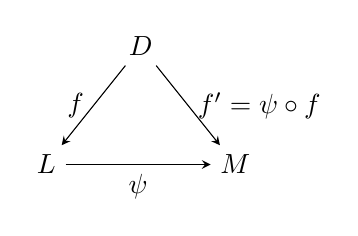
\begin{tikzpicture}[>=stealth,scale=1.0]
\node (D) at (0,0) {\(D\)};
\node (L) at (-1.2,-1.5) {\(L\)};
\node (M) at (1.2,-1.5) {\(M\)};
\draw[->] (D) -- node[left]{\(f\)} (L);
\draw[->] (D) -- node[right]{\(f'=\psi\circ f\)} (M);
\draw[->] (L) -- node[below]{\(\psi\)} (M);
\end{tikzpicture}\end{center}
图示。换句话说，与 \(\psi\) 复合诱导出映射
\[
\psi' : \operatorname{Hom}_R(D, L) \to \operatorname{Hom}_R(D, M), \qquad f \mapsto f' = \psi \circ f.
\]
回忆由命题 \ref{pro:10.2}，\(\operatorname{Hom}_R(D, L)\) 与 \(\operatorname{Hom}_R(D, M)\) 是阿贝尔群。

\begin{proposition}\label{pro:10.27}
设 \(D, L, M\) 是 \(R\)-模，\(\psi : L \to M\) 是 \(R\)-模同态。则映射
\[
\psi' : \operatorname{Hom}_R(D, L) \to \operatorname{Hom}_R(D, M), \qquad f \mapsto f' = \psi \circ f
\]
是阿贝尔群的同态。若 \(\psi\) 是单射，则 \(\psi'\) 也是单射，即若 \(0 \to L \xrightarrow{\psi} M\) 正合，则 \(0 \to \operatorname{Hom}_R(D, L) \xrightarrow{\psi'} \operatorname{Hom}_R(D, M)\) 也正合。
\end{proposition}

\begin{proof}
\(\psi'\) 是同态这一事实是直接的。若 \(\psi\) 是单射，则从 \(D\) 到 \(L\) 的两个不同同态 \(f\) 与 \(g\) 给出从 \(D\) 到 \(M\) 的两个不同同态 \(\psi \circ f\) 与 \(\psi \circ g\)，这就是说 \(\psi'\) 也是单射。
\end{proof}

从到子模 \(L\) 的同态得到到 \(M\) 的同态是直接的，而从到商 \(N\) 的同态出发的情形就不那么明显了。更精确地说，给定 \(R\)-模同态 \(f : D \to N\)，问题是是否存在 \(R\)-模同态 \(F : D \to M\) 把 \(f\) \textbf{延拓}或\textbf{提升}到 \(M\)，即使下图交换：
\begin{center}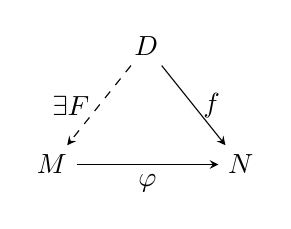
\begin{tikzpicture}[>=stealth,scale=1.0]
\node (D) at (0,0) {\(D\)};
\node (M) at (-1.2,-1.5) {\(M\)};
\node (N) at (1.2,-1.5) {\(N\)};
\draw[->] (D) -- node[right]{\(f\)} (N);
\draw[->] (M) -- node[below]{\(\varphi\)} (N);
\draw[->,dashed] (D) -- node[left]{\(\exists F\)} (M);
\end{tikzpicture}\end{center}
和前面一样，与同态 \(\varphi\) 复合诱导出阿贝尔群的同态
\[
\varphi' : \operatorname{Hom}_R(D, M) \to \operatorname{Hom}_R(D, N), \qquad F \mapsto F' = \varphi \circ F.
\]
用 \(\varphi'\) 来说，从 \(N\) 到 \(M\) 的同态 \(f\) 能提升为到 \(M\) 的同态当且仅当 \(f\) 在 \(\varphi'\) 的像中（即 \(f\) 是某个提升 \(F\) 的像）。

一般地可能无法把从 \(D\) 到 \(N\) 的同态 \(f\) 提升为从 \(D\) 到 \(M\) 的同态。例如考虑前面一组例子中的不分裂正合列 \(0 \to \mathbb{Z} \xrightarrow{\times 2} \mathbb{Z} \to \mathbb{Z}/2\mathbb{Z} \to 0\). 取 \(D = \mathbb{Z}/2\mathbb{Z}\)，\(f\) 为从 \(D\) 到 \(N\) 的恒等映射。从 \(D\) 到 \(M = \mathbb{Z}\) 的任何同态 \(F\) 都把 \(D\) 映到 0（因为 \(\mathbb{Z}\) 没有 2 阶元素），故 \(\pi \circ F\) 把 \(D\) 映到 \(N\) 中的 0，特别地 \(\pi \circ F \neq f\). 用映射 \(\varphi'\) 来说，这表明
\[
\text{若 } M \xrightarrow{\varphi} N \to 0 \text{ 正合，则 } \operatorname{Hom}_R(D, M) \xrightarrow{\varphi'} \operatorname{Hom}_R(D, N) \to 0 \text{ 不一定正合}。
\]

这些把到 \(L\) 与到 \(N\) 的同态与到 \(M\) 的同态联系起来的结果，可以整齐地概括为下面定理的一部分。

\begin{theorem}\label{thm:10.28}
设 \(D, L, M, N\) 是 \(R\)-模。若
\[
0 \longrightarrow L \xrightarrow{\ \psi\ } M \xrightarrow{\ \varphi\ } N \longrightarrow 0
\]
正合，则相应的序列
\begin{equation}
0 \longrightarrow \operatorname{Hom}_R(D, L) \xrightarrow{\ \psi'\ } \operatorname{Hom}_R(D, M) \xrightarrow{\ \varphi'\ } \operatorname{Hom}_R(D, N) \tag{10.10}
\end{equation}
正合。同态 \(f : D \to N\) 能提升为同态 \(F : D \to M\) 当且仅当 \(f \in \operatorname{Hom}_R(D, N)\) 在 \(\varphi'\) 的像中。一般地 \(\varphi' : \operatorname{Hom}_R(D, M) \to \operatorname{Hom}_R(D, N)\) 不必是满射；\(\varphi'\) 是满射当且仅当每个从 \(D\) 到 \(N\) 的同态都提升为从 \(D\) 到 \(M\) 的同态，此时序列（10.10）可以延拓为短正合列。

序列（10.10）对所有 \(R\)-模 \(D\) 都正合，当且仅当序列 \(0 \to L \xrightarrow{\psi} M \xrightarrow{\varphi} N\) 正合。
\end{theorem}

\begin{proof}
第一个论断中唯一尚未证明的是（10.10）在 \(\operatorname{Hom}_R(D, M)\) 处的正合性，即 \(\ker\varphi' = \mathrm{image}\,\psi'\). 假设 \(F : D \to M\) 是 \(\operatorname{Hom}_R(D, M)\) 中落在 \(\varphi'\) 的核中的元素，即作为从 \(D\) 到 \(N\) 的同态有 \(\varphi \circ F = 0\). 若 \(d \in D\) 是 \(D\) 的任意元素，这意味着 \(\varphi(F(d)) = 0\) 且 \(F(d) \in \ker\varphi\). 由定义扩张 \(M\) 的序列的正合性有 \(\ker\varphi = \mathrm{image}\,\psi\)，故存在某个元素 \(l \in L\) 使 \(F(d) = \psi(l)\). 由于 \(\psi\) 是单射，元素 \(l\) 唯一，故这给出有定义的映射 \(F' : D \to L\)，\(F'(d) = l\). 容易验证 \(F'\) 是同态，即 \(F' \in \operatorname{Hom}_R(D, L)\). 由于 \(\psi \circ F'(d) = \psi(l) = F(d)\)，我们有 \(F = \psi'(F')\)，这表明 \(F\) 在 \(\psi'\) 的像中，证明了 \(\ker\varphi' \subseteq \mathrm{image}\,\psi'\). 反之，若 \(F\) 在 \(\psi'\) 的像中，则对某个 \(F' \in \operatorname{Hom}_R(D, L)\) 有 \(F = \psi'(F')\)，于是对任意 \(d \in D\) 有 \(\varphi(F(d)) = \varphi(\psi(F'(d)))\). 由于 \(\ker\varphi = \mathrm{image}\,\psi\)，有 \(\varphi \circ \psi = 0\)，从而对任意 \(d \in D\) 有 \(\varphi(F(d)) = 0\)，即 \(\varphi'(F) = 0\). 于是 \(F\) 在 \(\varphi'\) 的核中，证明了反向包含：\(\mathrm{image}\,\psi' \supseteq \ker\varphi'\).

对于定理的最后一个论断，首先注意在证明（10.10）正合时并未用到 \(\varphi\) 的满射性，故该论断的“若”部分已经证明。反之，假设序列（10.10）对所有 \(R\)-模 \(D\) 都正合。一般地对任意左 \(R\)-模 \(X\) 有 \(\operatorname{Hom}_R(R, X) \cong X\)，同构由把同态映到它在元素 \(1_R \in R\) 处的取值给出（参见习题 10（b））。在（10.10）中取 \(D = R\)，容易得出序列 \(0 \to L \xrightarrow{\psi} M \xrightarrow{\varphi} N\) 的正合性。
\end{proof}

由定理 \ref{thm:10.28}，序列
\begin{equation}
0 \longrightarrow \operatorname{Hom}_R(D, L) \xrightarrow{\ \psi'\ } \operatorname{Hom}_R(D, M) \xrightarrow{\ \varphi'\ } \operatorname{Hom}_R(D, N) \longrightarrow 0 \tag{10.11}
\end{equation}
一般不是短正合列，因为同态 \(\varphi'\) 不必是满射。这个序列是否正合，恰好衡量了从 \(D\) 到 \(M\) 的同态在多大程度上由从 \(D\) 到 \(L\) 与从 \(D\) 到 \(N\) 的同态对唯一确定。更精确地说，这个序列正合当且仅当在从 \(D\) 到 \(M\) 的同态 \(F\) 与同态对 \((g, f)\)（\(g : D \to L\)，\(f : D \to N\)）之间存在由 \(F|_{\psi(L)} = \psi'(g)\) 与 \(f = \varphi'(F)\) 给出的双射 \(F \leftrightarrow (g, f)\).

序列（10.11）正合的一个情形是原来的序列 \(0 \to L \to M \to N \to 0\) 是分裂正合列，即 \(M = L \oplus N\) 的时候。此时序列（10.11）也是分裂正合列，如下一个命题的第一部分所示。

\begin{proposition}\label{pro:10.29}
设 \(D, L, N\) 是 \(R\)-模。则

（1）\(\operatorname{Hom}_R(D, L \oplus N) \cong \operatorname{Hom}_R(D, L) \oplus \operatorname{Hom}_R(D, N)\)，且

（2）\(\operatorname{Hom}_R(L \oplus N, D) \cong \operatorname{Hom}_R(L, D) \oplus \operatorname{Hom}_R(N, D)\).
\end{proposition}

\begin{proof}
设 \(\pi_1 : L \oplus N \to L\) 是从 \(L \oplus N\) 到 \(L\) 的自然投影，同样设 \(\pi_2\) 是到 \(N\) 的投影。若 \(f \in \operatorname{Hom}_R(D, L \oplus N)\)，则复合 \(\pi_1 \circ f\) 与 \(\pi_2 \circ f\) 分别给出 \(\operatorname{Hom}_R(D, L)\) 与 \(\operatorname{Hom}_R(D, N)\) 中的元素。这定义了一个从 \(\operatorname{Hom}_R(D, L \oplus N)\) 到 \(\operatorname{Hom}_R(D, L) \oplus \operatorname{Hom}_R(D, N)\) 的映射，容易看出它是同态。反之，给定 \(f_1 \in \operatorname{Hom}_R(D, L)\) 与 \(f_2 \in \operatorname{Hom}_R(D, N)\)，由 \(f(d) = (f_1(d), f_2(d))\) 定义映射 \(f \in \operatorname{Hom}_R(D, L \oplus N)\). 这定义了一个从 \(\operatorname{Hom}_R(D, L) \oplus \operatorname{Hom}_R(D, N)\) 到 \(\operatorname{Hom}_R(D, L \oplus N)\) 的映射，容易验证它是上面映射的逆同态，证明了（1）中的同构。（2）的证明类似，留作习题。
\end{proof}

命题 \ref{pro:10.29} 中的结果立即由归纳推广到任意有限个 \(R\)-模的直和。这些结果被说成是“\(\operatorname{Hom}\) 在两个变量上与有限直和交换”（与定理 \ref{thm:10.17} 中张量积的相应结果比较）。对无限直和情形更复杂。若把 \(L \oplus N\) 换成任意直和、并把右端的直和换成直积，则（1）仍然成立（习题 13 表明直积是必要的）。（2）若把两边的直和都换成直积也仍然成立。

这个命题表明，若
\[
0 \longrightarrow L \xrightarrow{\ \psi\ } M \xrightarrow{\ \varphi\ } N \longrightarrow 0
\]
是 \(R\)-模的分裂短正合列，则对每个 \(R\)-模 \(D\)，
\[
0 \longrightarrow \operatorname{Hom}_R(D, L) \xrightarrow{\ \psi'\ } \operatorname{Hom}_R(D, M) \xrightarrow{\ \varphi'\ } \operatorname{Hom}_R(D, N) \longrightarrow 0
\]
也是阿贝尔群的分裂短正合列。习题 14 表明其逆也成立：若 \(0 \to \operatorname{Hom}_R(D, L) \xrightarrow{\psi'} \operatorname{Hom}_R(D, M) \xrightarrow{\varphi'} \operatorname{Hom}_R(D, N) \to 0\) 对每个 \(R\)-模 \(D\) 都正合，则 \(0 \to L \xrightarrow{\psi} M \xrightarrow{\varphi} N \to 0\) 是分裂短正合列（这又蕴涵：若原来的 \(\operatorname{Hom}\) 序列对每个 \(D\) 都正合，则事实上它对每个 \(D\) 都是分裂正合的）。

命题 \ref{pro:10.29} 用模 \(L, M, N\) 确定了序列（10.11）正合的一个情形。下一个结果则采取稍稍不同的视角，转而刻画那些使定理 \ref{thm:10.28} 中的序列（10.10）总能延拓为短正合列的模 \(D\)：

\begin{proposition}\label{pro:10.30}
设 \(P\) 是 \(R\)-模。则下列命题等价：

（1）对任意 \(R\)-模 \(L, M, N\)，若
\[
0 \longrightarrow L \xrightarrow{\ \psi\ } M \xrightarrow{\ \varphi\ } N \longrightarrow 0
\]
是短正合列，则
\[
0 \longrightarrow \operatorname{Hom}_R(P, L) \xrightarrow{\ \psi'\ } \operatorname{Hom}_R(P, M) \xrightarrow{\ \varphi'\ } \operatorname{Hom}_R(P, N) \longrightarrow 0
\]
也是短正合列。

（2）对任意 \(R\)-模 \(M\) 和 \(N\)，若 \(M \xrightarrow{\varphi} N \to 0\) 正合，则从 \(P\) 到 \(N\) 的每个 \(R\)-模同态都提升为到 \(M\) 的 \(R\)-模同态，即给定 \(f \in \operatorname{Hom}_R(P, N)\)，存在提升 \(F \in \operatorname{Hom}_R(P, M)\) 使下图交换：
\begin{center}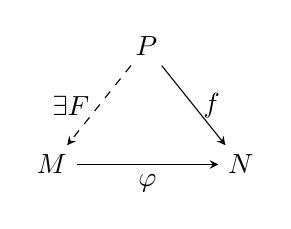
\begin{tikzpicture}[>=stealth,scale=1.0]
\node (P) at (0,0) {\(P\)};
\node (M) at (-1.2,-1.5) {\(M\)};
\node (N) at (1.2,-1.5) {\(N\)};
\draw[->] (P) -- node[right]{\(f\)} (N);
\draw[->] (M) -- node[below]{\(\varphi\)} (N);
\draw[->,dashed] (P) -- node[left]{\(\exists F\)} (M);
\end{tikzpicture}\end{center}

（3）若 \(P\) 是 \(R\)-模 \(M\) 的商模，则 \(P\) 同构于 \(M\) 的直和项，即每个短正合列 \(0 \to L \to M \to P \to 0\) 都分裂。

（4）\(P\) 是某个自由 \(R\)-模的直和项。
\end{proposition}

\begin{proof}
（1）与（2）的等价是定理 \ref{thm:10.28} 中结果的重新表述。现在假设（2）成立，并设 \(0 \to L \xrightarrow{\psi} M \xrightarrow{\varphi} P \to 0\) 正合。由（2），从 \(P\) 到 \(P\) 的恒等映射提升为同态 \(\mu\)，使下图交换：
\begin{center}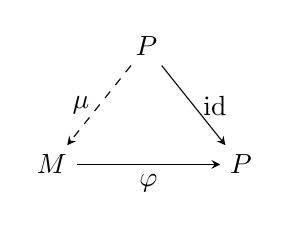
\begin{tikzpicture}[>=stealth,scale=1.0]
\node (P) at (0,0) {\(P\)};
\node (M) at (-1.2,-1.5) {\(M\)};
\node (P2) at (1.2,-1.5) {\(P\)};
\draw[->] (P) -- node[right]{\(\mathrm{id}\)} (P2);
\draw[->] (M) -- node[below]{\(\varphi\)} (P2);
\draw[->,dashed] (P) -- node[left]{\(\mu\)} (M);
\end{tikzpicture}\end{center}
则 \(\varphi \circ \mu = 1\)，故 \(\mu\) 是这个序列的分裂同态，这证明了（3）。每个模 \(P\) 都是自由模的商（例如取 \(P\) 的元素集合上的自由模），故总有正合列 \(0 \to \ker\varphi \to \mathcal{F} \xrightarrow{\varphi} P \to 0\)，其中 \(\mathcal{F}\) 是自由 \(R\)-模（参见推论 \ref{cor:10.23} 之后的例 4）。若（3）成立，则这个序列分裂，故 \(\mathcal{F}\) 同构于 \(\ker\varphi\) 与 \(P\) 的直和，这证明了（4）。

最后证明（4）蕴涵（2）。假设 \(P\) 是某个集合 \(S\) 上的自由 \(R\)-模的直和项，比如 \(\mathcal{F}(S) = P \oplus K\)，并给定如（2）中那样从 \(P\) 到 \(N\) 的同态 \(f\). 设 \(\pi\) 表示从 \(\mathcal{F}(S)\) 到 \(P\) 的自然投影，于是 \(f \circ \pi\) 是从 \(\mathcal{F}(S)\) 到 \(N\) 的同态。对任意 \(s \in S\) 定义 \(n_s = f \circ \pi(s) \in N\)，并取 \(m_s \in M\) 为满足 \(\varphi(m_s) = n_s\) 的任意元素（这样的元素存在，因为 \(\varphi\) 是满射）。由自由模的泛性质（第 10.3 节定理 \ref{thm:10.6}），存在唯一的 \(R\)-模同态 \(F'\) 从 \(\mathcal{F}(S)\) 到 \(M\) 且 \(F'(s) = m_s\). 图如下：
\begin{center}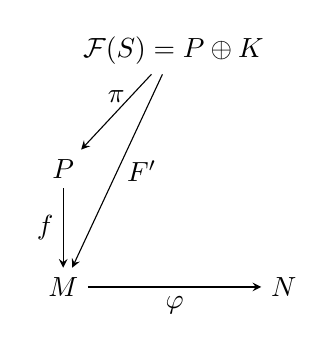
\begin{tikzpicture}[>=stealth,scale=1.0]
\node (F) at (0,0) {\(\mathcal{F}(S) = P \oplus K\)};
\node (P) at (-1.4,-1.5) {\(P\)};
\node (M) at (-1.4,-3) {\(M\)};
\node (N) at (1.4,-3) {\(N\)};
\draw[->] (F) -- node[above]{\(\pi\)} (P);
\draw[->] (F) -- node[right]{\(F'\)} (M);
\draw[->] (P) -- node[left]{\(f\)} (M);
\draw[->] (M) -- node[below]{\(\varphi\)} (N);
\end{tikzpicture}\end{center}
由同态 \(F'\) 的定义有 \(\varphi \circ F'(s) = \varphi(m_s) = n_s = f \circ \pi(s)\)，由此在 \(\mathcal{F}(S)\) 上 \(\varphi \circ F' = f \circ \pi\)，即上图交换。现在由 \(F(d) = F'((d, 0))\) 定义映射 \(F : P \to M\). 由于 \(F\) 是含入 \(P \to \mathcal{F}(S)\) 与同态 \(F'\) 的复合，可知 \(F\) 是 \(R\)-模同态。于是
\[
\varphi \circ F(d) = \varphi \circ F'((d, 0)) = f \circ \pi((d, 0)) = f(d),
\]
即 \(\varphi \circ F = f\)，故图
\begin{center}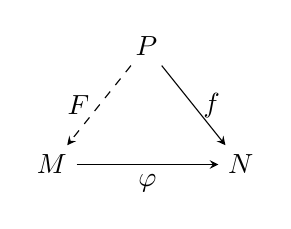
\begin{tikzpicture}[>=stealth,scale=1.0]
\node (P) at (0,0) {\(P\)};
\node (M) at (-1.2,-1.5) {\(M\)};
\node (N) at (1.2,-1.5) {\(N\)};
\draw[->] (P) -- node[right]{\(f\)} (N);
\draw[->] (M) -- node[below]{\(\varphi\)} (N);
\draw[->,dashed] (P) -- node[left]{\(F\)} (M);
\end{tikzpicture}\end{center}
交换，这证明了（4）蕴涵（2）并完成证明。
\end{proof}

\begin{definition}
满足命题 \ref{pro:10.30} 中任意一个等价条件的 \(R\)-模 \(P\) 称为\textbf{投射模}。
\end{definition}

命题 \ref{pro:10.30} 中的第三个命题可以重新表述为：任何满射到 \(P\) 的模 \(M\) 都以 \(P\)（的同构拷贝）作为直和项，这解释了“投射”这一术语。

下面的结果由命题 \ref{pro:10.30}（及其证明）立即得到：

\begin{corollary}\label{cor:10.31}
自由模是投射模。有限生成的模是投射模当且仅当它是有限生成自由模的直和项。每个模都是某个投射模的商模。
\end{corollary}

若 \(D\) 固定，则对任意 \(R\)-模 \(X\) 我们都有相应的阿贝尔群 \(\operatorname{Hom}_R(D, X)\). 进一步，\(R\)-模同态 \(\alpha : X \to Y\) 诱导出阿贝尔群同态 \(\alpha' : \operatorname{Hom}_R(D, X) \to \operatorname{Hom}_R(D, Y)\)，由 \(\alpha'(f) = \alpha \circ f\) 定义。换句话说，映射 \(\operatorname{Hom}_R(D, \_)\) 是从 \(R\)-模范畴到阿贝尔群范畴的\textbf{共变函子}（参见附录 II）。定理 \ref{thm:10.28} 表明，把这个函子作用到正合列
\[
0 \longrightarrow L \xrightarrow{\ \psi\ } M \xrightarrow{\ \varphi\ } N \longrightarrow 0
\]
的各项上，产生正合列
\[
0 \longrightarrow \operatorname{Hom}_R(D, L) \xrightarrow{\ \psi'\ } \operatorname{Hom}_R(D, M) \xrightarrow{\ \varphi'\ } \operatorname{Hom}_R(D, N).
\]
这被说成 \(\operatorname{Hom}_R(D, \_)\) 是\textbf{左正合函子}。由命题 \ref{pro:10.30}，函子 \(\operatorname{Hom}_R(D, \_)\) 正合（即总把短正合列变为短正合列）当且仅当 \(D\) 是投射模。我们把它总结为

\begin{corollary}\label{cor:10.32}
若 \(D\) 是 \(R\)-模，则从 \(R\)-模范畴到阿贝尔群范畴的函子 \(\operatorname{Hom}_R(D, \_)\) 是左正合的。它正合当且仅当 \(D\) 是投射 \(R\)-模。
\end{corollary}

注意若 \(\operatorname{Hom}_R(D, \_)\) 把短正合列变为短正合列，则它把任意长度的正合列变为正合列，因为任何正合列都可以分解为一系列短正合列。

如我们所看到的，函子 \(\operatorname{Hom}_R(D, \_)\) 一般在右边不正合。衡量诸如 \(\operatorname{Hom}_R(D, \_)\) 这样的函子不正合的程度，引出了第 17 章中考虑的“同调代数”的概念。

\begin{example}
（1）我们将在第 11.1 节看到，若 \(R = F\) 是域，则每个 \(F\)-模都是投射模（虽然我们只对有限生成模范证明这一点）。

（2）由推论 \ref{cor:10.31}，\(\mathbb{Z}\) 是投射 \(\mathbb{Z}\)-模。这也可以直接看出：假设 \(f\) 是从 \(\mathbb{Z}\) 到 \(N\) 的映射且 \(M \xrightarrow{\varphi} N \to 0\) 正合。同态 \(f\) 由值 \(n = f(1)\) 唯一确定。则 \(f\) 可以提升为同态 \(F : \mathbb{Z} \to M\)：先定义 \(F(1) = m\)，其中 \(m\) 是被 \(\varphi\) 映到 \(n\) 的 \(M\) 中任意元素，然后由加性把 \(F\) 延拓到整个 \(\mathbb{Z}\).

由命题 \ref{pro:10.30} 的第一个论断，由于 \(\mathbb{Z}\) 是投射模，若
\[
0 \longrightarrow L \xrightarrow{\ \psi\ } M \xrightarrow{\ \varphi\ } N \longrightarrow 0
\]
是 \(\mathbb{Z}\)-模的正合列，则
\[
0 \longrightarrow \operatorname{Hom}_{\mathbb{Z}}(\mathbb{Z}, L) \xrightarrow{\ \psi'\ } \operatorname{Hom}_{\mathbb{Z}}(\mathbb{Z}, M) \xrightarrow{\ \varphi'\ } \operatorname{Hom}_{\mathbb{Z}}(\mathbb{Z}, N) \longrightarrow 0
\]
也是正合列。这也可以直接用阿贝尔群的同构 \(\operatorname{Hom}_{\mathbb{Z}}(\mathbb{Z}, M) \cong M\) 看出，它表明上面两个正合列本质上是同一个。

（3）自由的 \(\mathbb{Z}\)-模没有非零有限阶元素，故没有非零有限阿贝尔群能同构于自由模的子模。由推论 \ref{cor:10.31} 可知没有非零有限阿贝尔群是投射 \(\mathbb{Z}\)-模。

（4）作为上一例的特殊情形，我们看到对 \(n \geq 2\)，\(\mathbb{Z}\)-模 \(\mathbb{Z}/n\mathbb{Z}\) 不是投射模。由定理 \ref{thm:10.28} 必能找到这样的短正合列，它对函子 \(\operatorname{Hom}_{\mathbb{Z}}(\mathbb{Z}/n\mathbb{Z}, \_)\) 作用后在右边不再正合。一个这样的序列就是推论 \ref{cor:10.23} 之后例子 2 中的正合列（对 \(n \geq 2\)）。首先注意 \(\operatorname{Hom}_{\mathbb{Z}}(\mathbb{Z}/n\mathbb{Z}, \mathbb{Z}) = 0\)，因为不存在从 \(\mathbb{Z}/n\mathbb{Z}\) 到 \(\mathbb{Z}\) 的非零 \(\mathbb{Z}\)-模同态。也容易看出 \(\operatorname{Hom}_{\mathbb{Z}}(\mathbb{Z}/n\mathbb{Z}, \mathbb{Z}/n\mathbb{Z}) \cong \mathbb{Z}/n\mathbb{Z}\)，如下：每个同态 \(f\) 由 \(f(1) = a \in \mathbb{Z}/n\mathbb{Z}\) 唯一确定，而给定任意 \(a \in \mathbb{Z}/n\mathbb{Z}\) 都有唯一同态 \(f_a\) 满足 \(f_a(1) = a\)；容易验证 \(f_a \mapsto a\) 是从 \(\operatorname{Hom}_{\mathbb{Z}}(\mathbb{Z}/n\mathbb{Z}, \mathbb{Z}/n\mathbb{Z})\) 到 \(\mathbb{Z}/n\mathbb{Z}\) 的同构。

于是把 \(\operatorname{Hom}_{\mathbb{Z}}(\mathbb{Z}/n\mathbb{Z}, \_)\) 作用到上面的短正合列上，得到序列
\[
0 \longrightarrow 0 \xrightarrow{\ 0\ } 0 \xrightarrow{\ \times n\ } \mathbb{Z}/n\mathbb{Z} \xrightarrow{\ \ } 0,
\]
它在唯一的非零项处不正合。

（5）由于 \(\mathbb{Q}/\mathbb{Z}\) 是挠 \(\mathbb{Z}\)-模，它不是自由 \(\mathbb{Z}\)-模的子模，故不是投射模。还要注意正合列 \(0 \to \mathbb{Z} \to \mathbb{Q} \to \mathbb{Q}/\mathbb{Z} \to 0\) 不分裂，因为 \(\mathbb{Q}\) 不含同构于 \(\mathbb{Q}/\mathbb{Z}\) 的子模。

（6）\(\mathbb{Z}\)-模 \(\mathbb{Q}\) 不是投射模（参见习题）。

（7）我们将在第 12 章看到，有限生成 \(\mathbb{Z}\)-模是投射模当且仅当它是自由模。

（8）设 \(R\) 是按逐分量加法与乘法构成的交换环 \(\mathbb{Z}/2\mathbb{Z} \times \mathbb{Z}/2\mathbb{Z}\). 若 \(P_1\) 与 \(P_2\) 分别是 \((1, 0)\) 与 \((0, 1)\) 生成的主理想，则 \(R = P_1 \oplus P_2\)，故由命题 \ref{pro:10.30}，\(P_1\) 与 \(P_2\) 都是投射 \(R\)-模。\(P_1\) 与 \(P_2\) 都不是自由模，因为任何自由模的阶都是 4 的倍数。

（9）两个投射模的直和仍是投射模（参见习题 3）。

（10）我们将在第 VI 部分看到，若 \(F\) 是任意域、\(n \in \mathbb{Z}^+\)，则元素取自 \(F\) 的全体 \(n \times n\) 矩阵构成的环 \(R = M_n(F)\) 具有“每个 \(R\)-模都是投射模”这一性质。我们还将看到，若 \(G\) 是阶为 \(n\) 的有限群且 \(n \neq 0\) 于域 \(F\) 中，则群环 \(FG\) 也具有“每个模都是投射模”这一性质。
\end{example}

\noindent\textbf{内射模与 \(\operatorname{Hom}_R(\_, D)\)}

若 \(0 \to L \xrightarrow{\psi} M \xrightarrow{\varphi} N \to 0\) 是 \(R\)-模的短正合列，则除了考虑从 \(R\)-模 \(D\) 到 \(L\) 或 \(N\) 的映射以及它们在多大程度上决定从 \(D\) 到 \(M\) 的映射之外，我们还可以考虑从 \(L\) 或 \(N\) 到 \(D\) 的映射这一“对偶”问题。此时从 \(N\) 到 \(D\) 的映射的情形很容易处理：从 \(N\) 到 \(D\) 的 \(R\)-模映射与 \(\varphi\) 复合立即给出从 \(M\) 到 \(D\) 的映射。容易验证这定义了阿贝尔群的单同态
\[
\varphi' : \operatorname{Hom}_R(N, D) \to \operatorname{Hom}_R(M, D), \qquad f \mapsto f' = f \circ \varphi,
\]
或换一种说法，
\[
\text{若 } M \xrightarrow{\varphi} N \to 0 \text{ 正合，则 } 0 \to \operatorname{Hom}_R(N, D) \xrightarrow{\varphi'} \operatorname{Hom}_R(M, D) \text{ 正合}。
\]
（注意同态群上相应的映射方向与原来的映射相反。）

另一方面，给定从 \(L\) 到 \(D\) 的 \(R\)-模同态 \(f\)，可能无法把 \(f\) 延拓为从 \(M\) 到 \(D\) 的映射，即给定 \(f\) 可能找不到使下图交换的映射 \(F\)：
\begin{center}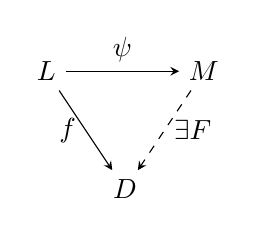
\begin{tikzpicture}[>=stealth,scale=1.0]
\node (L) at (0,0) {\(L\)};
\node (M) at (2,0) {\(M\)};
\node (D) at (1,-1.5) {\(D\)};
\draw[->] (L) -- node[above]{\(\psi\)} (M);
\draw[->] (L) -- node[left]{\(f\)} (D);
\draw[->,dashed] (M) -- node[right]{\(\exists F\)} (D);
\end{tikzpicture}\end{center}
例如考虑 \(\mathbb{Z}\)-模的正合列 \(0 \to \mathbb{Z} \xrightarrow{\times 2} \mathbb{Z} \to \mathbb{Z}/2\mathbb{Z} \to 0\)，其中 \(\psi\) 是乘以 2 而 \(\varphi\) 是自然投影。取 \(D = \mathbb{Z}/2\mathbb{Z}\)，并令 \(f : \mathbb{Z} \to \mathbb{Z}/2\mathbb{Z}\) 为序列中第一个 \(\mathbb{Z}\) 上的模 2 约化。从序列中第二个 \(\mathbb{Z}\) 到 \(\mathbb{Z}/2\mathbb{Z}\) 只有一个非零同态 \(F\)（即模 2 约化），但这个 \(F\) 不提升映射 \(f\)，因为 \(F \circ \psi(\mathbb{Z}) = F(2\mathbb{Z}) = 0\)，故 \(F \circ \psi \neq f\).

与 \(\psi\) 复合诱导出阿贝尔群同态 \(\psi'\) 从 \(\operatorname{Hom}_R(M, D)\) 到 \(\operatorname{Hom}_R(L, D)\)，而用映射 \(\psi'\) 来说，同态 \(f \in \operatorname{Hom}_R(L, D)\) 能提升为从 \(M\) 到 \(D\) 的同态当且仅当 \(f\) 在 \(\psi'\) 的像中。上面的例子表明
\[
\text{若 } 0 \to L \xrightarrow{\psi} M \text{ 正合，则 } \operatorname{Hom}_R(M, D) \xrightarrow{\psi'} \operatorname{Hom}_R(L, D) \to 0 \text{ 不一定正合}。
\]

我们可以把这些结果概括为定理 \ref{thm:10.28} 的下面对偶形式：

\begin{theorem}\label{thm:10.33}
设 \(D, L, M, N\) 是 \(R\)-模。若
\[
0 \longrightarrow L \xrightarrow{\ \psi\ } M \xrightarrow{\ \varphi\ } N \longrightarrow 0
\]
正合，则相应的序列
\begin{equation}
0 \longrightarrow \operatorname{Hom}_R(N, D) \xrightarrow{\ \varphi'\ } \operatorname{Hom}_R(M, D) \xrightarrow{\ \psi'\ } \operatorname{Hom}_R(L, D) \tag{10.12}
\end{equation}
正合。同态 \(f : L \to D\) 能提升为同态 \(F : M \to D\) 当且仅当 \(f \in \operatorname{Hom}_R(L, D)\) 在 \(\psi'\) 的像中。一般地 \(\psi' : \operatorname{Hom}_R(M, D) \to \operatorname{Hom}_R(L, D)\) 不必是满射；\(\psi'\) 是满射当且仅当每个从 \(L\) 到 \(D\) 的同态都提升为从 \(M\) 到 \(D\) 的同态，此时序列（10.12）可以延拓为短正合列。

序列（10.12）对所有 \(R\)-模 \(D\) 都正合，当且仅当序列 \(L \xrightarrow{\psi} M \xrightarrow{\varphi} N \to 0\) 正合。
\end{theorem}

\begin{proof}
第一个论断中剩下的唯一待证项是（10.12）在 \(\operatorname{Hom}_R(M, D)\) 处的正合性。这个断言的证明与定理 \ref{thm:10.28} 中相应结果的证明非常类似，留作习题。还要注意这里不需要 \(\psi\) 是单射，这证明了定理最后一个论断的“若”部分。

现在假设序列（10.12）对所有 \(R\)-模 \(D\) 都正合。我们首先证明 \(\varphi : M \to N\) 是满射。取 \(D = N/\varphi(M)\). 若 \(\pi_1 : N \to N/\varphi(M)\) 是自然投影同态，则按 \(\pi_1\) 的定义有 \(\pi_1 \circ \varphi(M) = 0\). 由于 \(\pi_1 \circ \varphi = \varphi'(\pi_1)\)，这意味着元素 \(\pi_1 \in \operatorname{Hom}_R(N, N/\varphi(M))\) 被 \(\psi'\) 映到 0. 由于假设对所有的模 \(D\) 都有 \(\psi'\) 是单射，这意味着 \(\pi_1\) 是零映射，即 \(N/\varphi(M) = 0\)，故 \(\varphi\) 是满射。接下来我们证明 \(\varphi \circ \psi = 0\)，这将蕴涵 \(\mathrm{image}\,\psi \subseteq \ker\varphi\). 为此取 \(D = N\) 并注意 \(N\) 上的恒等映射 \(\mathrm{id}_N\) 含于 \(\operatorname{Hom}_R(N, N)\)，故 \(\varphi'(\mathrm{id}_N) \in \operatorname{Hom}_R(M, N)\). 于是（10.12）对 \(D = N\) 的正合性蕴涵 \(\varphi'(\mathrm{id}_N) \in \ker\psi'\)，故 \(\psi'(\varphi'(\mathrm{id}_N)) = 0\). 于是 \(\mathrm{id}_N \circ \varphi \circ \psi = 0\)，即 \(\varphi \circ \psi = 0\)，如所断言。最后我们证明 \(\ker\varphi \subseteq \mathrm{image}\,\psi\). 取 \(D = M/\psi(L)\)，并设 \(\pi_2 : M \to M/\psi(L)\) 是自然投影。则 \(\psi'(\pi_2) = 0\)，因为按 \(\pi_2\) 的定义有 \(\pi_2(\psi(L)) = 0\). （10.12）对这个 \(D\) 的正合性于是蕴涵 \(\pi_2\) 在 \(\varphi'\) 的像中，比如 \(\pi_2 = \varphi'(f)\) 对某个同态 \(f \in \operatorname{Hom}_R(N, M/\psi(L))\) 成立，即 \(\pi_2 = f \circ \varphi\). 若 \(m \in \ker\varphi\)，则 \(\pi_2(m) = f(\varphi(m)) = 0\)，而由于 \(\pi_2\) 正是从 \(M\) 到商 \(M/\psi(L)\) 的投影，这意味着 \(m \in \psi(L)\). 于是 \(\ker\varphi \subseteq \mathrm{image}\,\psi\)，完成证明。
\end{proof}

由定理 \ref{thm:10.33}，序列
\[
0 \longrightarrow \operatorname{Hom}_R(N, D) \xrightarrow{\ \varphi'\ } \operatorname{Hom}_R(M, D) \xrightarrow{\ \psi'\ } \operatorname{Hom}_R(L, D) \longrightarrow 0
\]
一般不是短正合列，因为 \(\psi'\) 不必是满射，而这个序列是否正合恰好衡量了从 \(M\) 到 \(D\) 的同态在多大程度上由从 \(L\) 与 \(N\) 到 \(D\) 的同态对唯一确定。

命题 \ref{pro:10.29} 中的第二个论断表明，当原来的正合列 \(0 \to L \xrightarrow{\psi} M \xrightarrow{\varphi} N \to 0\) 是分裂正合列时这个序列正合。事实上此时对每个 \(R\)-模 \(D\)，序列 \(0 \to \operatorname{Hom}_R(N, D) \xrightarrow{\varphi'} \operatorname{Hom}_R(M, D) \xrightarrow{\psi'} \operatorname{Hom}_R(L, D) \to 0\) 也是阿贝尔群的分裂正合列。习题 14 表明其逆也成立：若 \(0 \to \operatorname{Hom}_R(N, D) \xrightarrow{\varphi'} \operatorname{Hom}_R(M, D) \xrightarrow{\psi'} \operatorname{Hom}_R(L, D) \to 0\) 对每个 \(R\)-模 \(D\) 都正合，则 \(0 \to L \xrightarrow{\psi} M \xrightarrow{\varphi} N \to 0\) 是分裂短正合列（这又蕴涵：若这个 \(\operatorname{Hom}\) 序列对每个 \(D\) 都正合，则事实上它对每个 \(D\) 都是分裂正合的）。

命题 \ref{pro:10.30} 的前三部分也有对偶版本，它刻画了使定理 \ref{thm:10.33} 中的序列（10.12）总能延拓为短正合列的 \(R\)-模 \(D\)：

\begin{proposition}\label{pro:10.34}
设 \(Q\) 是 \(R\)-模。则下列命题等价：

（1）对任意 \(R\)-模 \(L, M, N\)，若
\[
0 \longrightarrow L \xrightarrow{\ \psi\ } M \xrightarrow{\ \varphi\ } N \longrightarrow 0
\]
是短正合列，则
\[
0 \longrightarrow \operatorname{Hom}_R(N, Q) \xrightarrow{\ \varphi'\ } \operatorname{Hom}_R(M, Q) \xrightarrow{\ \psi'\ } \operatorname{Hom}_R(L, Q) \longrightarrow 0
\]
也是短正合列。

（2）对任意 \(R\)-模 \(L\) 与 \(M\)，若 \(0 \to L \xrightarrow{\psi} M\) 正合，则从 \(L\) 到 \(Q\) 的每个 \(R\)-模同态都提升为从 \(M\) 到 \(Q\) 的 \(R\)-模同态，即给定 \(f \in \operatorname{Hom}_R(L, Q)\)，存在提升 \(F \in \operatorname{Hom}_R(M, Q)\) 使下图交换：
\begin{center}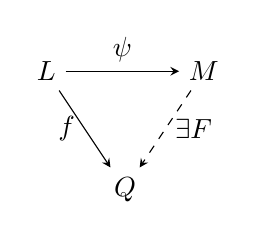
\begin{tikzpicture}[>=stealth,scale=1.0]
\node (M) at (2,0) {\(M\)};
\node (L) at (0,0) {\(L\)};
\node (Q) at (1,-1.5) {\(Q\)};
\draw[->] (L) -- node[above]{\(\psi\)} (M);
\draw[->] (L) -- node[left]{\(f\)} (Q);
\draw[->,dashed] (M) -- node[right]{\(\exists F\)} (Q);
\end{tikzpicture}\end{center}

（3）若 \(Q\) 是 \(R\)-模 \(M\) 的子模，则 \(Q\) 是 \(M\) 的直和项，即每个短正合列 \(0 \to Q \to M \to N \to 0\) 都分裂。
\end{proposition}

\begin{proof}
（1）与（2）的等价是定理 \ref{thm:10.33} 的一部分。现在假设（2）成立，并设 \(0 \to Q \xrightarrow{\psi} M \xrightarrow{\varphi} N \to 0\) 正合。取 \(L = Q\)，\(f\) 为从 \(Q\) 到自身的恒等映射，由（2）可知存在同态 \(F : M \to Q\) 使 \(F \circ \psi = 1\)，故 \(F\) 是这个序列的分裂同态，这证明了（3）。（3）蕴涵（2）的证明在习题中给出。
\end{proof}

\begin{definition}
满足命题 \ref{pro:10.34} 中任意一个等价条件的 \(R\)-模 \(Q\) 称为\textbf{内射模}。
\end{definition}

命题 \ref{pro:10.34} 中的第三个命题可以重新表述为：任何 \(Q\) 单射地映入其中的模 \(M\) 都以 \(Q\)（的同构拷贝）作为直和项，这解释了“内射”这一术语。

若 \(D\) 固定，则对任意 \(R\)-模 \(X\) 我们都有相应的阿贝尔群 \(\operatorname{Hom}_R(X, D)\). 进一步，\(R\)-模同态 \(\alpha : X \to Y\) 诱导出阿贝尔群同态 \(\alpha' : \operatorname{Hom}_R(Y, D) \to \operatorname{Hom}_R(X, D)\)，由 \(\alpha'(f) = f \circ \alpha\) 定义，它“反转”了箭头的方向。换句话说，映射 \(\operatorname{Hom}_R(\_, D)\) 是从 \(R\)-模范畴到阿贝尔群范畴的\textbf{反变函子}（参见附录 II）。定理 \ref{thm:10.33} 表明，把这个函子作用到正合列
\[
0 \longrightarrow L \xrightarrow{\ \psi\ } M \xrightarrow{\ \varphi\ } N \longrightarrow 0
\]
的各项上，产生正合列
\[
0 \longrightarrow \operatorname{Hom}_R(N, D) \xrightarrow{\ \varphi'\ } \operatorname{Hom}_R(M, D) \xrightarrow{\ \psi'\ } \operatorname{Hom}_R(L, D).
\]
这被说成 \(\operatorname{Hom}_R(\_, D)\) 是\textbf{左正合（反变）函子}。注意函子 \(\operatorname{Hom}_R(\_, D)\) 与前面考虑的函子 \(\operatorname{Hom}_R(D, \_)\) 都是左正合的；前者反转原短正合列中映射的方向，后者保持映射的方向。

由命题 \ref{pro:10.34}，函子 \(\operatorname{Hom}_R(\_, D)\) 正合（即总把短正合列变为短正合列，从而把任意长度的正合列变为正合列）当且仅当 \(D\) 是内射模。我们把它总结为下面这个命题，它与推论 \ref{cor:10.32} 的共变结果对偶。

\begin{corollary}\label{cor:10.35}
若 \(D\) 是 \(R\)-模，则从 \(R\)-模范畴到阿贝尔群范畴的函子 \(\operatorname{Hom}_R(\_, D)\) 是左正合的。它正合当且仅当 \(D\) 是内射 \(R\)-模。
\end{corollary}

我们已经看到 \(R\)-模是投射模当且仅当它是自由 \(R\)-模的直和项。给出内射 \(R\)-模如此简单的刻画就不那么容易了。下一个结果给出 \(Q\) 是内射 \(R\)-模的一个判别法（这个结果属于 Baer，他在 1940 年前后引入了内射模的概念），利用它可以对 \(R = \mathbb{Z}\)（或更一般地对 \(R\) 是主理想整环）的情形给出内射模的刻画。回忆称一个 \(\mathbb{Z}\)-模 \(A\)（即加法书写的阿贝尔群）是\textbf{可除的}，若对所有非零整数 \(n\) 有 \(A = nA\). 例如 \(\mathbb{Q}\) 与 \(\mathbb{Q}/\mathbb{Z}\) 都是可除的（参见第 2.4 节习题 18 和 19 以及第 3.1 节习题 15）。

\begin{proposition}\label{pro:10.36}
设 \(Q\) 是 \(R\)-模。

（1）（\textbf{Baer 判别法}）模 \(Q\) 是内射模当且仅当对 \(R\) 的每个左理想 \(I\)，任何 \(R\)-模同态 \(g : I \to Q\) 都可以延拓为 \(R\)-模同态 \(G : R \to Q\).

（2）若 \(R\) 是主理想整环，则 \(Q\) 是内射模当且仅当对所有非零 \(r \in R\) 有 \(rQ = Q\). 特别地，一个 \(\mathbb{Z}\)-模是内射模当且仅当它是可除的。当 \(R\) 是主理想整环时，内射 \(R\)-模的商模仍是内射模。
\end{proposition}

\begin{proof}
若 \(Q\) 是内射模且 \(g : I \to Q\) 是从 \(R\) 的非零理想 \(I\) 到 \(Q\) 的 \(R\)-模同态，则由把命题 \ref{pro:10.34}（2）应用于正合列 \(0 \to I \to R\)，可以把 \(g\) 延拓为从 \(R\) 到 \(Q\) 的 \(R\)-模同态，这证明了（1）的“仅当”部分。反之，假设每个同态 \(g : I \to Q\) 都可以提升为同态 \(G : R \to Q\). 为证明 \(Q\) 是内射模，我们必须证明若 \(0 \to L \xrightarrow{\psi} M\) 正合且 \(f : L \to Q\) 是 \(R\)-模同态，则存在延拓 \(f\) 的提升 \(F : M \to Q\). 若 \(S\) 是把 \(f\) 提升到包含 \(L\) 的 \(M\) 的子模 \(L'\) 的（\(f', L'\)）的集合，其中 \(f' : L' \to Q\)，定义序 \((f', L') \leq (f'', L'')\) 当且仅当 \(L' \subseteq L''\) 且 \(f''\) 在 \(L'\) 上等于 \(f'\)，则 \(S\) 被这个序半序化。由于 \(S \neq \varnothing\)，由佐恩引理 \(S\) 有极大元 \((F, M')\). 映射 \(F : M' \to Q\) 是 \(f\) 的提升，只需证明 \(M' = M\). 假设存在元素 \(m \in M\) 不属于 \(M'\)，并令 \(I = \{r \in R \mid rm \in M'\}\). 容易验证 \(I\) 是 \(R\) 的左理想，而由 \(g(x) = F(xm)\) 定义的映射 \(g : I \to Q\) 是从 \(I\) 到 \(Q\) 的 \(R\)-模同态。由假设存在 \(g\) 的提升 \(G : R \to Q\). 考虑 \(M\) 的子模 \(M'+Rm\)，并定义映射 \(F' : M'+Rm \to Q\) 为 \(F'(m'+rm) = F(m')+G(r)\). 若 \(m_1+r_1m = m_2+r_2m\)，则 \((r_1-r_2)m = m_2-m_1\) 表明 \(r_1-r_2 \in I\)，故
\[
G(r_1-r_2) = g(r_1-r_2) = F((r_1-r_2)m) = F(m_2-m_1),
\]
于是 \(F(m_1)+G(r_1) = F(m_2)+G(r_2)\). 因此 \(F'\) 有定义，且立即看出 \(F'\) 是把 \(f\) 延拓到 \(M'+Rm\) 的 \(R\)-模同态。这与 \(M'\) 的极大性矛盾，故 \(M' = M\)，这完成了（1）的证明。

为证明（2），假设 \(R\) 是主理想整环。\(R\) 的任何非零理想都有形式 \(I = (r)\)（\(r\) 是 \(R\) 的某个非零元素）。\(R\)-模同态 \(f : I \to Q\) 完全由像 \(f(r) = q \in Q\) 确定。这个同态能延拓为同态 \(F : R \to Q\) 当且仅当存在元素 \(q' \in Q\) 使 \(F(1) = q'\) 且满足 \(q = f(r) = F(r) = rq'\). 由此 \(Q\) 满足 Baer 判别法当且仅当 \(rQ = Q\)，这证明了（2）中前两个断言。（2）中最后一个断言由以下事实推出：若对 \(R\) 中所有 \(r \neq 0\) 有 \(rQ = Q\)，则 \(Q\) 的商模具有同样的性质。
\end{proof}

\begin{example}
（1）由于 \(\mathbb{Z}\) 不可除，\(\mathbb{Z}\) 不是内射 \(\mathbb{Z}\)-模。这也可以从对应于乘以 2 的正合列 \(0 \to \mathbb{Z} \xrightarrow{\times 2} \mathbb{Z} \to \mathbb{Z}/2\mathbb{Z} \to 0\) 不分裂这一事实推出。

（2）有理数 \(\mathbb{Q}\) 是内射 \(\mathbb{Z}\)-模。

（3）内射 \(\mathbb{Z}\)-模 \(\mathbb{Q}\) 的商 \(\mathbb{Q}/\mathbb{Z}\) 是内射 \(\mathbb{Z}\)-模。

（4）显然可除 \(\mathbb{Z}\)-模的直和仍可除，故内射 \(\mathbb{Z}\)-模的直和仍内射。例如 \(\mathbb{Q} \oplus \mathbb{Q}/\mathbb{Z}\) 是内射 \(\mathbb{Z}\)-模。（另见习题 4。）

（5）我们将在第 12 章看到，没有非零的有限生成 \(\mathbb{Z}\)-模是内射模。

（6）假设环 \(R\) 是整环。若对所有非零 \(r \in R\) 有 \(A = rA\)，则称 \(R\)-模 \(A\) 是\textbf{可除 \(R\)-模}。命题 \ref{pro:10.36} 的证明表明，此时内射 \(R\)-模是可除的。

（7）我们将在第 11.1 节看到，若 \(R = F\) 是域，则每个 \(F\)-模都是内射模。

（8）我们将在第 VI 部分看到，若 \(F\) 是任意域、\(n \in \mathbb{Z}^+\)，则元素取自 \(F\) 的全体 \(n \times n\) 矩阵构成的环 \(R = M_n(F)\) 具有“每个 \(R\)-模都是内射模（也是投射模）”这一性质。我们还将看到，若 \(G\) 是阶为 \(n\) 的有限群且 \(n \neq 0\) 于域 \(F\) 中，则群环 \(FG\) 也具有“每个模都是内射模（也是投射模）”这一性质。
\end{example}

\begin{corollary}\label{cor:10.37}
每个 \(\mathbb{Z}\)-模都是某个内射 \(\mathbb{Z}\)-模的子模。
\end{corollary}

\begin{proof}
设 \(M\) 是 \(\mathbb{Z}\)-模，\(A\) 是 \(M\) 的任意一组 \(\mathbb{Z}\)-模生成元。设 \(\mathcal{F} = F(A)\) 是集合 \(A\) 上的自由 \(\mathbb{Z}\)-模。则由定理 \ref{thm:10.6} 存在从 \(\mathcal{F}\) 到 \(M\) 的满 \(\mathbb{Z}\)-模同态，若用 \(K\) 表示这个同态的核，则 \(K\) 是 \(\mathcal{F}\) 的 \(\mathbb{Z}\)-子模，且可以把 \(M\) 与 \(\mathcal{F}/K\) 等同。设 \(Q\) 是集合 \(A\) 上的自由 \(\mathbb{Q}\)-模。则 \(Q\) 是若干份 \(\mathbb{Q}\) 的直和，因而是可除的，从而（由命题 \ref{pro:10.36}）是内射的 \(\mathbb{Z}\)-模，且包含 \(\mathcal{F}\). 于是 \(K\) 也是 \(Q\) 的 \(\mathbb{Z}\)-子模，故由命题 \ref{pro:10.36} 再次可知商 \(Q/K\) 是内射的。由于 \(M = \mathcal{F}/K \subseteq Q/K\)，可知 \(M\) 含于一个内射 \(\mathbb{Z}\)-模中。
\end{proof}

推论 \ref{cor:10.37} 可以用来证明下面的、对任意 \(R\)-模都成立的更一般的版本。这个定理是定理 \ref{thm:10.6} 与推论 \ref{cor:10.31} 中“每个 \(R\)-模都是投射 \(R\)-模的商模”这一结果的内射类似物。

\begin{theorem}\label{thm:10.38}
设 \(R\) 是带 1 的环，\(M\) 是 \(R\)-模。则 \(M\) 含于某个内射 \(R\)-模中。
\end{theorem}

\begin{proof}
证明在习题 15 到 17 中给出。
\end{proof}

可以证明比定理 \ref{thm:10.38} 更精细的结果，即存在包含 \(M\) 的极小内射 \(R\)-模 \(H\)，其意义是 \(M\) 到内射 \(R\)-模 \(Q\) 的任何单射都通过 \(H\) 分解。更精确地说，若对内射 \(R\)-模 \(Q\) 有 \(M \subseteq Q\)，则存在单射 \(\iota : H \to Q\) 限制为 \(M\) 上的恒等映射；用 \(\iota\) 把 \(H\) 等同于 \(Q\) 的子集，我们有 \(M \subseteq H \subseteq Q\)（参见 C. Curtis 与 I. Reiner 的《Representation Theory of Finite Groups and Associative Algebras》，John Wiley \& Sons，1966，定理 57.13）。这个模 \(H\) 称为 \(M\) 的\textbf{内射包}或\textbf{内射壳}。\(M\) 的内射包关于 \(M\) 映入内射 \(R\)-模的单射的泛性质，应与定理 \ref{thm:10.6} 中 \(M\) 的生成元集 \(A\) 上的自由模 \(F(A)\) 关于 \(M\) 的同态的泛性质相比较。例如 \(\mathbb{Z}\) 的内射包是 \(\mathbb{Q}\)，而任何域的内射包是它自身（参见习题）。

\noindent\textbf{平坦模与 \(D \otimes_R \_\)}

现在考虑 \(R\)-模的扩张 \(0 \to L \xrightarrow{\psi} M \xrightarrow{\varphi} N \to 0\) 关于张量积的行为。

假设 \(D\) 是右 \(R\)-模。对左 \(R\)-模的任何同态 \(f : X \to Y\)，我们得到阿贝尔群的同态 \(1 \otimes f : D \otimes_R X \to D \otimes_R Y\)（定理 \ref{thm:10.13}）。若此外 \(D\) 是 \((S, R)\)-双模（例如 \(S = R\) 交换且 \(D\) 被赋予第 4 节中的标准 \((R, R)\)-双模结构），则 \(1 \otimes f\) 是左 \(S\)-模同态。换一种说法，
\[
D \otimes_R \_ : X \longmapsto D \otimes_R X
\]
是从左 \(R\)-模范畴到阿贝尔群范畴（当 \(D\) 是 \((S, R)\)-双模时，到左 \(S\)-模范畴）的共变函子（参见附录 II）。类似地，若 \(D\) 是左 \(R\)-模，则 \(\_ \otimes_R D\) 是从右 \(R\)-模范畴到阿贝尔群范畴（当 \(D\) 是 \((R, S)\)-双模时，到右 \(S\)-模范畴）的共变函子。注意与 \(\operatorname{Hom}\) 不同，张量积对两个变量都是共变的，故我们集中讨论 \(D \otimes_R \_\)，把 \(\_ \otimes_R D\) 所需的微小改动留作习题。

我们已经看到过这样的例子：由单射 \(\psi : L \to M\) 诱导的映射 \(1 \otimes \psi : D \otimes_R L \to D \otimes_R M\) 不再是单射（例如 \(\mathbb{Z}\)-模的含入 \(\mathbb{Z} \hookrightarrow \mathbb{Q}\) 诱导出从 \(\mathbb{Z}/2\mathbb{Z} \otimes_{\mathbb{Z}} \mathbb{Z} = \mathbb{Z}/2\mathbb{Z}\) 到 \(\mathbb{Z}/2\mathbb{Z} \otimes_{\mathbb{Z}} \mathbb{Q} = 0\) 的零映射）。另一方面，假设 \(\varphi : M \to N\) 是满 \(R\)-模同态。张量积 \(D \otimes_R N\) 作为阿贝尔群由简单张量 \(d \otimes n\)（\(d \in D\)，\(n \in N\)）生成。\(\varphi\) 的满射性蕴涵对某个 \(m \in M\) 有 \(n = \varphi(m)\)，于是 \(1 \otimes \varphi(d \otimes m) = d \otimes \varphi(m) = d \otimes n\) 表明 \(1 \otimes \varphi\) 是从 \(D \otimes_R M\) 到 \(D \otimes_R N\) 的满阿贝尔群同态。这证明了下面定理的大部分内容。

\begin{theorem}\label{thm:10.39}
假设 \(D\) 是右 \(R\)-模，\(L, M, N\) 是左 \(R\)-模。若
\[
0 \longrightarrow L \xrightarrow{\ \psi\ } M \xrightarrow{\ \varphi\ } N \longrightarrow 0
\]
正合，则相应的阿贝尔群序列
\begin{equation}
D \otimes_R L \xrightarrow{\ 1 \otimes \psi\ } D \otimes_R M \xrightarrow{\ 1 \otimes \varphi\ } D \otimes_R N \longrightarrow 0 \tag{10.13}
\end{equation}
正合。若 \(D\) 是 \((S, R)\)-双模，则（10.13）是左 \(S\)-模的正合列。特别地，若 \(S = R\) 是交换环，则关于标准 \(R\)-模结构（10.13）是 \(R\)-模的正合列。映射 \(1 \otimes \varphi\) 一般不是单射，即序列（10.13）一般不能延拓为短正合列。

序列（10.13）对所有右 \(R\)-模 \(D\) 都正合，当且仅当 \(L \xrightarrow{\psi} M \xrightarrow{\varphi} N \to 0\) 正合。
\end{theorem}

\begin{proof}
对第一个论断，剩下要证明（10.13）在 \(D \otimes_R M\) 处的正合性。由于 \(\varphi \circ \psi = 0\)，我们有
\[
(1 \otimes \varphi) \circ (1 \otimes \psi) = 1 \otimes (\varphi \circ \psi) = 0,
\]
由此 \(\mathrm{image}(1 \otimes \psi) \subseteq \ker(1 \otimes \varphi)\). 特别地，存在自然投影
\[
\pi : (D \otimes_R M)/\mathrm{image}(1 \otimes \psi) \longrightarrow (D \otimes_R M)/\ker(1 \otimes \varphi) = D \otimes_R N.
\]
两个投影同态
\[
D \otimes_R M \longrightarrow (D \otimes_R M)/\mathrm{image}(1 \otimes \psi) \longrightarrow D \otimes_R N
\]
的复合就是 \(D \otimes_R M\) 关于 \(\ker(1 \otimes \varphi)\) 的商，故就是映射 \(1 \otimes \varphi\). 我们将证明 \(\pi\) 是同构，这将表明 \(1 \otimes \varphi\) 的核正是上面第一个投影的核，即 \(\mathrm{image}(1 \otimes \psi)\)，从而给出（10.13）在 \(D \otimes_R M\) 处的正合性。为看出 \(\pi\) 是同构，我们定义逆映射。首先对满足 \(\varphi(m) = n\) 的任意 \(m \in M\)，由 \(\pi'((d, n)) = d \otimes m\) 定义 \(\pi' : D \times N \to (D \otimes_R M)/\mathrm{image}(1 \otimes \psi)\). 注意这有定义：任何其他映到 \(n\) 的元素 \(m' \in M\) 与 \(m\) 之差属于 \(\ker\varphi = \mathrm{image}\,\psi\)，即对某个 \(l \in L\) 有 \(m' = m+\psi(l)\)，而 \(d \otimes \psi(l) \in \mathrm{image}(1 \otimes \psi)\). 容易验证 \(\pi'\) 是平衡映射，故诱导出同态 \(\pi' : D \otimes_R N \to (D \otimes_R M)/\mathrm{image}(1 \otimes \psi)\)，满足 \(\pi'(d \otimes n) = d \otimes m\). 则 \(\pi' \circ \pi(d \otimes m) = \pi'(d \otimes \varphi(m)) = d \otimes m\) 表明 \(\pi' \circ \pi = 1\). 类似地 \(\pi \circ \pi' = 1\)，故 \(\pi\) 与 \(\pi'\) 是互逆的同构，完成了（10.13）正合的证明。还要注意在证明中并未用到 \(\psi\) 是单射。

最后，假设（10.13）对每个右 \(R\)-模 \(D\) 都正合。一般地对任意左 \(R\)-模 \(X\) 有 \(R \otimes_R X \cong X\)（参见推论 \ref{cor:10.9} 之后的例 1）。取 \(D = R\)，可得序列 \(L \xrightarrow{\psi} M \xrightarrow{\varphi} N \to 0\) 的正合性。
\end{proof}

由定理 \ref{thm:10.39}，序列
\[
0 \longrightarrow D \otimes_R L \xrightarrow{\ 1 \otimes \psi\ } D \otimes_R M \xrightarrow{\ 1 \otimes \varphi\ } D \otimes_R N \longrightarrow 0
\]
一般不正合，因为 \(1 \otimes \psi\) 不必是单射。然而若 \(0 \to L \xrightarrow{\psi} M \xrightarrow{\varphi} N \to 0\) 是分裂短正合列，则由定理 \ref{thm:10.17} 张量积与直和交换，可知
\[
0 \longrightarrow D \otimes_R L \xrightarrow{\ 1 \otimes \psi\ } D \otimes_R M \xrightarrow{\ 1 \otimes \varphi\ } D \otimes_R N \longrightarrow 0
\]
也是分裂短正合列。

下面关于使（10.13）总能延拓为短正合列的模 \(D\) 的结果由定理 \ref{thm:10.39} 立即得到：

\begin{proposition}\label{pro:10.40}
设 \(A\) 是右 \(R\)-模。则下列命题等价：

（1）对任意左 \(R\)-模 \(L, M, N\)，若
\[
0 \longrightarrow L \xrightarrow{\ \psi\ } M \xrightarrow{\ \varphi\ } N \longrightarrow 0
\]
是短正合列，则
\[
0 \longrightarrow A \otimes_R L \xrightarrow{\ 1 \otimes \psi\ } A \otimes_R M \xrightarrow{\ 1 \otimes \varphi\ } A \otimes_R N \longrightarrow 0
\]
也是短正合列。

（2）对任意左 \(R\)-模 \(L\) 与 \(M\)，若 \(0 \to L \xrightarrow{\psi} M\) 是左 \(R\)-模的正合列（即 \(\psi : L \to M\) 是单射），则 \(0 \to A \otimes_R L \xrightarrow{1 \otimes \psi} A \otimes_R M\) 是阿贝尔群的正合列（即 \(1 \otimes \psi : A \otimes_R L \to A \otimes_R M\) 是单射）。
\end{proposition}

\begin{definition}
满足命题 \ref{pro:10.40} 中两个等价条件之一的右 \(R\)-模 \(A\) 称为\textbf{平坦模}。
\end{definition}

对固定的右 \(R\)-模 \(D\)，定理 \ref{thm:10.39} 的第一部分被说成函子 \(D \otimes_R \_\) 是\textbf{右正合的}。

\begin{corollary}\label{cor:10.41}
若 \(D\) 是右 \(R\)-模，则从右 \(R\)-模范畴到阿贝尔群范畴的函子 \(D \otimes_R \_\) 是右正合的。若 \(D\) 是 \((S, R)\)-双模（例如 \(S = R\) 交换且 \(D\) 被赋予标准 \(R\)-模结构），则 \(D \otimes_R \_\) 是从左 \(R\)-模范畴到左 \(S\)-模范畴的右正合函子。这个函子正合当且仅当 \(D\) 是平坦 \(R\)-模。
\end{corollary}

我们已经看到过一些平坦模：

\begin{corollary}\label{cor:10.42}
自由模是平坦的；更一般地，投射模是平坦的。
\end{corollary}

\begin{proof}
为证明自由 \(R\)-模 \(F\) 是平坦的，只需证明对 \(R\)-模 \(L\) 与 \(M\) 的任何单射 \(\psi : L \to M\)，诱导映射 \(1 \otimes \psi : F \otimes_R L \to F \otimes_R M\) 也是单射。首先假设 \(F \cong R^n\) 是有限生成自由 \(R\)-模。此时由于 \(R \otimes_R L \cong L\) 且张量积与直和交换，有 \(F \otimes_R L = R^n \otimes_R L \cong L^n\). 类似地 \(F \otimes_R M \cong M^n\)，而在这些同构下映射 \(1 \otimes \psi : F \otimes_R L \to F \otimes_R M\) 就是由各分量上的含入 \(\psi\) 诱导的自然映射 \(L^n \to M^n\). 特别地 \(1 \otimes \psi\) 是单射，由此任何有限生成自由模都是平坦的。现在假设 \(F\) 是任意自由模，并设元素 \(\sum f_i \otimes l_i \in F \otimes_R L\) 被 \(1 \otimes \psi\) 映到 0. 这意味着元素 \(\sum(f_i \otimes \psi(l_i))\) 在 \(F \times M\) 上的自由群中可以写成上一节（10.6）式中生成元的和。由于这个元素之和有限，所得方程中所有第一个坐标都落在 \(F\) 的某个有限生成自由子模 \(F'\) 中。于是这个方程蕴涵 \(\sum f_i \otimes l_i \in F' \otimes_R L\) 在 \(F' \otimes_R M\) 中被映到 0. 由于 \(F'\) 是有限生成自由模，上面证明的单射性表明 \(\sum f_i \otimes l_i\) 在 \(F' \otimes_R L\) 中为 0，从而在 \(F \otimes_R L\) 中也为 0. 由此 \(1 \otimes \psi\) 是单射，故 \(F\) 是平坦的。

现在假设 \(P\) 是投射模。则由命题 \ref{pro:10.30}，\(P\) 是自由模 \(F\) 的直和项，比如 \(F = P \oplus P'\). 若 \(\psi : L \to M\) 是单射，则由上面已证的结果 \(1 \otimes \psi : F \otimes_R L \to F \otimes_R M\) 也是单射。由于 \(F = P \oplus P'\) 且张量积与直和交换，这表明
\[
1 \otimes \psi : (P \otimes_R L) \oplus (P' \otimes_R L) \to (P \otimes_R M) \oplus (P' \otimes_R M)
\]
是单射。于是 \(1 \otimes \psi : P \otimes_R L \to P \otimes_R M\) 是单射，证明了 \(P\) 是平坦的。
\end{proof}

\begin{example}
（1）由于 \(\mathbb{Z}\) 是投射 \(\mathbb{Z}\)-模，它是平坦的。定理 \ref{thm:10.39} 之前的例子表明 \(\mathbb{Z}/2\mathbb{Z}\) 不是平坦 \(\mathbb{Z}\)-模。

（2）\(\mathbb{Z}\)-模 \(\mathbb{Q}\) 是平坦 \(\mathbb{Z}\)-模，如下。假设 \(\psi : L \to M\) 是 \(\mathbb{Z}\)-模的单射。\(\mathbb{Q} \otimes_{\mathbb{Z}} L\) 的每个元素都可以写成 \((1/d) \otimes l\)（\(d\) 是某个非零整数，\(l \in L\)）的形式（第 4 节习题 7）。若 \((1/d) \otimes l\) 在 \(1 \otimes \psi\) 的核中，则 \((1/d) \otimes \psi(l)\) 在 \(\mathbb{Q} \otimes_{\mathbb{Z}} M\) 中为 0. 由第 4 节习题 8，这意味着对某个非零整数 \(c\) 在 \(M\) 中有 \(c\psi(l) = 0\). 则 \(\psi(cl) = 0\)，而 \(\psi\) 的单射性蕴涵在 \(L\) 中 \(cl = 0\). 但这意味着 \((1/d) \otimes l = (1/cd) \otimes (cl) = 0\)，这表明 \(1 \otimes \psi\) 是单射。

（3）\(\mathbb{Z}\)-模 \(\mathbb{Q}/\mathbb{Z}\) 是内射的（由命题 \ref{pro:10.36}），但不是平坦的：单射 \(\psi(z) = 2z\)（从 \(\mathbb{Z}\) 到 \(\mathbb{Z}\)）与 \(\mathbb{Q}/\mathbb{Z}\) 作张量后不再是单射（\(1 \otimes \psi : \mathbb{Q}/\mathbb{Z} \otimes_{\mathbb{Z}} \mathbb{Z} \to \mathbb{Q}/\mathbb{Z} \otimes_{\mathbb{Z}} \mathbb{Z}\) 的核中含非零元素 \((1/2+\mathbb{Z}) \otimes 1\)——把 \(\mathbb{Q}/\mathbb{Z}\) 与 \(\mathbb{Q}/\mathbb{Z} \otimes_{\mathbb{Z}} \mathbb{Z}\) 等同，这就是“乘以 2 的映射以 \(1/2\) 为核中元素”这一说法）。

（4）平坦模的直和是平坦的（习题 5）。特别地 \(\mathbb{Q} \oplus \mathbb{Z}\) 是平坦的。这个模既不是投射模也不是内射模（因为由习题 8 知 \(\mathbb{Q}\) 不是投射模，而由命题 \ref{pro:10.36} 知 \(\mathbb{Z}\) 不是内射模——参见习题 3 和 4）。
\end{example}

我们以 \(\operatorname{Hom}\) 与张量积之间的一个重要关系结束本节：

\begin{theorem}\label{thm:10.43}
（\textbf{伴随结合性}）设 \(R\) 与 \(S\) 是环，\(A\) 是右 \(R\)-模，\(B\) 是 \((R, S)\)-双模，\(C\) 是右 \(S\)-模。则存在阿贝尔群的同构
\[
\operatorname{Hom}_S(A \otimes_R B,\ C) \cong \operatorname{Hom}_R(A,\ \operatorname{Hom}_S(B, C))
\]
（这些同态群是右模同态群——注意 \(\operatorname{Hom}_S(B, C)\) 具有右 \(R\)-模结构，参见习题）。若 \(R = S\) 交换，则这是带标准 \(R\)-模结构的 \(R\)-模的同构。
\end{theorem}

\begin{proof}
假设 \(\Phi : A \otimes_R B \to C\) 是同态。对任意固定的 \(a \in A\)，由 \(\Phi(a)(b) = \Phi(a \otimes b)\) 定义从 \(B\) 到 \(C\) 的映射 \(\Phi(a)\). 容易验证 \(\Phi(a)\) 是右 \(S\)-模同态，且由 \(a \mapsto \Phi(a)\) 给出的映射 \(\Phi\) 从 \(A\) 到 \(\operatorname{Hom}_S(B, C)\) 是右 \(R\)-模同态。则 \(f(\Phi) = \Phi\) 定义了从 \(\operatorname{Hom}_S(A \otimes_R B, C)\) 到 \(\operatorname{Hom}_R(A, \operatorname{Hom}_S(B, C))\) 的群同态。

反之，假设 \(\Phi : A \to \operatorname{Hom}_S(B, C)\) 是同态。由把 \((a, b)\) 映到 \(\Phi(a)(b)\) 定义的从 \(A \times B\) 到 \(C\) 的映射是 \(R\)-平衡的，故诱导出同态 \(\Phi : A \otimes_R B \to C\). 则 \(g(\Phi) = \Phi\) 定义了与 \(f\) 互逆的群同态，给出定理中的同构。
\end{proof}

作为定理 \ref{thm:10.43} 的第一个应用，我们在 \(S = R\) 交换的情形下给出定理 \ref{thm:10.39} 中“张量积右正合”这一结果的另一个证明。若 \(0 \to L \to M \to N \to 0\) 正合，则由定理 \ref{thm:10.33}，序列
\[
0 \longrightarrow \operatorname{Hom}_R(N, E) \longrightarrow \operatorname{Hom}_R(M, E) \longrightarrow \operatorname{Hom}_R(L, E)
\]
对每个 \(R\)-模 \(E\) 都正合。于是由定理 \ref{thm:10.28}，序列
\[
0 \longrightarrow \operatorname{Hom}_R(D, \operatorname{Hom}_R(N, E)) \longrightarrow \operatorname{Hom}_R(D, \operatorname{Hom}_R(M, E)) \longrightarrow \operatorname{Hom}_R(D, \operatorname{Hom}_R(L, E))
\]
对所有 \(D\) 与 \(E\) 都正合。由伴随结合性，这意味着序列
\[
0 \longrightarrow \operatorname{Hom}_R(D \otimes_R N, E) \longrightarrow \operatorname{Hom}_R(D \otimes_R M, E) \longrightarrow \operatorname{Hom}_R(D \otimes_R L, E)
\]
对所有 \(D\) 与 \(E\) 都正合。于是由定理 \ref{thm:10.33} 的第二部分可知序列
\[
D \otimes_R L \longrightarrow D \otimes_R M \longrightarrow D \otimes_R N \longrightarrow 0
\]
对所有 \(D\) 都正合，这正是张量积的右正合性。

作为定理 \ref{thm:10.43} 的第二个应用，我们证明交换环上两个投射模的张量积仍是投射模（更直接的证明另见习题 9）。

\begin{corollary}\label{cor:10.44}
若 \(R\) 交换，则两个投射 \(R\)-模的张量积是投射模。
\end{corollary}

\begin{proof}
设 \(P_1\) 与 \(P_2\) 是投射模。则由推论 \ref{cor:10.32}，\(\operatorname{Hom}_R(P_2, \_)\) 是从 \(R\)-模范畴到 \(R\)-模范畴的正合函子。于是由同一推论，复合 \(\operatorname{Hom}_R(P_1, \operatorname{Hom}_R(P_2, \_))\) 也是正合函子。由定理 \ref{thm:10.43}，这意味着 \(\operatorname{Hom}_R(P_1 \otimes_R P_2, \_)\) 是 \(R\)-模上的正合函子。再次由推论 \ref{cor:10.32} 可知 \(P_1 \otimes_R P_2\) 是投射模。
\end{proof}

\noindent\textbf{总结}

函子 \(\operatorname{Hom}_R(A, \_)\)、\(\operatorname{Hom}_R(\_, A)\) 与 \(A \otimes_R \_\) 各把左 \(R\)-模映到阿贝尔群；函子 \(\_ \otimes_R A\) 把右 \(R\)-模映到阿贝尔群。当 \(R\) 交换时，这四个函子都把 \(R\)-模映到 \(R\)-模。

（1）设 \(A\) 是左 \(R\)-模。函子 \(\operatorname{Hom}_R(A, \_)\) 共变且左正合；模 \(A\) 是投射模当且仅当 \(\operatorname{Hom}_R(A, \_)\) 正合（即也右正合）。

（2）设 \(A\) 是左 \(R\)-模。函子 \(\operatorname{Hom}_R(\_, A)\) 反变且左正合；模 \(A\) 是内射模当且仅当 \(\operatorname{Hom}_R(\_, A)\) 正合。

（3）设 \(A\) 是右 \(R\)-模。函子 \(A \otimes_R \_\) 共变且右正合；模 \(A\) 是平坦模当且仅当 \(A \otimes_R \_\) 正合（即也左正合）。

（4）设 \(A\) 是左 \(R\)-模。函子 \(\_ \otimes_R A\) 共变且右正合；模 \(A\) 是平坦模当且仅当 \(\_ \otimes_R A\) 正合。

（5）投射模是平坦模。\(\mathbb{Z}\)-模 \(\mathbb{Q}/\mathbb{Z}\) 是内射模但不是平坦模。\(\mathbb{Z}\)-模 \(\mathbb{Z} \oplus \mathbb{Q}\) 是平坦模但既不是投射模也不是内射模。

\subsection*{习题}

\noindent 设 \(R\) 是带 1 的环。

\begin{enumerate}
\item 假设
\[
\begin{array}{lllllll}
& A & \longrightarrow & B & \longrightarrow & C & \\
& \big\downarrow{\scriptstyle\alpha} & & \big\downarrow{\scriptstyle\beta} & & \big\downarrow{\scriptstyle\gamma} & \\
& A' & \longrightarrow & B' & \longrightarrow & C' &
\end{array}
\]
是群的交换图且各行正合。证明

（a）若 \(\varphi\) 与 \(\alpha\) 是满射、\(\beta\) 是单射，则 \(\gamma\) 是单射。〔若 \(c \in \ker\gamma\)，证明存在 \(b \in B\) 使 \(\varphi(b) = c\). 证明 \(\varphi'(\beta(b)) = 0\)，并由此推出对某个 \(a' \in A'\) 有 \(\beta(b) = \psi'(a')\). 证明存在 \(a \in A\) 使 \(\alpha(a) = a'\)，且 \(\beta(\psi(a)) = \beta(b)\). 断定 \(b = \psi(a)\)，从而 \(c = \varphi(b) = 0\).〕

（b）若 \(\alpha, \psi\) 与 \(\gamma\) 是单射，则 \(\beta\) 是单射。

（c）若 \(\varphi, \alpha\) 与 \(\gamma\) 是满射，则 \(\beta\) 是满射。

（d）若 \(\beta\) 是单射、\(\alpha\) 与 \(\gamma\) 是满射，则 \(\gamma\) 是单射。

（e）若 \(\beta\) 是满射、\(\alpha\) 与 \(\psi'\) 是单射，则 \(\alpha\) 是满射。

\item 假设
\[
\begin{array}{ccccccc}
& A' & \longrightarrow & B' & \longrightarrow & C' & \\
& \big\downarrow{\scriptstyle\alpha} & & \big\downarrow{\scriptstyle\beta} & & \big\downarrow{\scriptstyle\gamma} & \\
0 \longrightarrow & A & \longrightarrow & B & \longrightarrow & C & \longrightarrow 0\\
& \big\downarrow{\scriptstyle\alpha'} & & \big\downarrow{\scriptstyle\beta'} & & \big\downarrow{\scriptstyle\gamma'} & \\
& A'' & \longrightarrow & B'' & \longrightarrow & C'' &
\end{array}
\]
是群的交换图，且各行正合。证明

（a）若 \(\alpha\) 是满射、\(\beta\) 与 \(\alpha'\) 是单射，则 \(\gamma\) 是单射。

（b）若 \(\alpha\) 是单射、\(\gamma\) 与 \(\beta'\) 是满射，则 \(\beta\) 是满射。

\item 设 \(P_1\) 与 \(P_2\) 是 \(R\)-模。证明 \(P_1 \oplus P_2\) 是投射 \(R\)-模当且仅当 \(P_1\) 与 \(P_2\) 都是投射模。

\item 设 \(Q_1\) 与 \(Q_2\) 是 \(R\)-模。证明 \(Q_1 \oplus Q_2\) 是内射 \(R\)-模当且仅当 \(Q_1\) 与 \(Q_2\) 都是内射模。

\item 设 \(A_1\) 与 \(A_2\) 是 \(R\)-模。证明 \(A_1 \oplus A_2\) 是平坦 \(R\)-模当且仅当 \(A_1\) 与 \(A_2\) 都是平坦模。更一般地，证明 \(R\)-模的任意直和 \(\bigoplus A_i\) 是平坦的当且仅当每个 \(A_i\) 是平坦的。〔利用张量积与任意直和交换这一事实。〕

\item 证明对环 \(R\) 下列命题等价：

（i）每个 \(R\)-模都是投射模。

（ii）每个 \(R\)-模都是内射模。

\item 设 \(A\) 是非零有限阿贝尔群。

（a）证明 \(A\) 不是投射 \(\mathbb{Z}\)-模。

（b）证明 \(A\) 不是内射 \(\mathbb{Z}\)-模。

\item 设 \(Q\) 是非零可除 \(\mathbb{Z}\)-模。证明 \(Q\) 不是投射 \(\mathbb{Z}\)-模。由此断定有理数 \(\mathbb{Q}\) 不是投射 \(\mathbb{Z}\)-模。〔首先证明若 \(F\) 是任意自由模，则 \(\bigcap_{n \geq 1} nF = 0\)（利用 \(F\) 的一组基证明）。然后反设 \(\mathbb{Q}\) 是投射模，并从命题 \ref{pro:10.30}（4）导出矛盾。〕

\item 假设 \(R\) 是带 1 的交换环。

（a）证明两个自由 \(R\)-模的张量积是自由的。〔利用张量积与直和交换这一事实。〕

（b）用（a）证明两个投射 \(R\)-模的张量积是投射模。

\item 设 \(R\) 与 \(S\) 是带 1 的环，\(M\) 与 \(N\) 是左 \(R\)-模。再假设 \(M\) 是 \((R, S)\)-双模。

（a）对 \(s \in S\) 与 \(\varphi \in \operatorname{Hom}_R(M, N)\)，由 \((s\varphi)(m) = \varphi(ms)\) 定义 \((s\varphi) : M \to N\). 证明 \(s\varphi\) 是左 \(R\)-模同态，并且 \(S\) 在 \(\operatorname{Hom}_R(M, N)\) 上的这个作用使它成为左 \(S\)-模。

（b）设 \(S = R\)，\(M = R\)（按自身的左右环乘法看作 \((R, R)\)-双模）。对每个 \(n \in N\)，由 \(\varphi_n(r) = rn\) 定义 \(\varphi_n : R \to N\)，即 \(\varphi_n\) 是把 \(1_R\) 映到 \(n\) 的唯一 \(R\)-模同态。证明 \(\varphi_n \in \operatorname{Hom}_R(R, N)\). 用（a）证明映射 \(n \mapsto \varphi_n\) 是左 \(R\)-模同构：\(N \cong \operatorname{Hom}_R(R, N)\).

（c）由此断定若 \(N\) 是自由（相应地，投射、内射、平坦）左 \(R\)-模，则 \(\operatorname{Hom}_R(R, N)\) 也是自由（相应地，投射、内射、平坦）左 \(R\)-模。

\item 设 \(R\) 与 \(S\) 是带 1 的环，\(M\) 与 \(N\) 是左 \(R\)-模。再假设 \(N\) 是 \((R, S)\)-双模。

（a）对 \(s \in S\) 与 \(\varphi \in \operatorname{Hom}_R(M, N)\)，由 \((\varphi s)(m) = \varphi(m)s\) 定义 \((\varphi s) : M \to N\). 证明 \(\varphi s\) 是左 \(R\)-模同态，并且 \(S\) 在 \(\operatorname{Hom}_R(M, N)\) 上的这个作用使它成为右 \(S\)-模。由此断定对任意 \(R\)-模 \(M\)，\(\operatorname{Hom}_R(M, R)\) 是右 \(R\)-模——称为 \(M\) 的\textbf{对偶模}。

（b）设 \(N = R\) 照常看作 \((R, R)\)-双模。在（a）中定义的作用下，证明映射 \(r \mapsto \varphi_r\) 是右 \(R\)-模同构：\(\operatorname{Hom}_R(R, R) \cong R\)，其中 \(\varphi_r\) 是把 \(1_R\) 映到 \(r\) 的同态。由此断定若 \(M\) 是有限生成自由左 \(R\)-模，则 \(\operatorname{Hom}_R(M, R)\) 是同秩的自由右 \(R\)-模。（另见习题 13。）

（c）证明若 \(M\) 是有限生成投射 \(R\)-模，则它的对偶模 \(\operatorname{Hom}_R(M, R)\) 也是投射模。

\item 设 \(A\) 是 \(R\)-模，\(I\) 是任意非空指标集，对每个 \(i \in I\)，\(B_i\) 是 \(R\)-模。证明下列阿贝尔群的同构；当 \(R\) 交换时也证明它们是 \(R\)-模同构。（模的任意直和与直积在第 10.3 节习题 20 中引入。）

（a）\(\operatorname{Hom}_R\left(\bigoplus_{i \in I} B_i,\ A\right) \cong \prod_{i \in I}\operatorname{Hom}_R(B_i, A)\).

（b）\(\operatorname{Hom}_R\left(A,\ \prod_{i \in I} B_i\right) \cong \prod_{i \in I}\operatorname{Hom}_R(A, B_i)\).

\item （a）证明可数基的自由 \(\mathbb{Z}\)-模的对偶不是自由的。〔利用上一习题与第 10.3 节习题 24。〕（另见第 11.3 节习题 5。）

（b）证明可数基的自由 \(\mathbb{Z}\)-模的对偶也不是投射模。〔你可以使用自由 \(\mathbb{Z}\)-模的任何子模是自由模这一事实。〕

\item 设 \(0 \to L \xrightarrow{\psi} M \xrightarrow{\varphi} N \to 0\) 是 \(R\)-模的序列。

（a）证明相应的序列
\[
0 \longrightarrow \operatorname{Hom}_R(D, L) \xrightarrow{\ \psi'\ } \operatorname{Hom}_R(D, M) \xrightarrow{\ \varphi'\ } \operatorname{Hom}_R(D, N) \longrightarrow 0
\]
对所有 \(R\)-模 \(D\) 都是阿贝尔群的短正合列，当且仅当原来的序列是分裂短正合列。〔为证明序列分裂，取 \(D = N\) 并证明 \(\operatorname{Hom}_R(N, N)\) 中恒等映射到 \(\operatorname{Hom}_R(N, M)\) 的提升是 \(\varphi\) 的分裂同态。〕

（b）证明相应的序列
\[
0 \longrightarrow \operatorname{Hom}_R(N, D) \xrightarrow{\ \varphi'\ } \operatorname{Hom}_R(M, D) \xrightarrow{\ \psi'\ } \operatorname{Hom}_R(L, D) \longrightarrow 0
\]
对所有 \(R\)-模 \(D\) 都是阿贝尔群的短正合列，当且仅当原来的序列是分裂短正合列。

\item 设 \(R\) 是带 1 的环，\(M\) 是左 \(R\)-模。

（a）证明在作用 \((r\varphi)(r') = \varphi(r'r)\) 下 \(\operatorname{Hom}_{\mathbb{Z}}(R, M)\) 是左 \(R\)-模（参见习题 10）。

（b）假设 \(0 \to A \xrightarrow{\psi} B\) 是 \(R\)-模的正合列。证明若从 \(A\) 到 \(M\) 的每个同态 \(f\) 都能提升为从 \(B\) 到 \(M\) 的同态 \(F\) 且 \(f = F \circ \psi\)，则从 \(A\) 到 \(\operatorname{Hom}_{\mathbb{Z}}(R, M)\) 的每个同态 \(f'\) 都能提升为从 \(B\) 到 \(\operatorname{Hom}_{\mathbb{Z}}(R, M)\) 的同态 \(F'\) 且 \(f' = F' \circ \psi\).〔给定 \(f'\)，证明 \(f(a) = f'(a)(1_R)\) 定义了从 \(A\) 到 \(M\) 的同态 \(f\). 若 \(F\) 是 \(f\) 到 \(B\) 的相应提升，证明 \(F'(b)(r) = F(rb)\) 定义了从 \(B\) 到 \(\operatorname{Hom}_{\mathbb{Z}}(R, M)\) 的、提升 \(f'\) 的同态。〕

（c）证明若 \(Q\) 是内射 \(R\)-模，则 \(\operatorname{Hom}_{\mathbb{Z}}(R, Q)\) 也是内射 \(R\)-模。

\item 本习题证明定理 \ref{thm:10.38}：每个左 \(R\)-模 \(M\) 都含于某个内射左 \(R\)-模中。

（a）证明 \(M\) 含于某个内射 \(\mathbb{Z}\)-模 \(Q\) 中。〔\(M\) 是 \(\mathbb{Z}\)-模——利用推论 \ref{cor:10.37}。〕

（b）证明 \(\operatorname{Hom}_R(R, M) \cong \operatorname{Hom}_{\mathbb{Z}}(R, M) \cong \operatorname{Hom}_{\mathbb{Z}}(R, Q)\).

（c）利用 \(R\)-模同构 \(M \cong \operatorname{Hom}_R(R, M)\)（习题 10）与上一习题，断定 \(M\) 含于一个内射模中。

\item 本习题完成命题 \ref{pro:10.34} 的证明。假设 \(Q\) 是 \(R\)-模，具有每个短正合列 \(0 \to Q \to M_1 \to N \to 0\) 都分裂这一性质，并假设序列 \(0 \to L \xrightarrow{\psi} M\) 正合。证明从 \(L\) 到 \(Q\) 的每个 \(R\)-模同态 \(f\) 都可以提升为从 \(M\) 到 \(Q\) 的 \(R\)-模同态 \(F\) 且 \(f = F \circ \psi\).〔由上一习题，\(Q\) 含于某个内射 \(R\)-模中。利用分裂性质连同习题 4（注意习题 4 可以用命题 \ref{pro:10.34}（2）作为内射模的定义来证明）。〕

\item 证明 \(\mathbb{Z}\)-模 \(\mathbb{Z}\) 的内射包是 \(\mathbb{Q}\).〔设 \(H\) 是 \(\mathbb{Z}\) 的内射包，论证 \(\mathbb{Q}\) 含有 \(H\) 的同构拷贝。利用 \(H\) 的可除性证明对所有非零整数 \(n\) 有 \(1/n \in H\)，并断定 \(H = \mathbb{Q}\).〕

\item 若 \(F\) 是域，证明 \(F\) 的内射包是 \(F\).

\item 证明交换环 \(R\) 上未定元 \(x\) 的多项式环 \(R[x]\) 是平坦 \(R\)-模。

\item 设 \(R\) 与 \(S\) 是带 1 的环，假设 \(M\) 是右 \(R\)-模、\(N\) 是 \((R, S)\)-双模。若 \(M\) 在 \(R\) 上是平坦的、\(N\) 作为 \(S\)-模是平坦的，证明 \(M \otimes_R N\) 作为右 \(S\)-模是平坦的。

\item 假设 \(R\) 是交换环，\(M\) 与 \(N\) 是平坦 \(R\)-模。证明 \(M \otimes_R N\) 是平坦 \(R\)-模。〔利用上一习题。〕

\item 证明由（某个满足 \(f(1_R) = 1_S\) 的同态 \(f : R \to S\) 所作的）从环 \(R\) 到环 \(S\) 的基变换得到的（右）模 \(M \otimes_R S\)（参见第 4 节推论 \ref{cor:10.12} 之后的例 6）作为平坦（右）\(R\)-模 \(M\) 的像，是平坦 \(S\)-模。

\item 证明 \(A\) 是平坦 \(R\)-模当且仅当对任意左 \(R\)-模 \(L\) 与 \(M\)（其中 \(L\) 是有限生成的），\(\psi : L \to M\) 是单射蕴涵 \(1 \otimes \psi : A \otimes_R L \to A \otimes_R M\) 也是单射。〔利用推论 \ref{cor:10.42} 的证明中的技巧。〕

\item （\textbf{平坦性判别法}）本习题的（a）到（c）证明：\(A\) 是平坦 \(R\)-模当且仅当对 \(R\) 的每个有限生成理想 \(I\)，由含入 \(I \hookrightarrow R\) 诱导的映射 \(A \otimes_R I \to A \otimes_R R \cong A\) 仍是单射（或等价地，\(A \otimes_R I \cong AI \subseteq A\)）。

（a）证明若 \(A\) 是平坦的，则 \(A \otimes_R I \to A \otimes_R R\) 是单射。

（b）若对每个有限生成理想 \(I\) 都有 \(A \otimes_R I \to A \otimes_R R\) 是单射，证明对每个理想 \(I\) 都有 \(A \otimes_R I \to A \otimes_R R\) 是单射。证明若 \(K\) 是有限生成自由模 \(F\) 的任意子模，则 \(A \otimes_R K \to A \otimes_R F\) 是单射。证明对任意自由模 \(F\) 同样成立。〔参见推论 \ref{cor:10.42} 的证明。〕

（c）在（b）的假设下，设 \(L\) 与 \(M\) 是 \(R\)-模且 \(L \xrightarrow{\psi} M\) 是单射。证明 \(A \otimes_R L \to A \otimes_R M\) 是单射，并断定 \(A\) 是平坦的。〔把 \(M\) 写成自由模 \(F\) 的商，给出短正合列 \(0 \to K \to F \to M \to 0\). 令 \(J = \iota^{-1}(\psi(L))\)，\(J \hookrightarrow F\) 是自然含入，证明图
\[
\begin{array}{lllllll}
0 \longrightarrow & K & \longrightarrow & J & \longrightarrow & L & \longrightarrow 0\\
& \big\downarrow{\scriptstyle\mathrm{id}} & & \big\downarrow{\scriptstyle\iota} & & \big\downarrow{\scriptstyle\psi} & \\
0 \longrightarrow & K & \longrightarrow & F & \longrightarrow & M & \longrightarrow 0
\end{array}
\]
交换且各行正合。证明诱导出的图
\[
\begin{array}{lllllll}
& A \otimes_R K & \longrightarrow & A \otimes_R J & \longrightarrow & A \otimes_R L & \longrightarrow 0\\
& \big\downarrow{\scriptstyle\mathrm{id}} & & \big\downarrow{\scriptstyle 1 \otimes \iota} & & \big\downarrow{\scriptstyle 1 \otimes \psi} & \\
& A \otimes_R K & \longrightarrow & A \otimes_R F & \longrightarrow & A \otimes_R M & \longrightarrow 0
\end{array}
\]
交换且各行正合。用（b）证明 \(1 \otimes \iota\) 是单射，再用习题 1 断定 \(1 \otimes \psi\) 是单射。〕

（d）（\textbf{商模的平坦性判别法}）假设 \(A = F/K\)，其中 \(F\) 是平坦的（例如 \(F\) 自由），\(K\) 是 \(F\) 的 \(R\)-子模。证明 \(A\) 是平坦的当且仅当对 \(R\) 的每个有限生成理想 \(I\) 有 \(F \cap IK = K\).〔用（a）证明 \(F \otimes_R I \cong FI\)，并注意 \(K \otimes_R I\) 的像是 \(KI\)；把正合列 \(0 \to K \to F \to A \to 0\) 与 \(I\) 作张量，证明 \(A \otimes_R I \cong FI/KI\)，再应用平坦性判别法。〕

\item 假设 \(R\) 是主理想整环。本习题证明 \(A\) 是平坦 \(R\)-模当且仅当 \(A\) 是无挠 \(R\)-模（即若 \(a \in A\) 非零、\(r \in R\) 且 \(ra = 0\)，则 \(r = 0\)）。

（a）假设 \(A\) 是平坦的，并对固定的 \(r \in R\) 考虑由乘以 \(r\) 定义的映射 \(\psi_r : R \to R\)：\(\psi_r(x) = rx\). 若 \(r\) 非零，证明 \(\psi_r\) 是单射。由 \(A\) 的平坦性断定由 \(a \mapsto ra\) 定义的从 \(A\) 到 \(A\) 的映射是单射，且 \(A\) 是无挠的。

（b）假设 \(A\) 是无挠的。若 \(I\) 是 \(R\) 的非零理想，则对某个非零 \(r \in R\) 有 \(I = rR\). 证明（a）中的映射 \(\psi_r\) 诱导出同构 \(R \cong I\)，从而 \(A \otimes_R R \cong A \otimes_R I\) 是单射（因为 \(A\) 无挠）。用平坦性判别法断定 \(A\) 是平坦的。

\item 设 \(M, A, B\) 是 \(R\)-模。

（a）假设 \(f : A \to M\) 与 \(g : B \to M\) 是 \(R\)-模同态。证明 \(X = \{(a, b) \mid a \in A,\ b \in B,\ f(a) = g(b)\}\) 是直和 \(A \oplus B\) 的 \(R\)-子模（称为 \(f\) 与 \(g\) 的\textbf{拉回}或\textbf{纤维积}），且存在交换图
\[
\begin{array}{ccc}
X & \xrightarrow{\ \pi_2\ } & B\\
\big\downarrow{\scriptstyle\pi_1} & & \big\downarrow{\scriptstyle g}\\
A & \xrightarrow{\ f\ } & M
\end{array}
\]
其中 \(\pi_1\) 与 \(\pi_2\) 是到第一与第二分量的自然投影。

（b）假设 \(f' : M \to A\) 与 \(g' : M \to B\) 是 \(R\)-模同态。证明 \(A \oplus B\) 关于 \(\{(f'(m), -g'(m)) \mid m \in M\}\) 的商是 \(R\)-模（称为 \(f'\) 与 \(g'\) 的\textbf{推出}或\textbf{纤维余积}），且存在交换图
\[
\begin{array}{ccc}
M & \xrightarrow{\ g'\ } & B\\
\big\downarrow{\scriptstyle f'} & & \big\downarrow{\scriptstyle \pi_2'}\\
A & \xrightarrow{\ \pi_1'\ } & Y
\end{array}
\]
其中 \(\pi_1'\) 与 \(\pi_2'\) 是由到第一与第二分量的映射诱导的到商的自然映射。

\item （a）（\textbf{Schanuel 引理}）若 \(0 \to K \to P \xrightarrow{\varphi} M \to 0\) 与 \(0 \to K' \to P' \xrightarrow{\varphi'} M \to 0\) 是 \(R\)-模的正合列，其中 \(P\) 与 \(P'\) 是投射模，证明作为 \(R\)-模有 \(P \oplus K' \cong P' \oplus K\).〔证明存在正合列 \(0 \to \ker\pi \to X \xrightarrow{\pi} P \to 0\) 且 \(\ker\pi \cong K'\)，其中 \(X\) 是上一习题中 \(\varphi\) 与 \(\varphi'\) 的纤维积。由此断定 \(X \cong P \oplus K'\). 类似地证明 \(X \cong P' \oplus K\).〕

（b）若 \(0 \to M \to Q \xrightarrow{\psi} L \to 0\) 与 \(0 \to M \to Q' \xrightarrow{\psi'} L' \to 0\) 是 \(R\)-模的正合列，其中 \(Q\) 与 \(Q'\) 是内射模，证明作为 \(R\)-模有 \(Q \oplus L' \cong Q' \oplus L\).
\end{enumerate}

\noindent 若存在投射模 \(P, P'\) 使 \(M \oplus P \cong N \oplus P'\)，则称 \(R\)-模 \(M\) 与 \(N\) 是\textbf{投射等价}的。类似地，若存在内射模 \(Q, Q'\) 使 \(M \oplus Q \cong N \oplus Q'\)，则称它们是\textbf{内射等价}的。上一习题表明 \(K\) 与 \(K'\) 投射等价，而 \(L\) 与 \(L'\) 内射等价。
